El trabajo presentado en esta tesis se ha desarrollado en el marco del experimento ATLAS del Gran Colisionador de Hadrones (LHC) del CERN, durante mis estudios de doctorado en el Instituto de Física Corpuscular (IFIC, CSIC–Universitat de València).
La investigación se ha centrado en dos objetivos complementarios. El primero es el desarrollo de técnicas avanzadas de identificación de electrones, un ingrediente fundamental para numerosos análisis de precisión y búsquedas de nueva física. 
El segundo es el estudio de procesos raros de producción del bosón de Higgs directamente sensibles al acoplamiento de Yukawa con el quark top, con especial énfasis en estados finales con leptones $\tau$ que se desintegran hadrónicamente.

\section*{Introducción al Modelo Estándar y física del Bosón de Higgs}

El Modelo Estándar de la física de partícula~\cite{Glashow,Weinberg,Salam} constituye el marco teórico que describe las partículas elementales conocidas y sus interacciones fundamentales, exceptuando la gravedad. 
Formulado a lo largo de la segunda mitad del siglo XX, combina de forma coherente la mecánica cuántica, la relatividad especial y la teoría cuántica de campos. 
Se basa en un grupo de simetría gauge \(\mathrm{SU(3)_{C} \times SU(2)_{L} \times U(1)_{Y}}\), que corresponde a las interacciones fuerte, débil y electromagnética, respectivamente.  

En este esquema, los constituyentes básicos de la materia son los fermiones: seis quarks (up, down, charm, strange, top y bottom) y seis leptones (electrón, $\mu$, $\tau$ y sus neutrinos asociados). Estos se organizan en tres generaciones con propiedades análogas pero masas crecientes. La primera generación (u, d, e, \(\nu_{e}\)) conforma la materia ordinaria, mientras que las siguientes aparecen únicamente en condiciones de alta energía, como las alcanzadas en aceleradores de partículas.  

Las interacciones son mediadas por bosones gauge: los gluones en el caso de la interacción fuerte, los bosones \(W^\pm\) y \(Z\) para la interacción débil, y el fotón para la interacción electromagnética. Además, el Modelo Estándar incluye un campo escalar fundamental, el campo de Higgs, cuya excitación cuántica observable es el bosón de Higgs descubierto en 2012 por los experimentos ATLAS y CMS.  

Uno de los aspectos más notables del Modelo Estándar es su capacidad para unificar las interacciones electromagnética y débil en un marco gauge común, conocido como teoría electrodébil~\cite{Glashow,Weinberg,Salam}. No obstante, las simetrías gauge imponen que las partículas asociadas a estos campos deben ser sin masa, en contradicción con la observación experimental de bosones vectoriales pesados \(W^\pm\) y \(Z\). La solución se introduce mediante el mecanismo de Higgs~\cite{Brout,HiggsSpontan}: un campo escalar complejo con simetría de gauge \(\mathrm{SU(2)_{L} \times U(1)_{Y}}\), cuyo potencial adopta una forma no trivial, llamada del "Sombrero mexicano", como se muestra en la Figura~\ref{res:mexican_hat}. Esta forma induce la ruptura espontánea de la simetría.  

\begin{figure}[htbp]
  \centering
  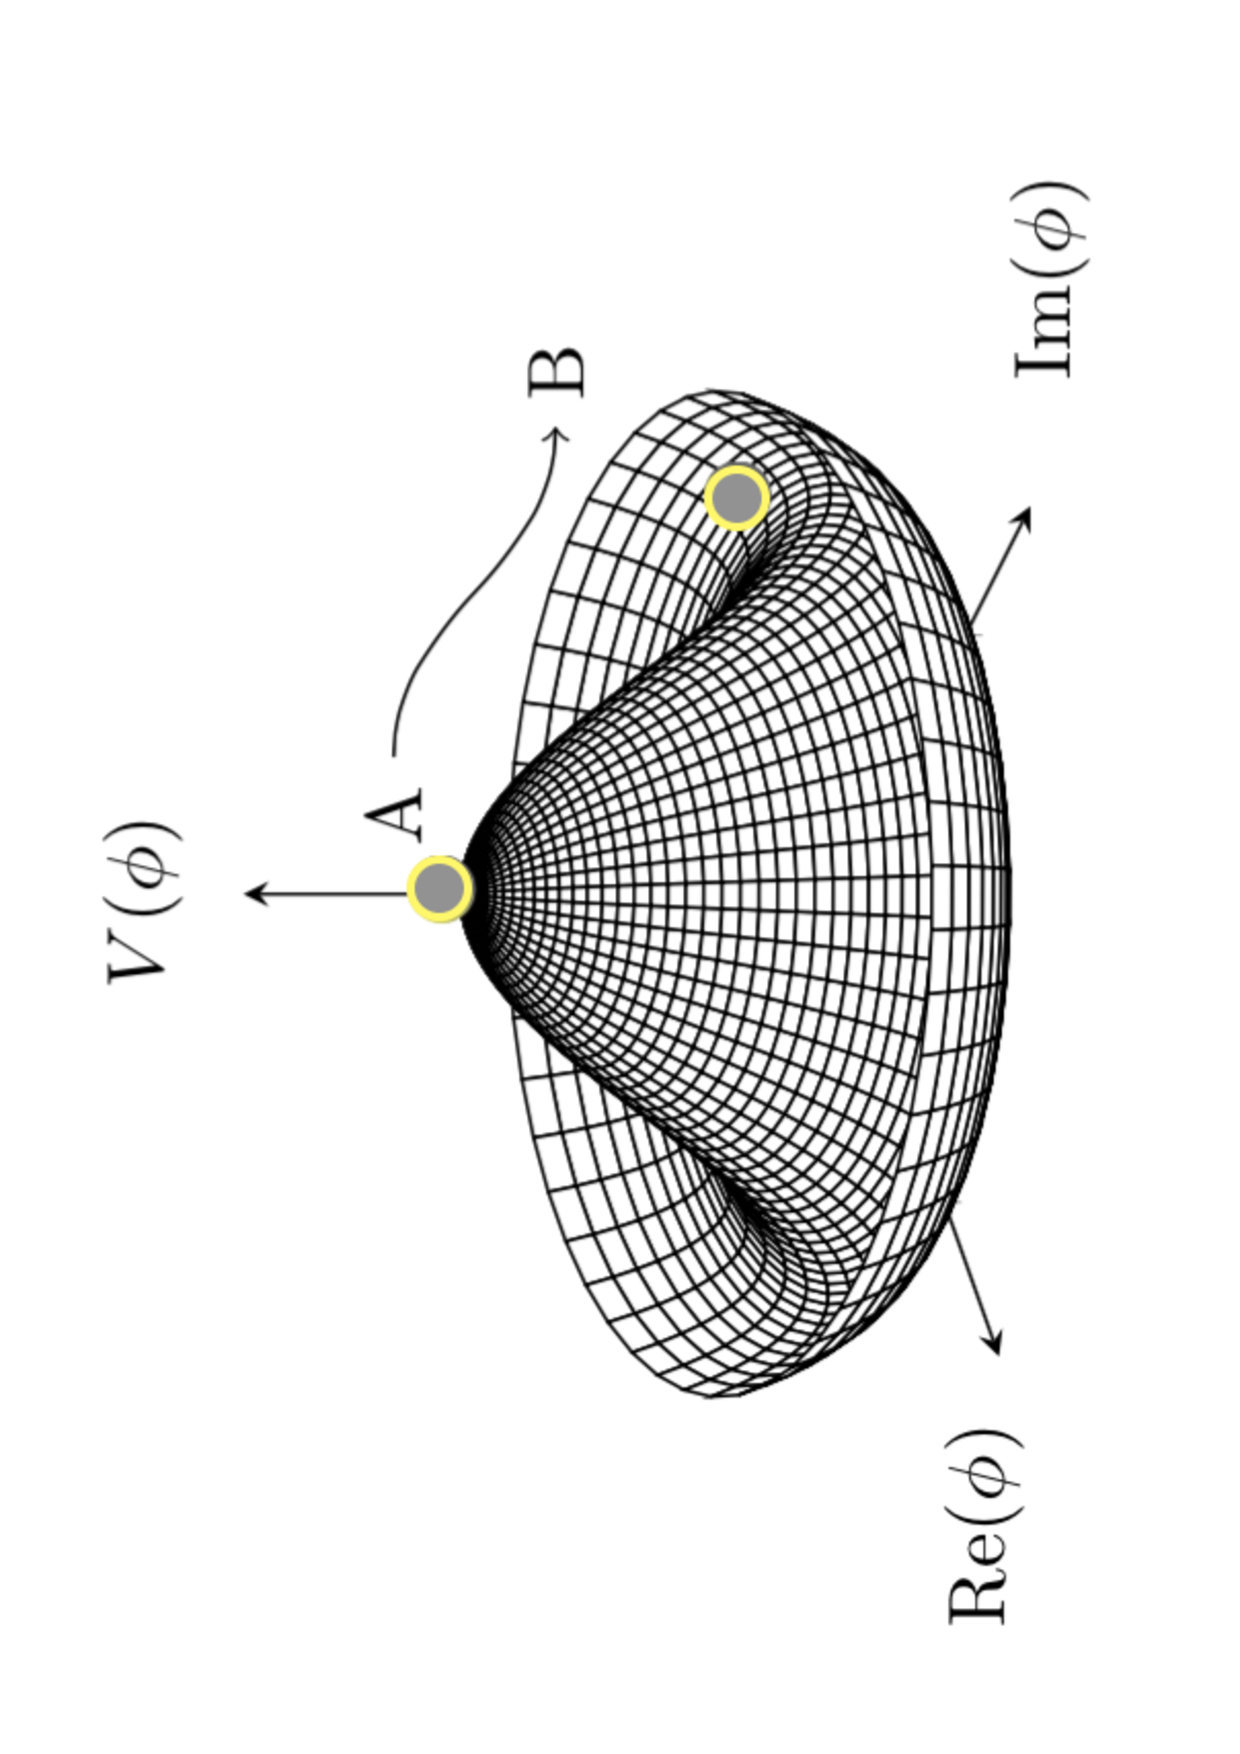
\includegraphics[angle=-90,width=0.7\textwidth]{images/mexican_hat.pdf}
  \caption{Illustration of the shape of the Higgs complex scalar potential with vacuum expectation value $v$. The symmetry is spontaneously broken when a singular ground state is chosen (A $\rightarrow$ B).}
  \label{res:mexican_hat}
\end{figure}

En este proceso, el campo de Higgs adquiere un valor esperado en el vacío distinto de cero (VEV, \(\langle H \rangle \approx 246\) GeV). Tres de los cuatro grados de libertad del doblete de Higgs se convierten en las componentes longitudinales de los bosones \(W^\pm\) y \(Z\), otorgándoles masa. El grado de libertad restante corresponde al bosón de Higgs físico, cuya masa fue medida en torno a \(125\) GeV.  

Además de explicar el origen de la masa de los bosones gauge, el mecanismo de Higgs también proporciona un marco para generar las masas de los fermiones. Este proceso se implementa mediante los acoplamientos de Yukawa, que conectan el campo de Higgs con los fermiones de manera proporcional a su masa. La fuerza de estos acoplamientos varía desde valores muy pequeños para electrones y neutrinos hasta valores del orden de la unidad para el quark top, el fermión más pesado conocido.  

El acoplamiento de Yukawa del quark top, \(y_{t}\), es de particular interés. Su magnitud determina directamente la probabilidad de procesos de producción como el \(\ttH\), en el que un Higgs se produce en asociación con un par top-antitop, constituyendo una medida directa de \(|y_{t}|\). Asimismo, la producción asociada con un solo quark top (\(tH\)) presenta una dependencia lineal con el acoplamiento de Yukawa del top, a diferencia de \ttH, cuya sección eficaz escala de manera cuadrática. Esta característica convierte al proceso en un observatorio privilegiado para explorar posibles fases intermedias de CP en la interacción, ya que la medida conjunta de \ttH\ y \(tH\) aporta información complementaria sobre la estructura del acoplamiento del Higgs al top~\cite{Bernreuther:2002uj,Brod:2013cka}. 

Las medidas experimentales de secciones eficaces de producción del bosón de Higgs se pueden interpretar dentro del marco de las \textit{Simplified Template Cross Sections} (STXS)~\cite{badger2016leshouches2015physics,STXS11}. Esta estrategia consiste en dividir el espacio de fase en regiones cinemáticas bien definidas, optimizadas para maximizar la sensibilidad experimental y minimizar dependencias teóricas.  

El esquema STXS permite combinar de manera coherente resultados de diferentes modos de desintegración y de producción, y se ha convertido en el estándar de la Colaboración ATLAS para caracterizar la física del Higgs. En el caso de procesos asociados al quark top, como \(\ttH\) y \(tH\), las categorías STXS diferenciadas en bins de momento transversal del Higgs \(p_{\text{T}}^{H}\) son especialmente relevantes para estudiar los acoplamientos de Yukawa y mejorar la sensibilidad en escenarios de nueva física.  

\begin{figure}[htbp]
  \centering
  \subfloat[]{
      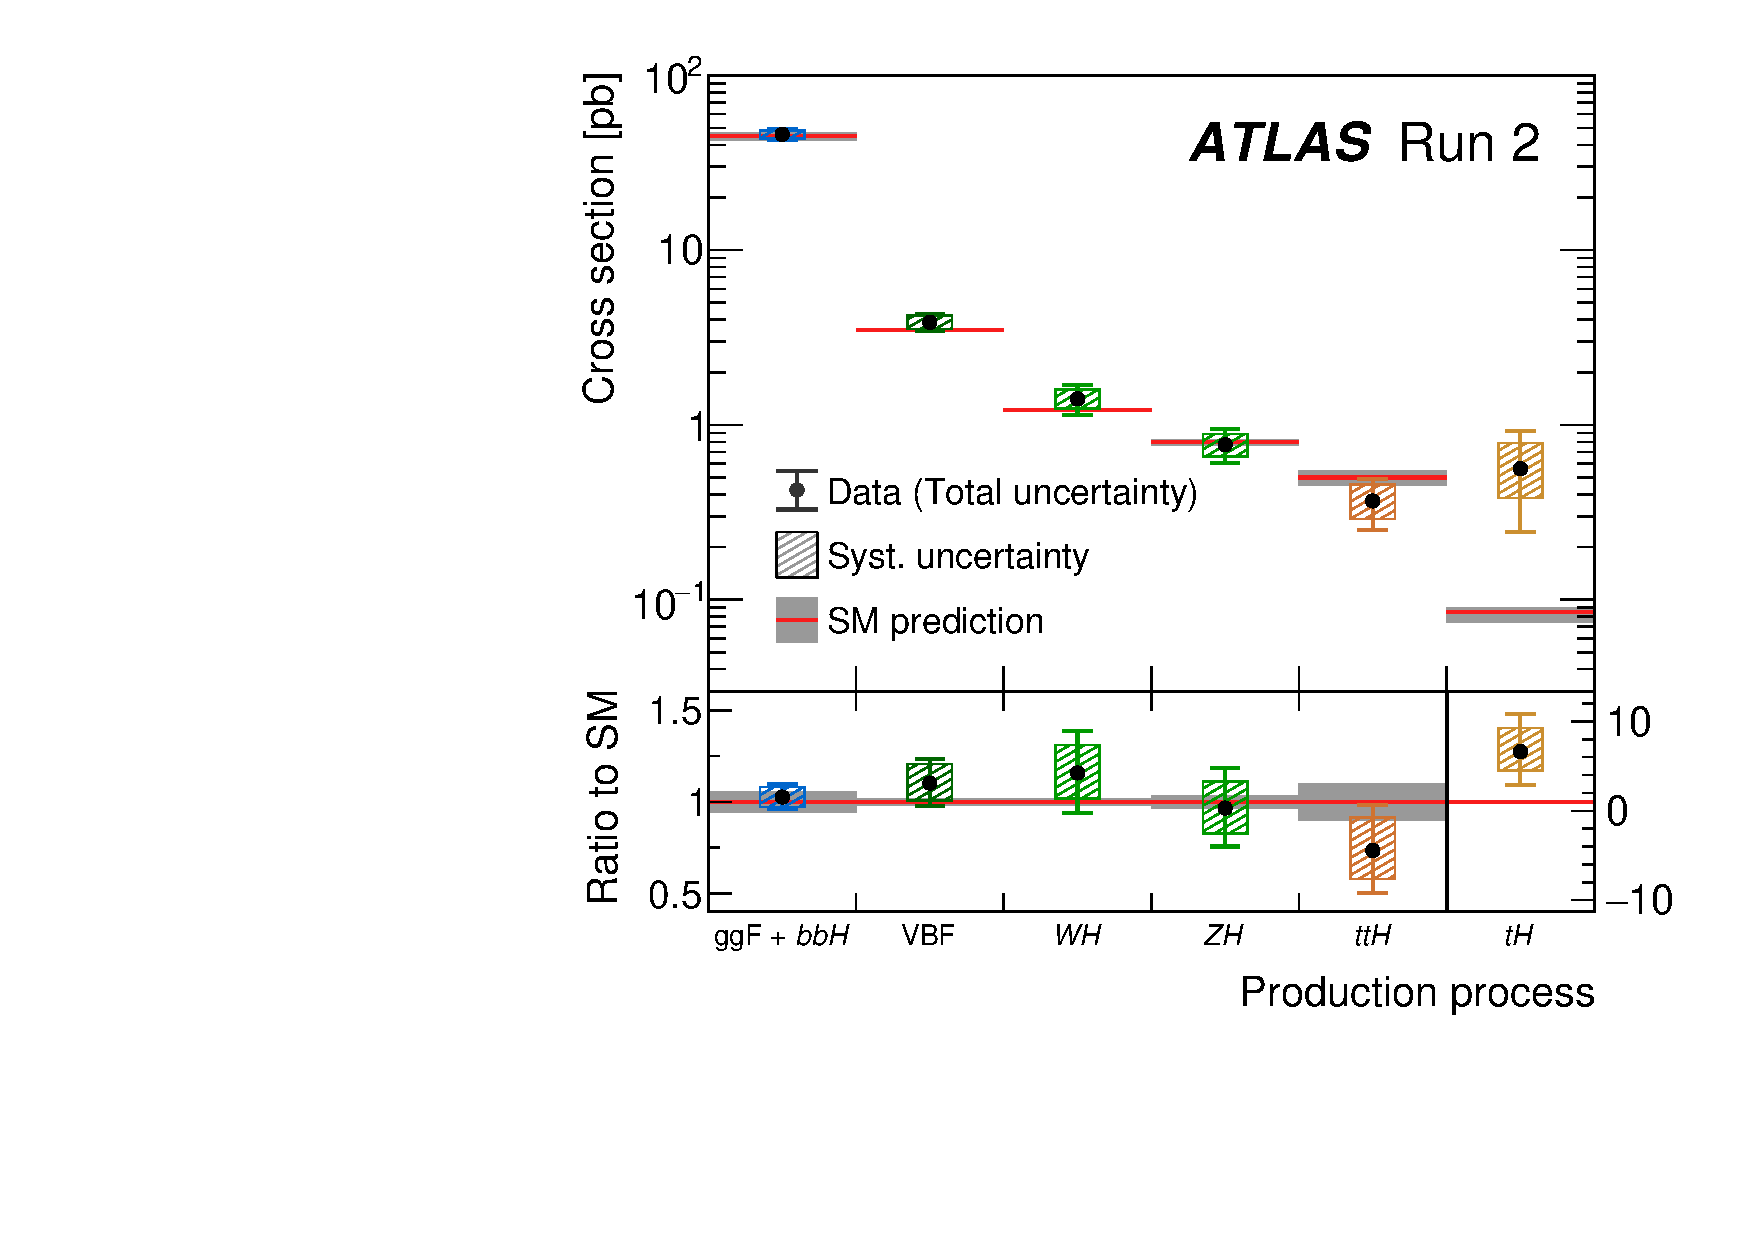
\includegraphics[width=0.46\textwidth]{atlas_combined_xsect.pdf}
  }
  \hfill
  \subfloat[]{
      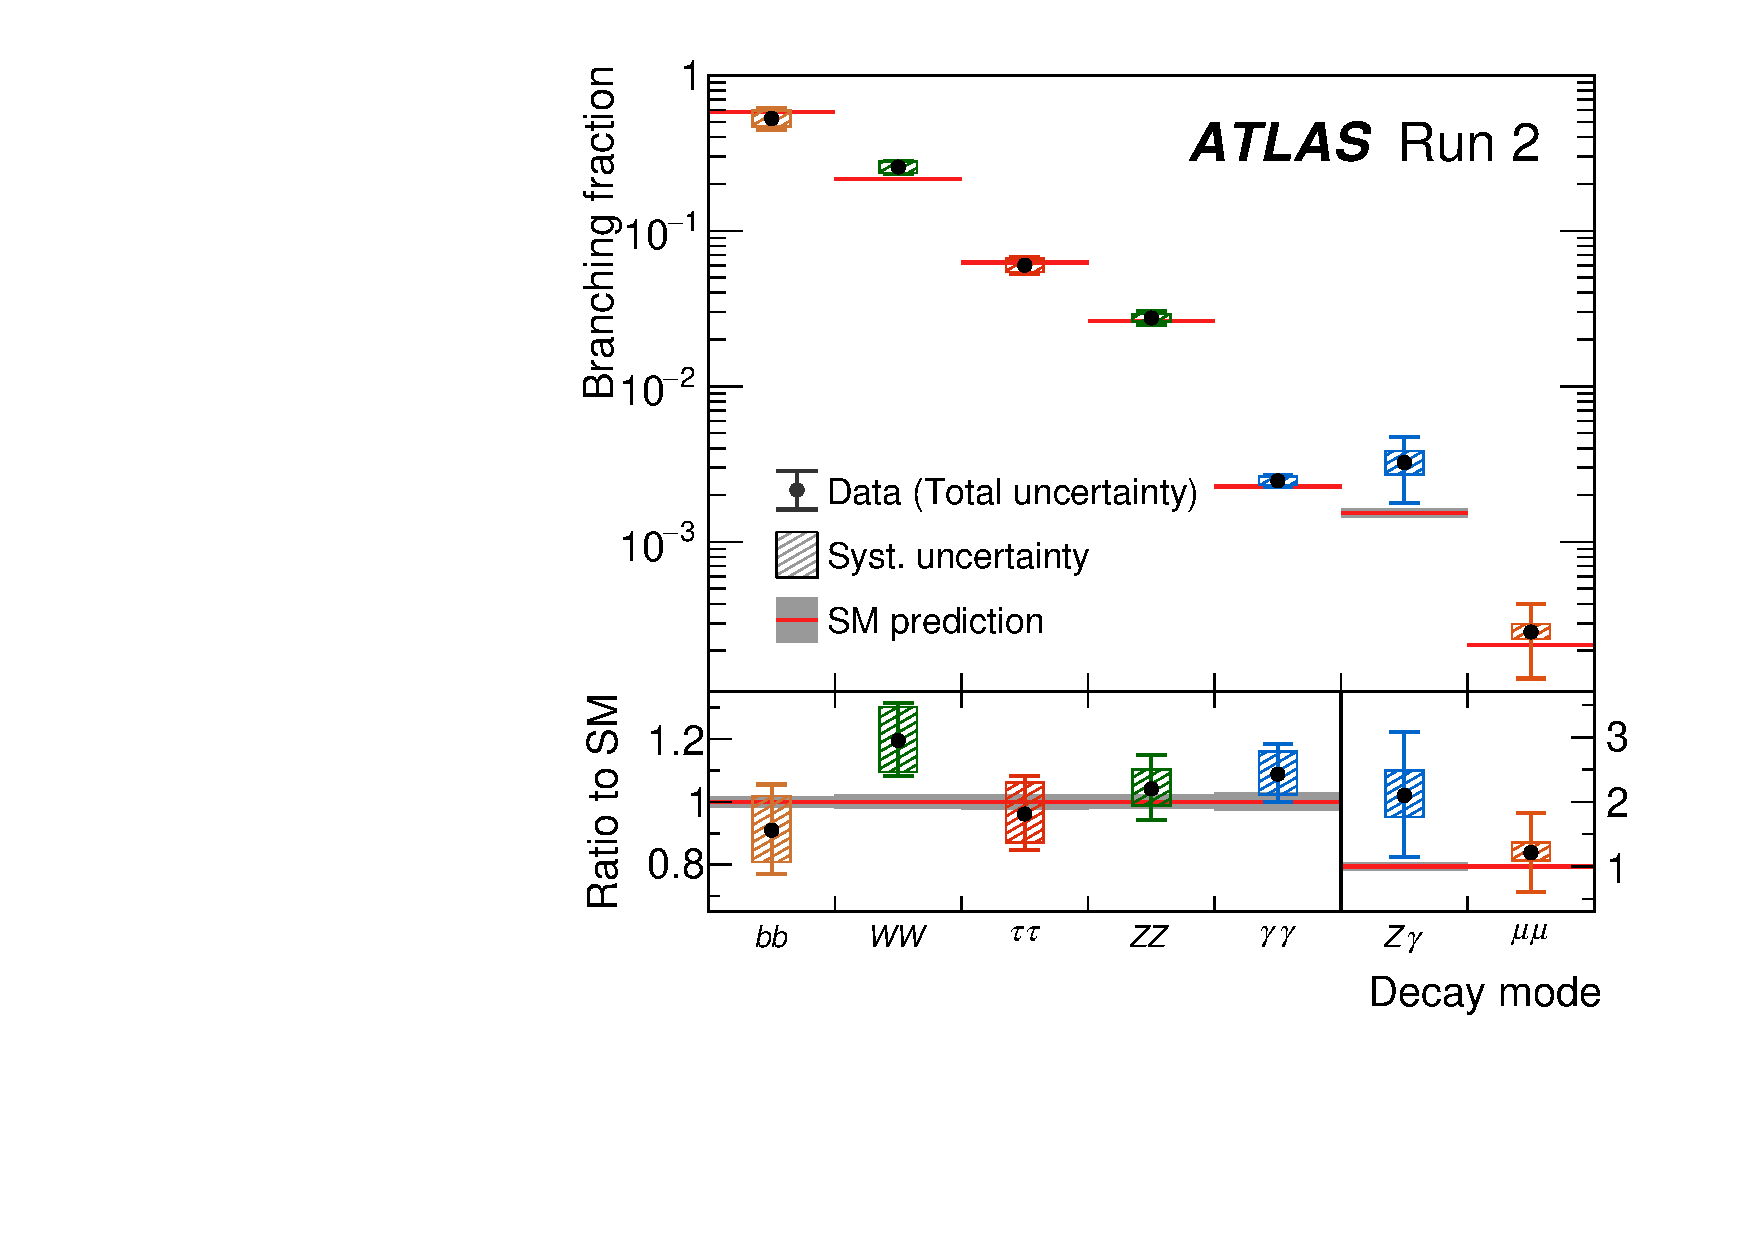
\includegraphics[width=0.46\textwidth]{atlas_combined_br.pdf}
  }
  \caption{(a) Summary of the Higgs boson production cross-sections assuming SM values for the Higgs boson branching ratios. 
  (b) Measurements of the Higgs boson decay branching ratios assuming SM predictions for the production cross-sections. 
  All results are obtained using ATLAS Run-2 data, combining different analyses, and are consistent with the SM predictions within uncertainties~\cite{Nature_ATLAS}.}
  \label{res:higgs_mu}
\end{figure}

El estudio detallado del bosón de Higgs constituye una de las principales prioridades del programa de física del LHC. La caracterización de sus acoplamientos a fermiones y bosones vectoriales no sólo sirve como prueba interna del Modelo Estándar, sino que también abre la puerta a explorar posibles desviaciones asociadas a teorías más allá del mismo, como supersimetría o modelos de Higgs compuestos.  

En este contexto, los análisis que explotan desintegraciones a leptones $\tau$ y la producción asociada con quarks top adquieren un papel central, al combinar sensibilidad a los acoplamientos fermiónicos de tercera generación con entornos experimentales complejos. 

%%%%%%%%%%%%%%%%%%%%%%%%%%%%%%%%%%%%%%%%%%%%%%%%%%%%%%%%%%%%%%%%%%%%%%%%%%%%%%%%%%%%%%%%%%%%%%%%%%%%%%%%%

\section*{El LHC y el detector ATLAS}

El Gran Colisionador de Hadrones (LHC, por sus siglas en inglés)~\cite{Evans:1129806, Bruning:782076} es el acelerador de partículas más potente construido hasta la fecha. Está situado en un túnel circular de 27 km de circunferencia a unos 100 metros de profundidad en la frontera franco-suiza, reutilizando la infraestructura previa del \textit{Large Electron–Positron Collider} (LEP). Fue diseñado para colisionar protones y iones pesados a energías sin precedentes, con el objetivo de explorar el sector del bosón de Higgs, la física de precisión del Modelo Estándar y la posible existencia de nueva física.

Los haces de protones son inyectados en el LHC a través de un complejo de pre-aceleradores que incluye el \textit{Linac}, el \textit{Proton Synchrotron} (PS) y el \textit{Super Proton Synchrotron} (SPS). Una vez en el anillo principal, los haces se mantienen mediante 1232 dipolos superconductores de 8.3 T que guían su trayectoria y cerca de 400 cuadrupolos que enfocan el haz. El sistema opera a temperaturas criogénicas de 1.9 K utilizando helio superfluido. 

Durante Run-2 (2015–2018) el LHC alcanzó colisiones protón-protón a $\sqrt{s} = 13$ TeV, con luminosidades integradas de aproximadamente $140~\text{fb}^{-1}$ para ATLAS y CMS. En Run-3 (2022–2025) la energía de colisión ha aumentado a 13.6 TeV, con el objetivo de acumular más de $300~\text{fb}^{-1}$. El futuro proyecto HL-LHC prevé incrementar este valor en un factor diez, alcanzando $3000~\text{fb}^{-1}$ de datos registrados por experimento, lo que permitirá explorar procesos raros con sensibilidad sin precedentes.

ATLAS~\cite{ATLAS:exp,ATLAS_run3} es uno de los dos detectores generales de propósito múltiple en el LHC. Con 44~m de longitud, 25~m de altura y un peso total de 7000 toneladas, es el detector de mayor volumen construido en un acelerador. Su diseño en capas concéntricas permite una cobertura casi completa en ángulo sólido, siendo capaz de registrar leptones, fotones, jets hadrónicos y energía perdida transversal en un amplio rango de energías.

\begin{center}
  \includegraphics[width=0.75\textwidth]{images/ATLAS-Experiment-Schematic-2022-Labels-People.png}
  \captionof{figure}{Vista esquemática del detector ATLAS, mostrando sus principales subsistemas: detector interno, calorímetros y espectrómetro de muones~\cite{Bianchi:2837191}.}
  \end{center}

\textbf{Detector interno (ID)~\cite{2010_id,ATLAS:exp}:} reconstruye trayectorias de partículas cargadas en el campo magnético de 2 T generado por un solenoide superconductor. Incluye el detector de píxeles, el SCT de tiras de silicio y el TRT. Es esencial para medidas de impacto, reconstrucción de vértices y separación entre electrones y hadrones.  

\textbf{Calorímetros~\cite{2010_lar,2010_tile}:} el calorímetro electromagnético, basado en argón líquido y plomo, ofrece gran resolución en energía para electrones y fotones. Los calorímetros hadrónicos, de azulejos centelleadores y argón líquido con cobre/tungsteno, permiten la medida de jets y energía perdida transversal.  

\textbf{Espectrómetro de muones~\cite{muon_com}:} situado en el exterior del detector y
ubicado en un campo magnético toroidal de 4~T, detecta los muones que atraviesan los
sistemas de calorimetría. Está compuesto por cuatro subsistemas:
\textit{Monitored Drift Tubes} (MDT) y \textit{Cathode Strip Chambers} (CSC) para medir el momento,
y \textit{Resistive Plate Chambers} (RPC) y \textit{Thin Gap Chambers} (TGC) para generar señales de \textit{trigger}.
La combinación de estos subsistemas permite medir la curvatura de las trayectorias de los muones

\textbf{Detectores \textit{Forward}:} ATLAS dispone de varios detectores hacia la dirección de los haces (LUCID~\cite{Jenni:721908} , ALFA~\cite{Khalek_2016}, AFP~\cite{Adamczyk:2015cjy} y ZDC~\cite{Jenni:1009649}) que extienden la cobertura a regiones de muy alto pseudorrapidez. Estos sistemas permiten medir la luminosidad relativa y absoluta, estudiar procesos de dispersión elástica, detectar protones muy adelantados y registrar partículas neutras en colisiones pesadas.

\textbf{Trigger~\cite{trigger_run2}:} el sistema de selección de eventos en tiempo real, con un primer nivel hardware (L1) y un posterior nivel basado en software (HLT), reduce la tasa de eventos de 40 MHz a aproximadamente 1 kHz, que se almacenan para su análisis.

El análisis de los datos registrados por ATLAS requiere una infraestructura computacional de gran escala. El experimento utiliza un sistema de computación distribuida basado en la \textit{Worldwide LHC Computing Grid} (WLCG)~\cite{Bird:1695401}, que conecta más de 170 centros en 40 países, proporcionando del orden de cientos de petabytes de capacidad de almacenamiento y potencia de cómputo equivalente a varios millones de núcleos de CPU.  

El flujo de datos sigue un esquema jerárquico en tres niveles: los \textit{Tier-0} en el CERN procesan en tiempo real la reconstrucción inicial; los \textit{Tier-1}, distribuidos internacionalmente, almacenan y recalibran los datos; y los \textit{Tier-2} y \textit{Tier-3} proporcionan recursos para simulaciones Monte Carlo (MC) y análisis por parte de los físicos.  

El software de ATLAS está basado en el framework \textsc{athena}~\cite{athena}, desarrollado en C++ y Python, que integra la simulación de eventos, la reconstrucción de objetos físicos y la aplicación de algoritmos de identificación. Las distintas versiones de \textsc{athena}, conocidas como \textit{releases}, definen la configuración oficial de reconstrucción y calibración utilizada en cada periodo de toma de datos. En paralelo, las campañas de producción MC (MC16 para Run-2, MC20 y MC23 para Run-3) proporcionan muestras coherentes con las condiciones de detector y de haz en cada época de operación del LHC.  

\section*{Datos y simulaciones}

Los análisis presentados en esta tesis se basan en datos de colisiones protón-protón registrados por ATLAS en Run-2 (2015–2018) y Run-3 (2022–2024), que suman $140~\text{fb}^{-1}$ a $\sqrt{s}=13$ TeV y unos $166~\text{fb}^{-1}$ a $\sqrt{s}=13.6$ TeV, respectivamente, tras aplicar los criterios de calidad de datos. Estos conjuntos se utilizan tanto para validar nuevas estrategias de identificación de electrones como para estudiar modos poco frecuentes de producción del bosón de Higgs, incluyendo \(\ttH\) y \(tHqb\).  

La modelización de las colisiones protón-protón en el LHC constituye un reto esencial, al involucrar múltiples escalas energéticas y procesos simultáneos~\cite{BUCKLEY2011145}. En QCD perturbativa, los protones se tratan como haces de partones (quarks y gluones) descritos por funciones de distribución de partones (PDFs), que definen la probabilidad de que un partón transporte una fracción $x$ del momento del protón. Los cálculos a órdenes NLO y NNLO proporcionan las secciones eficaces de los procesos duros, combinados con algoritmos de \textit{parton showering} que simulan la cascada de radiación partónica, seguidos de la hadronización en estados ligados de color neutro mediante modelos fenomenológicos. Además, se incluyen fenómenos colectivos como colisiones múltiples de partones (MPI) y el \textit{pile-up}, es decir, interacciones simultáneas en un mismo cruce de haces que afectan a la reconstrucción de objetos físicos.  

La simulación de estos procesos se realiza mediante campañas de producción Monte Carlo (MC) específicas para cada época de datos. El flujo típico consiste en la generación de eventos a nivel partónico con programas como \textsc{powheg}~\cite{Frixione_2007}, \textsc{madgraph5\_amc@nlo}~\cite{Alwall_2014} o \textsc{sherpa}~\cite{Bothmann_2019}, interfaseados con hadronizadores como \textsc{pythia8}~\cite{SJOSTRAND2015159} o \textsc{herwig}~\cite{B_hr_2008}, y posteriormente en la simulación detallada del detector con \textsc{geant4}~\cite{AGOSTINELLI2003250}.  

En los estudios de electrones se utilizan muestras dedicadas de $Z\to e^+e^-$ y $J/\psi \to e^+e^-$, fundamentales para validar la reconstrucción, estudiar la eficiencia de identificación y derivar factores de escala al comparar datos y MC. Los principales fondos que imitan electrones se modelan con procesos multijet QCD, desintegraciones de hadrones pesados ($b$, $c$) y fotones convertidos, utilizando muestras específicas como JF17 generadas con \textsc{pythia}~\cite{SJOSTRAND2015159}.  

En el caso del Higgs, los procesos de señal \(\ttH\) y \(tHqb\) se simulan a precisión NLO o NNLO, incluyendo la desintegración $H\to\tau\tau$. Los fondos dominantes (\(\ttbar\)+jets, $Z\to\tau\tau$+jets y multijets QCD) se normalizan a cálculos de orden superior cuando están disponibles (NNLO en el caso de Drell–Yan) y a medidas de luminosidad integrada. En todos los casos, los eventos MC se corrigen para reproducir las condiciones reales del detector, incluyendo calibraciones de energía y resoluciones de los distintos objetos físicos.  

\section*{Reconstrucción de objetos físicos}

Una vez que el HLT acepta un evento, los datos registrados en las colisiones se procesan de forma \textit{offline} con el fin de reconstruir las partículas emergentes de la interacción protón–protón. Las señales registradas en el ID, los calorímetros y el MS se combinan mediante algoritmos dedicados que permiten construir los diferentes objetos físicos, los cuales constituyen los ingredientes esenciales de todos los análisis realizados en ATLAS. Entre ellos se incluyen las trazas cargadas y los vértices de colisión, muones, electrones y fotones, jets (con algoritmos dedicados para clasificarlos según su sabor), leptones $\tau$ que decaen hadrónicamente, así como el momento transversal perdido ($E_{\mathrm{T}}^{\text{miss}}$).  

\begin{figure}[h]
  \centering
  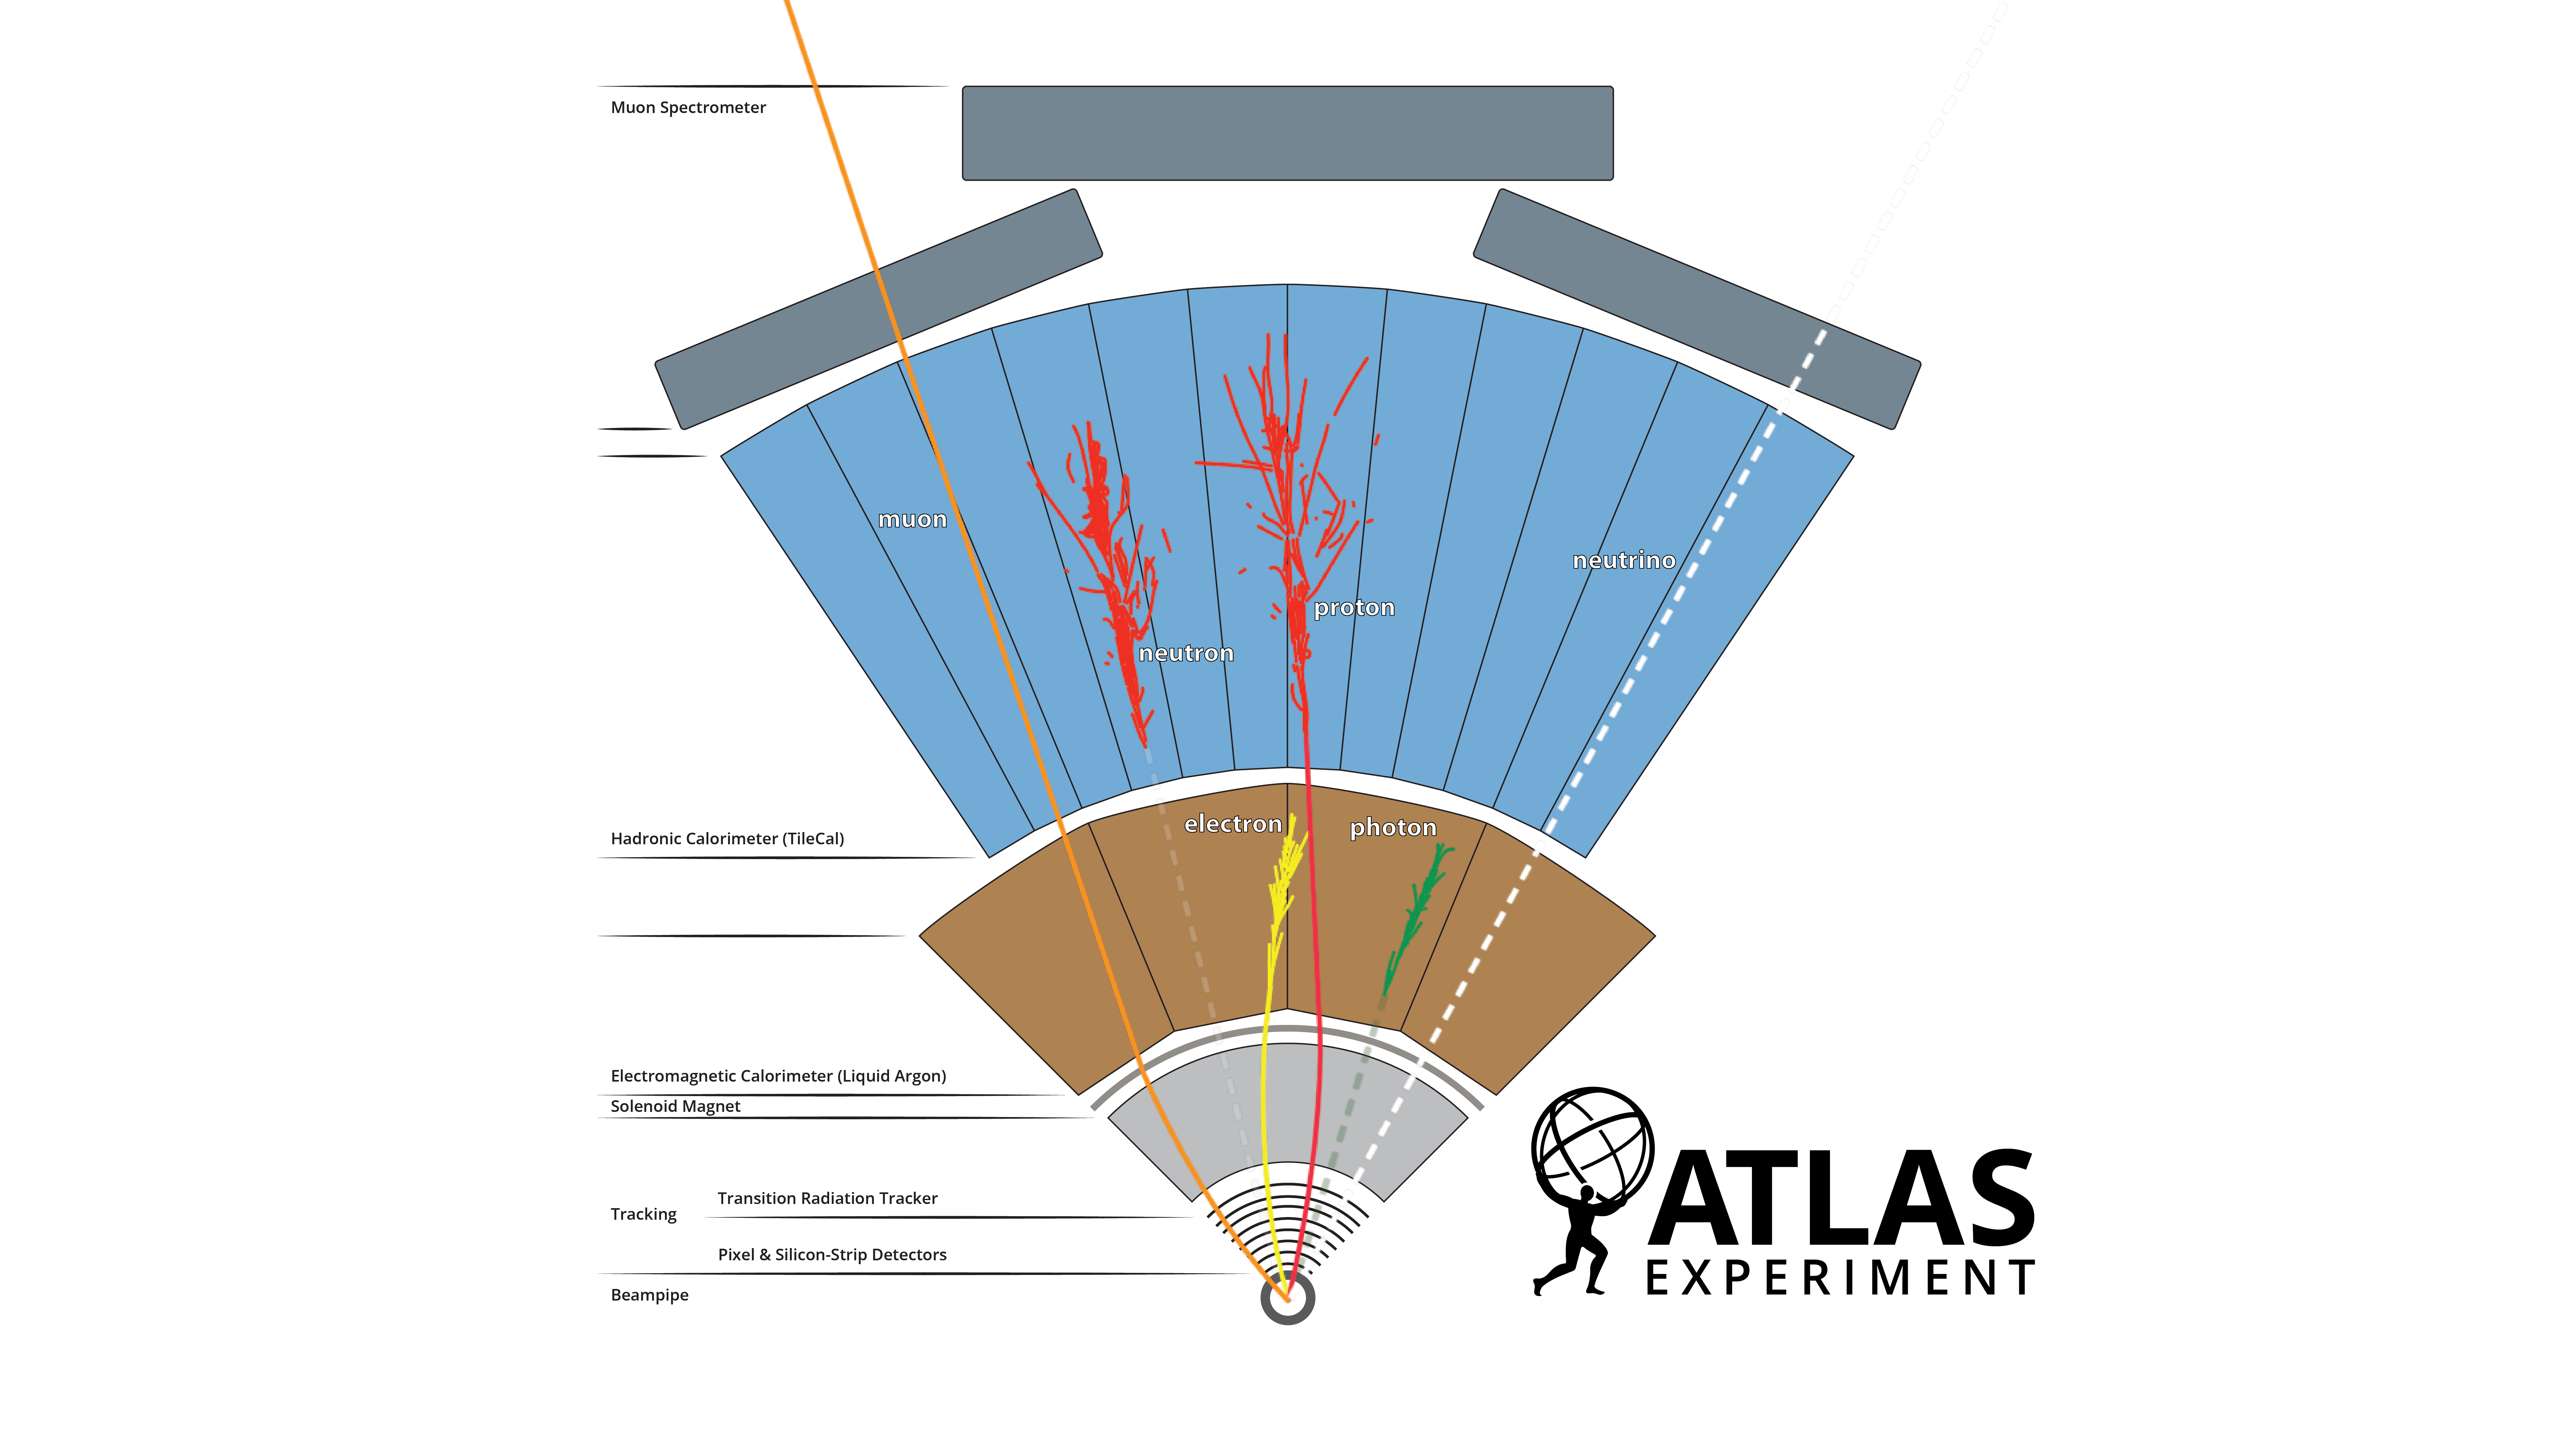
\includegraphics[width=0.9\textwidth]{images/atlas_particles.png}
  \caption{Esquema en el plano $x-y$ de particulas elementales interaccionando con los distintos subsistemas del detector ATLAS~\cite{Bianchi:2837191}.}
  \label{res:reco}
 \end{figure}

El primer paso en la reconstrucción es identificar las trayectorias de las partículas cargadas que atraviesan el detector interno~\cite{tracks}. Estas producen impactos precisos en los subdetectores de silicio (Pixel, SCT) y en el TRT, que bajo el campo magnético solenoidal de 2~T se curvan describiendo idealmente hélices. Cada traza reconstruida queda definida por cinco parámetros: el momento transversal ($p_{\mathrm{T}}$), los ángulos polares ($\theta, \phi$), y los parámetros de impacto transversal y longitudinal ($d_{0}, z_{0}$).  

A partir de las trazas, se reconstruyen los vértices de interacción~\cite{vertex_run1,vertex_run2,vertex_run3}. El vértice primario corresponde al punto de la colisión dura, identificado como aquel con la mayor suma de $p_{\mathrm{T}}^{2}$ de las trazas asociadas, mientras que otros vértices se clasifican como \textit{pile-up} o secundarios. Estos últimos son esenciales para el etiquetado de sabor y la identificación de partículas desplazadas.

Tras pasar por el detector interno, las partículas depositan su energía en las celdas de los calorímetros, que se agrupan en clústeres tridimensionales denominados \textit{topoclusters}. El algoritmo comienza a partir de celdas semilla con señal significativa respecto al ruido electrónico y expande iterativamente a celdas adyacentes. Posteriormente, se aplican calibraciones específicas que corrigen las pérdidas en materiales pasivos y la diferente respuesta hadrónica y electromagnética. Durante Run-2 se introdujo además el concepto de \textit{superclúster}, que agrupa dinámicamente varios topoclusters, mejorando la recuperación de energía perdida por radiación de bremsstrahlung.

Los muones se reconstruyen combinando información del ID y del MS~\cite{muon_reco_run2}, dado su carácter de partículas mínimamente ionizantes que atraviesan el detector con escasa pérdida de energía. Existen distintas categorías de reconstrucción: muones combinados (ajuste conjunto ID+MS), extrapolados (MS únicamente), segment-tagged (traza del ID asociada a un segmento en el MS) y calorimeter-tagged (basados en depósitos mínimos de energía en el calorímetro alineados con una traza del ID). La identificación define distintos \textit{working points} (WPs, Loose, Medium, Tight, entre otros) que equilibran eficiencia frente a rechazo de fondo.

Los jets se reconstruyen a partir de los clústeres de energía usando algoritmos de recombinación como \texttt{anti-$k_{t}$}~\cite{Cacciari_2008}. Posteriormente se aplican correcciones de energía y calibraciones \textit{in-situ} para reproducir la respuesta del detector~\cite{jets_calib}. Un aspecto fundamental es el etiquetado de jets de sabor pesado, en particular de $b$-jets provenientes de desintegraciones de quarks top o del bosón de Higgs. Este etiquetado se realiza con algoritmos multivariantes como DL1r~\cite{tagging}, que explotan información de vértices secundarios y trazas desplazadas.

Los taus que decaen hadrónicamente se reconstruyen a partir de jets calibrados, identificando candidatos visibles ($\tau_{\text{had-vis}}$) con una o tres trazas asociadas. Algoritmos específicos, como redes recurrentes (RNN)~\cite{ATL-PHYS-PUB-2022-044}, permiten separar estos objetos de jets hadrónicos ordinarios, mientras que discriminantes adicionales como eBDT reducen la contaminación de electrones. Se definen WPs con eficiencias en torno al 75\% (1-prong) y 60\% (3-prong), utilizados en los análisis de Higgs a $\tau\tau$.

El $E_{\mathrm{T}}^{\text{miss}}$ se calcula como la suma vectorial negativa de los momentos transversales de todos los objetos reconstruidos en el evento, complementados con contribuciones de energía no asociadas a objetos. Es una magnitud esencial para identificar partículas neutras no detectadas, como neutrinos, y juega un papel clave en análisis de física electrodébil y de Higgs.  

En conjunto, la reconstrucción de objetos físicos proporciona la base sobre la que se construyen las estrategias de análisis. Su precisión e identificación eficiente son determinantes para alcanzar sensibilidad en procesos de baja sección eficaz como \ttH o \thqb, y garantizan la robustez de las medidas presentadas en esta tesis.

\section*{Reconstrucción, identificación y medidas de eficiencia de electrones}

Los electrones desempeñan un papel fundamental en el programa de física de ATLAS, al aparecer en estados finales clave desde medidas de precisión electrodébil hasta estudios del bosón de Higgs y búsquedas de nueva física. Por este motivo, la reconstrucción precisa, la identificación eficiente y las medidas de eficiencia con correcciones de factores de escala resultan cruciales. En esta sección se resume el trabajo de esta tesis en este ámbito, destacando la transición de los métodos tradicionales basados en likelihood hacia un nuevo algoritmo de identificación fundamentado en redes neuronales profundas (DNN). 

La reconstrucción de electrones en ATLAS comienza con la identificación de \textit{topoclusters}~\cite{dyn_clust} en el calorímetro electromagnético. Estos clusters dinámicos, definidos a partir de semillas con alta significancia sobre el ruido, crecen incorporando celdas vecinas hasta formar agrupaciones de energías representativas de las shower electromagnéticas. A continuación, se realiza la asociación con trazas reconstruidas en el detector interno. Para modelar la pérdida de energía por bremsstrahlung, se emplea el algoritmo Gaussian Sum Filter~\cite{FRUHWIRTH1987444}, que permite describir trayectorias con cambios bruscos de curvatura debidos a emisiones de fotones. La combinación de clusters y trazas da lugar a los denominados \textit{superclusters}~\cite{Aad:2684552}, que incluyen la energía radiada y permiten una reconstrucción más completa del electrón. Finalmente, las medidas de energía se calibran mediante regresiones BDT entrenadas en simulación, corrigiendo diferencias residuales entre datos y MC.  

\begin{figure}[htbp]
  \centering
  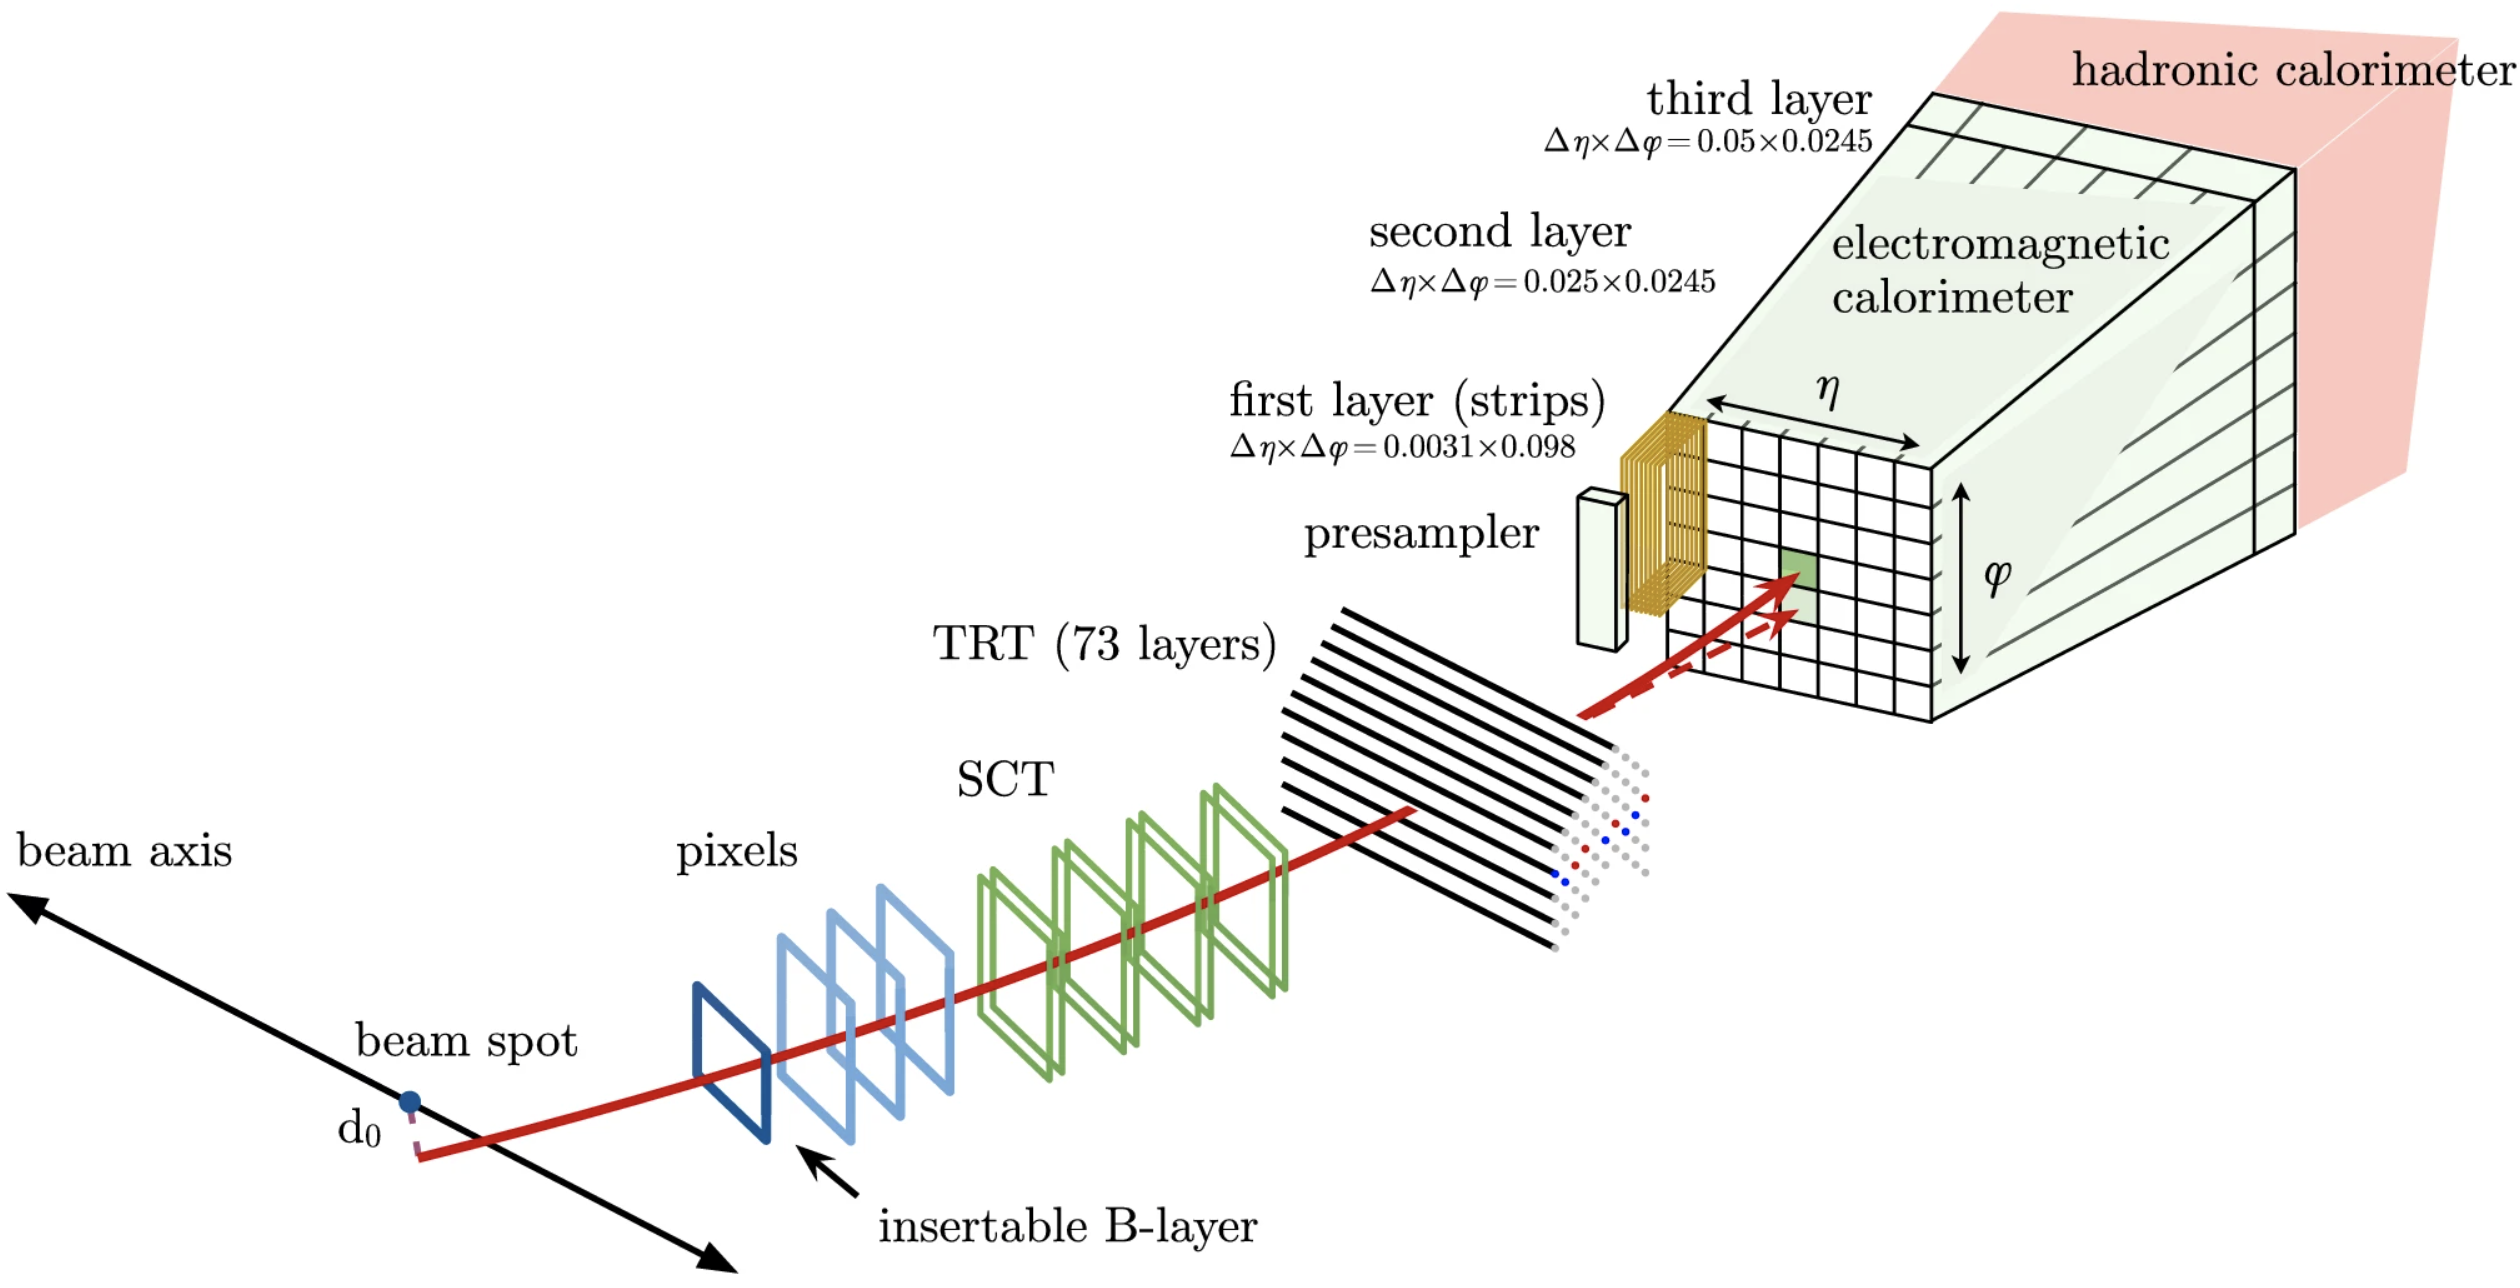
\includegraphics[width=0.9\textwidth]{images/electron_journey.png}
  \caption{Illustration of the typical journey of an electron passing through ATLAS. In red it is represented its expected path, first going through the tracking system. Afterwards it leaves mostly all its energy in the electromagnetic calorimeter. It can be also found the possible path (dashed red) of photon radiated by bremsstrahlung when the electron interacts with the material~\cite{Aaboud:2657964}.}
  \label{res:electron_journey}
\end{figure}

Tras la reconstrucción, es necesario aplicar algoritmos de identificación para separar electrones genuinos de otras partículas que imitan la señal que dejan en el detector, como piones cargados, conversiones de fotones o electrones no aislados de desintegraciones hadrónicas. Durante Run~2 se utilizó un discriminante basado en \textit{likelihood} (LH)~\cite{Aad:2684552,Aaboud:2657964}, construido a partir de PDFs unidimensionales de variables relacionadas con las características de las shower electromagnéticas, información de trazas y asociación calorímetro-traza. Este enfoque, aunque efectivo, pierde las correlaciones entre variables y presenta limitaciones en regiones complejas del detector.  

Para tratar de mejorar el rendimiento en identificación de electrones y rechazo de fondo, esta tesis introduce un nuevo discriminante basado en DNN, entrenado con múltiples clases de electrones: señal (electrones prompt y \textit{charge-flip}) y fondos (conversiones, heavy flavour, light flavour leptónicos y hadrónicos). El uso de seis clases permite capturar mejor la diversidad de orígenes de los candidatos electrónicos y optimizar la separación frente a los principales fondos.  

\begin{table}[h!]
  \centering
  \scriptsize
  \caption{Definición de las seis clases de candidatos a electrón utilizadas para entrenar la DNN y a lo largo de esta tesis. Adaptado de Ref.~\cite{dnn_paper}.}
  \begin{tabular}{@{}l p{6.2cm} c c@{}}
    \toprule
    \textbf{Clase} & \textbf{Descripción} & \textbf{Etiqueta} & \textbf{Muestra} \\
    \midrule
    Electrones \textit{Prompt} & Electrones primarios procedentes de desintegraciones primarias como $Z \rightarrow ee$, $W \rightarrow e\nu$ o $J/\psi \rightarrow ee$, incluyendo FSR o bremsstrahlung si el origen es un electrón prompt. La carga reconstruida debe coincidir con la de verdad. & \texttt{El} & \begin{tabular}[c]{@{}c@{}}$Z\rightarrow ee$ \\ $J/\psi \rightarrow ee$\end{tabular} \\
    \midrule
    \textit{Charge-flips} & Electrones primarios con carga mal reconstruida, principalmente debido a ambigüedades en las trazas. En caso de bremsstrahlung, se considera como carga de verdad la del electrón primario original. & \texttt{CF} & \begin{tabular}[c]{@{}c@{}}$Z\rightarrow ee$ \\ $J/\psi \rightarrow ee$\end{tabular} \\
    \midrule
    Conversiones de fotón & Electrones procedentes de conversiones de fotones puntuales en pares $e^{+}e^{-}$. También se incluyen fotones puntuales mal reconstruidos como electrones. & \texttt{PC} & $\text{JF}17$, \ttbar \\
    \midrule
    Electrones de \textit{Heavy Flavour} & Electrones de desintegraciones semileptónicas de hadrones pesados con quarks $b$ o $c$. Normalmente no aislados y con vértice ligeramente desplazado. & \texttt{HF} & $\text{JF}17$, \ttbar \\
    \midrule
    $e/\gamma$ de \textit{Light flavour} & Electrones o fotones procedentes de desintegraciones de hadrones de quarks ligeros, incluyendo conversiones intermedias como $\pi^0 \rightarrow \gamma\gamma$ seguidas de $\gamma \rightarrow ee$. & \texttt{LFEg} & $\text{JF}17$ \\
    \midrule
    Hadrones de \textit{Light Flavour} & Hadrones mal identificados como electrones debido a depósitos de energía anómalos en el calorímetro electromagnético. & \texttt{LFH} & $\text{JF}17$ \\
    \bottomrule
  \end{tabular}
  \label{res:electron_classes}
\end{table}

Las variables de entrada incluyen tanto observables calorimétricos (anchura de las showers, fugas en el calorímetro hadrónico, fracciones de energía por capa) como de trazas (impacto transversal $d_0$, número de hits en Pixel y SCT, probabilidad TRT) y asociación traza-calorímetro ($E/p$, $\Delta\eta$, $\Delta\phi$). En total, más de 20 variables fueron utilizadas, aplicando un preprocesado cuidadoso: aplicación de correcciones \textit{shift\&stretch} para mejorar el acuerdo datos-MC, y técnicas de \textit{downsampling} y \textit{reweighting} para armonizar las distribuciones de $E_T$ y $\eta$ entre clases de electrones antes de introducirlos como entradas en la red neuronal.
Posteriormente, todas las variables se transformaron mediante cuantiles a distribuciones uniformes, optimizando el entrenamiento.  
% === Figure B: rows 4–6 (6 panels) ===
\begin{figure}[htbp]
  \centering
  % Row 4
  \begin{subfigure}[b]{0.49\textwidth}
    \centering
    \includegraphics[width=\linewidth]{normalized_weighted_distributions/weighted_Multiclass_wtots1_train.pdf}
    \caption{$w_{stot}$}
    \label{fig:input7}
  \end{subfigure}\hfill
  \begin{subfigure}[b]{0.49\textwidth}
    \centering
    \includegraphics[width=\linewidth]{normalized_weighted_distributions/weighted_Multiclass_eratio_train.pdf}
    \caption{$E_{\text{ratio}}$}
    \label{fig:input8}
  \end{subfigure}
  \vspace{0.45cm}
  % Row 5
  \begin{subfigure}[b]{0.49\textwidth}
    \centering
    \includegraphics[width=\linewidth]{normalized_weighted_distributions/weighted_Multiclass_f1_train.pdf}
    \caption{$f_1$}
    \label{fig:input9}
  \end{subfigure}\hfill
  \begin{subfigure}[b]{0.49\textwidth}
    \centering
    \includegraphics[width=\linewidth]{normalized_weighted_distributions/weighted_Multiclass_npixel_train.pdf}
    \caption{$n_{\text{Pixel}}$}
    \label{fig:input11}
  \end{subfigure}
  \vspace{0.45cm}
  % Row 6
  \begin{subfigure}[b]{0.49\textwidth}
    \centering
    \includegraphics[width=\linewidth]{normalized_weighted_distributions/weighted_Multiclass_nsilicon_train.pdf}
    \caption{$n_{\text{Si}}$}
    \label{fig:input12}
  \end{subfigure}\hfill
  \begin{subfigure}[b]{0.49\textwidth}
    \centering
    \includegraphics[width=\linewidth]{normalized_weighted_distributions/weighted_Multiclass_TRTPID_train.pdf}
    \caption{TRT PID}
    \label{fig:input18}
  \end{subfigure}
  \caption{Distribuciones de algunas de las variables de entrada utilizadas para el entrenamiento de la DNN, tras los procedimientos de preprocesado.}
  \label{fig:dnn_inputs_distributions_B}
\end{figure}

La arquitectura de la DNN implementada consta de cinco capas ``ocultas'' de 256 nodos cada una, aplicando funciones Leaky ReLU para la activación y normalización por \textit{batch}. La salida es multinomial, con seis nodos y función Softmax, lo que permite obtener probabilidades para cada clase. 
A partir de estas salidas se construye un discriminante binomial $D_{el}$ que combina señal frente a fondos, con pesos $f_X$ optimizados maximizando el área bajo la curva ROC. También se definió un discriminante $D_{CF}$ enfocado a separar electrones de señal con carga correctamente reconstruida de \textit{Charge Flips}, ofreciendo también un gran poder separatorio.  

\begin{figure}[htbp]
  \centering
  \begin{subfigure}[t]{0.48\linewidth}
    \centering
    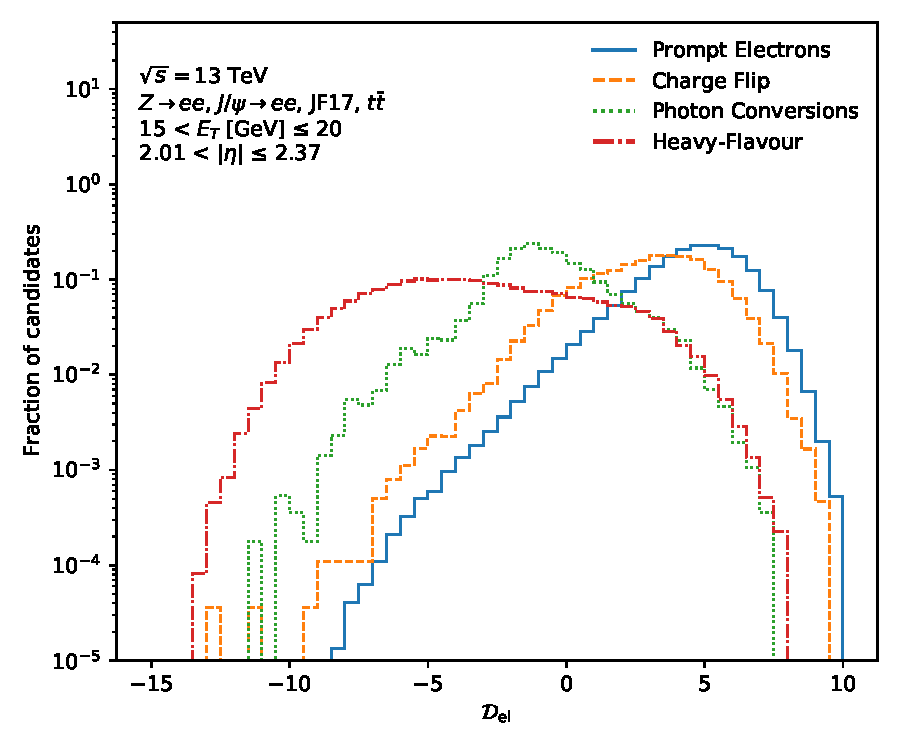
\includegraphics[width=\linewidth]{discriminant_plots/panel_a.pdf}
    \caption{}
    \label{fig:dnnDisc_a}
  \end{subfigure}\hfill
  \begin{subfigure}[t]{0.48\linewidth}
    \centering
    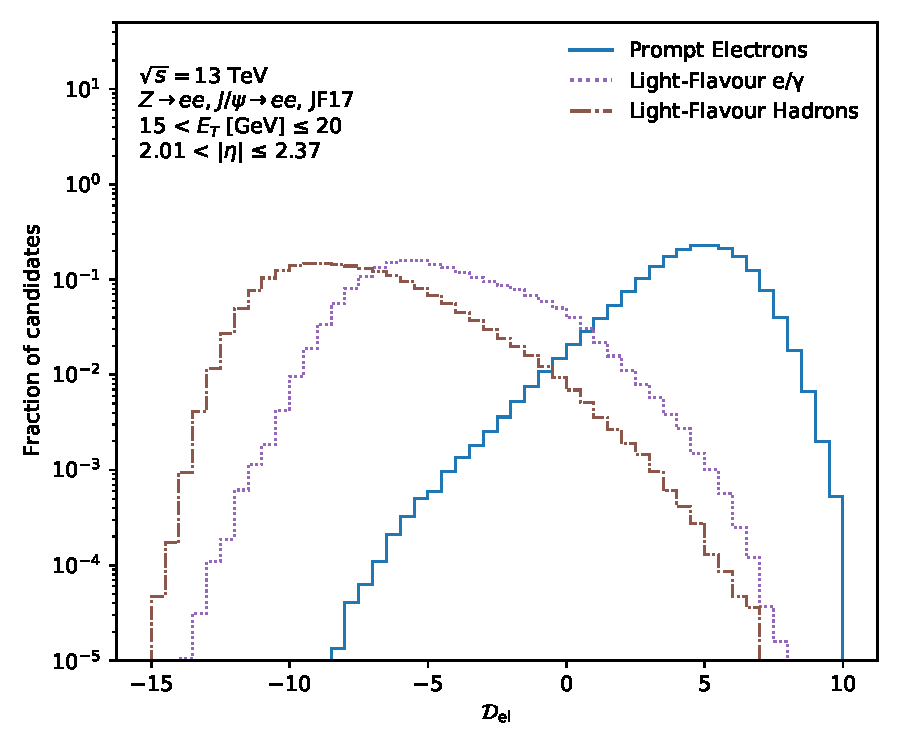
\includegraphics[width=\linewidth]{discriminant_plots/panel_b.pdf}
    \caption{}
    \label{fig:dnnDisc_b}
  \end{subfigure}

  \caption{$D_{\mathrm{el}}$ de la DNN mostrado para (a) electrones primarios, CF y fondos de PC y HF; y (b) electrones primarios y fondos de LFEg y LFH. Los candidatos a electrón cumplen $15<E_{T}\leq 20~\mathrm{GeV}$ y $0.0<|\eta|\leq 0.8$}
  \label{res:dnn_final_disc_ab}
\end{figure}

Los resultados obtenidos reflejan que se espera una mejora clara respecto al LH. En el WP Loose, el rechazo de fondos combinado mejora por un factor $\sim2$. Para HF el rechazo es $\sim2.2$ veces superior, mientras que para LFEg y LFH la mejora alcanza factores 4–5. En PC el incremento es de un factor $\sim2$, y en CF, gracias a nuevas variables ($q\times d_0$, $q_{\text{SCT}}$), la mejora es casi de un factor 8.  

\begin{figure}[h]
  \centering
  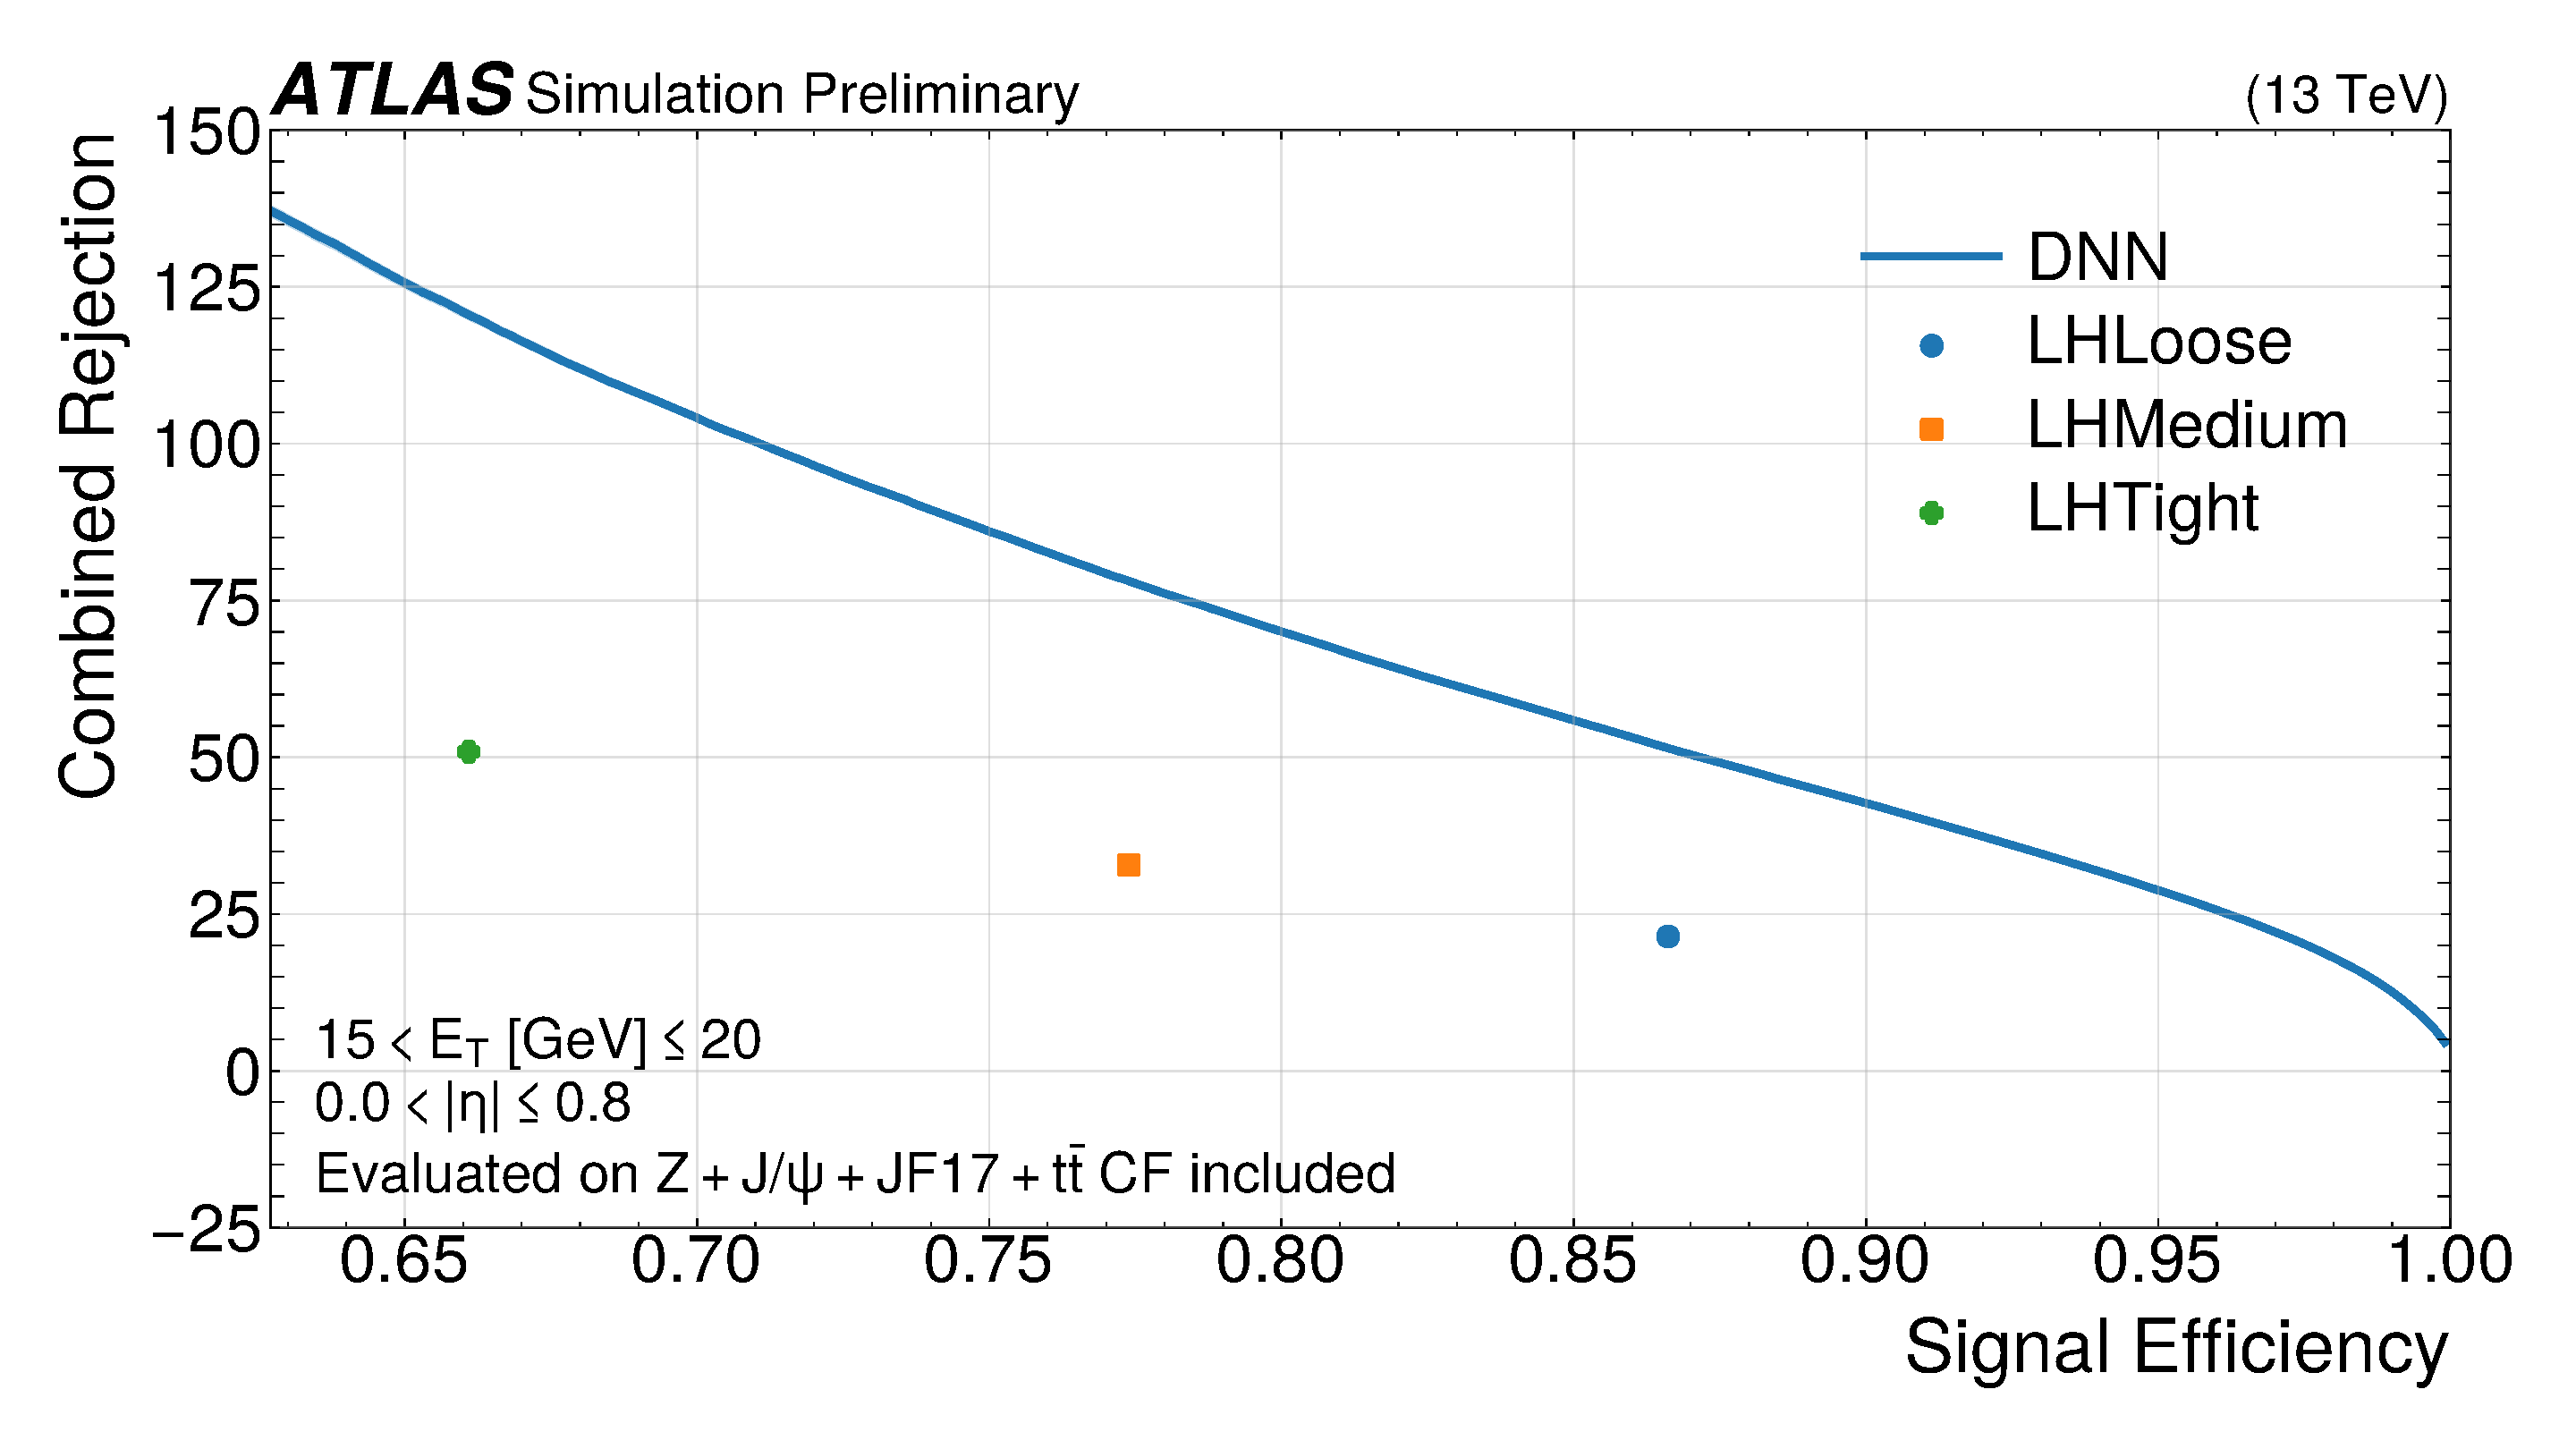
\includegraphics[width=0.7\linewidth]{ROC/15_20_0p0_0p8/binnedROCCurve_et15_20_eta0.0_0.8.pdf}
  \caption{Rechazo de fondo frente a eficiencia de señal (curvas ROC) para electrones primarios frente a todas las clases de fondo combinadas en un bin representativo de $(E_{T}, |\eta|)$. La incertidumbre estadística del rechazo de fondo se muestra como una banda.}
  \label{fig:roc_allblkg}
\end{figure}


% --- Primera figura ---
\begin{figure}[h]
  \centering
  % ---- Fila 1 ----
  \begin{subfigure}[t]{0.5\linewidth}
    \centering
    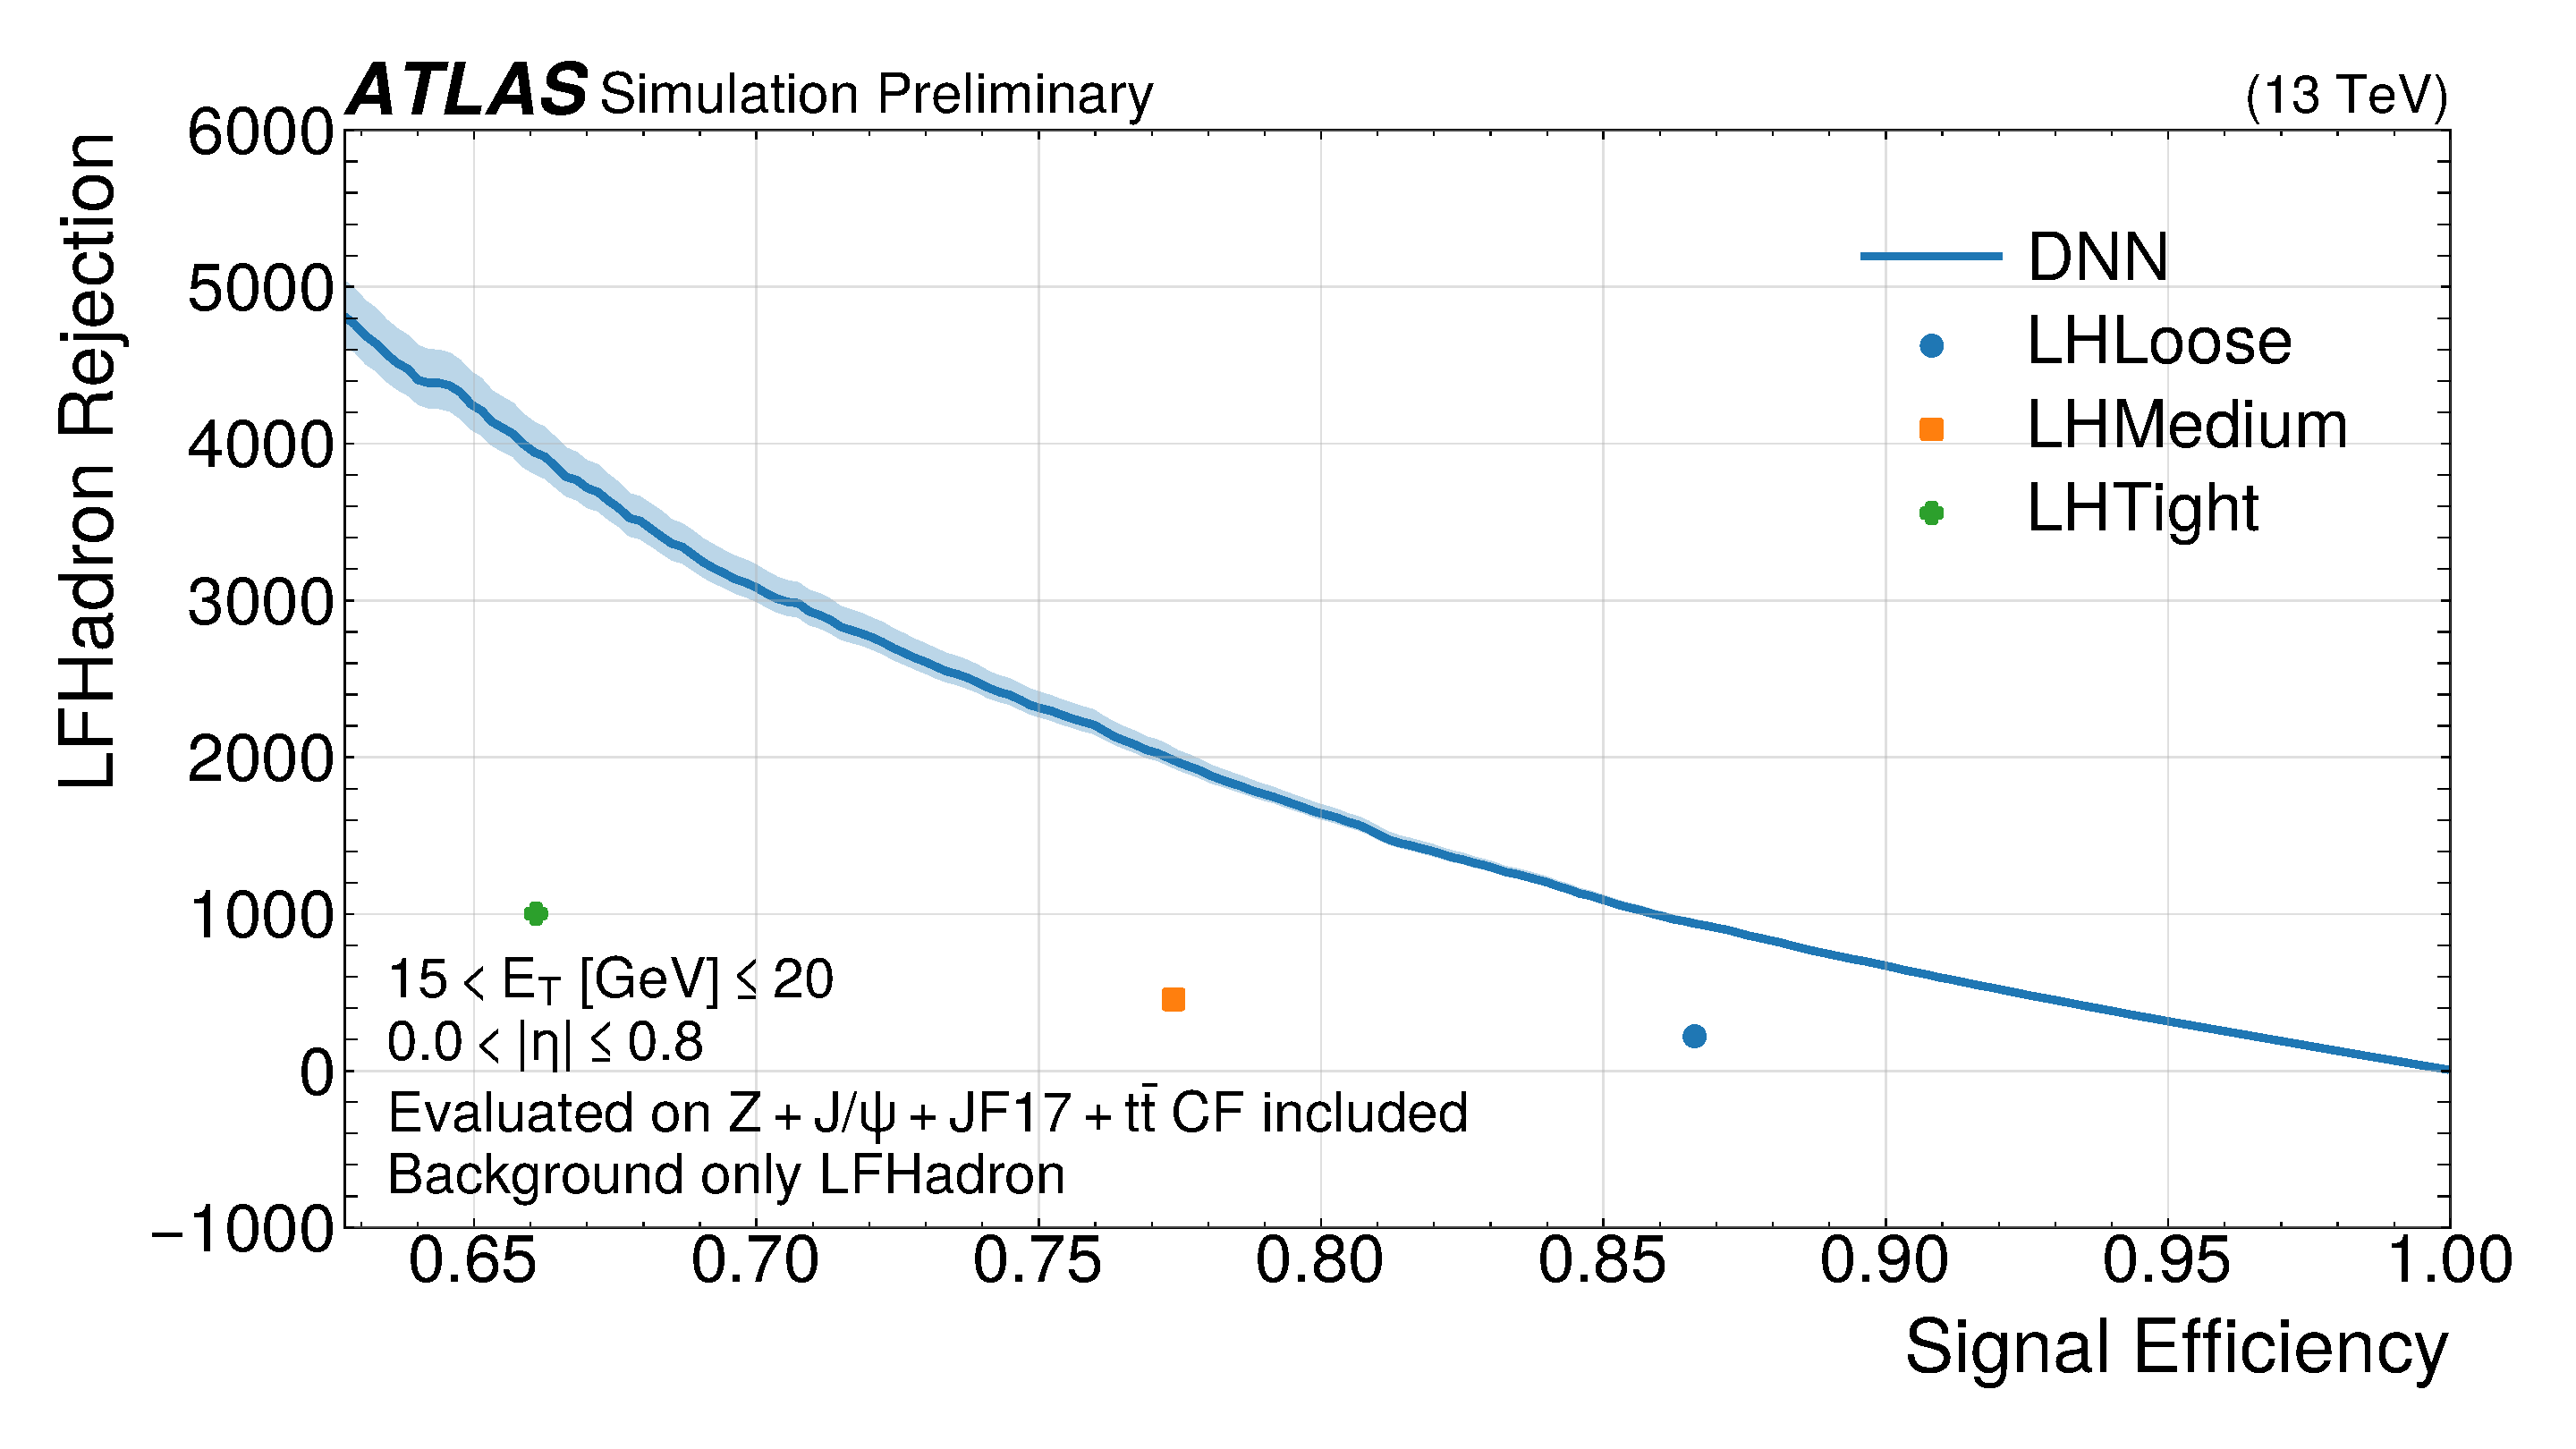
\includegraphics[width=\linewidth]{ROC/15_20_0p0_0p8/binnedROCCurveLFHadron_et15_20_eta0.0_0.8.pdf}
    \caption{}
    \label{fig:roc_pc}
  \end{subfigure}\hfill
  \begin{subfigure}[t]{0.5\linewidth}
    \centering
    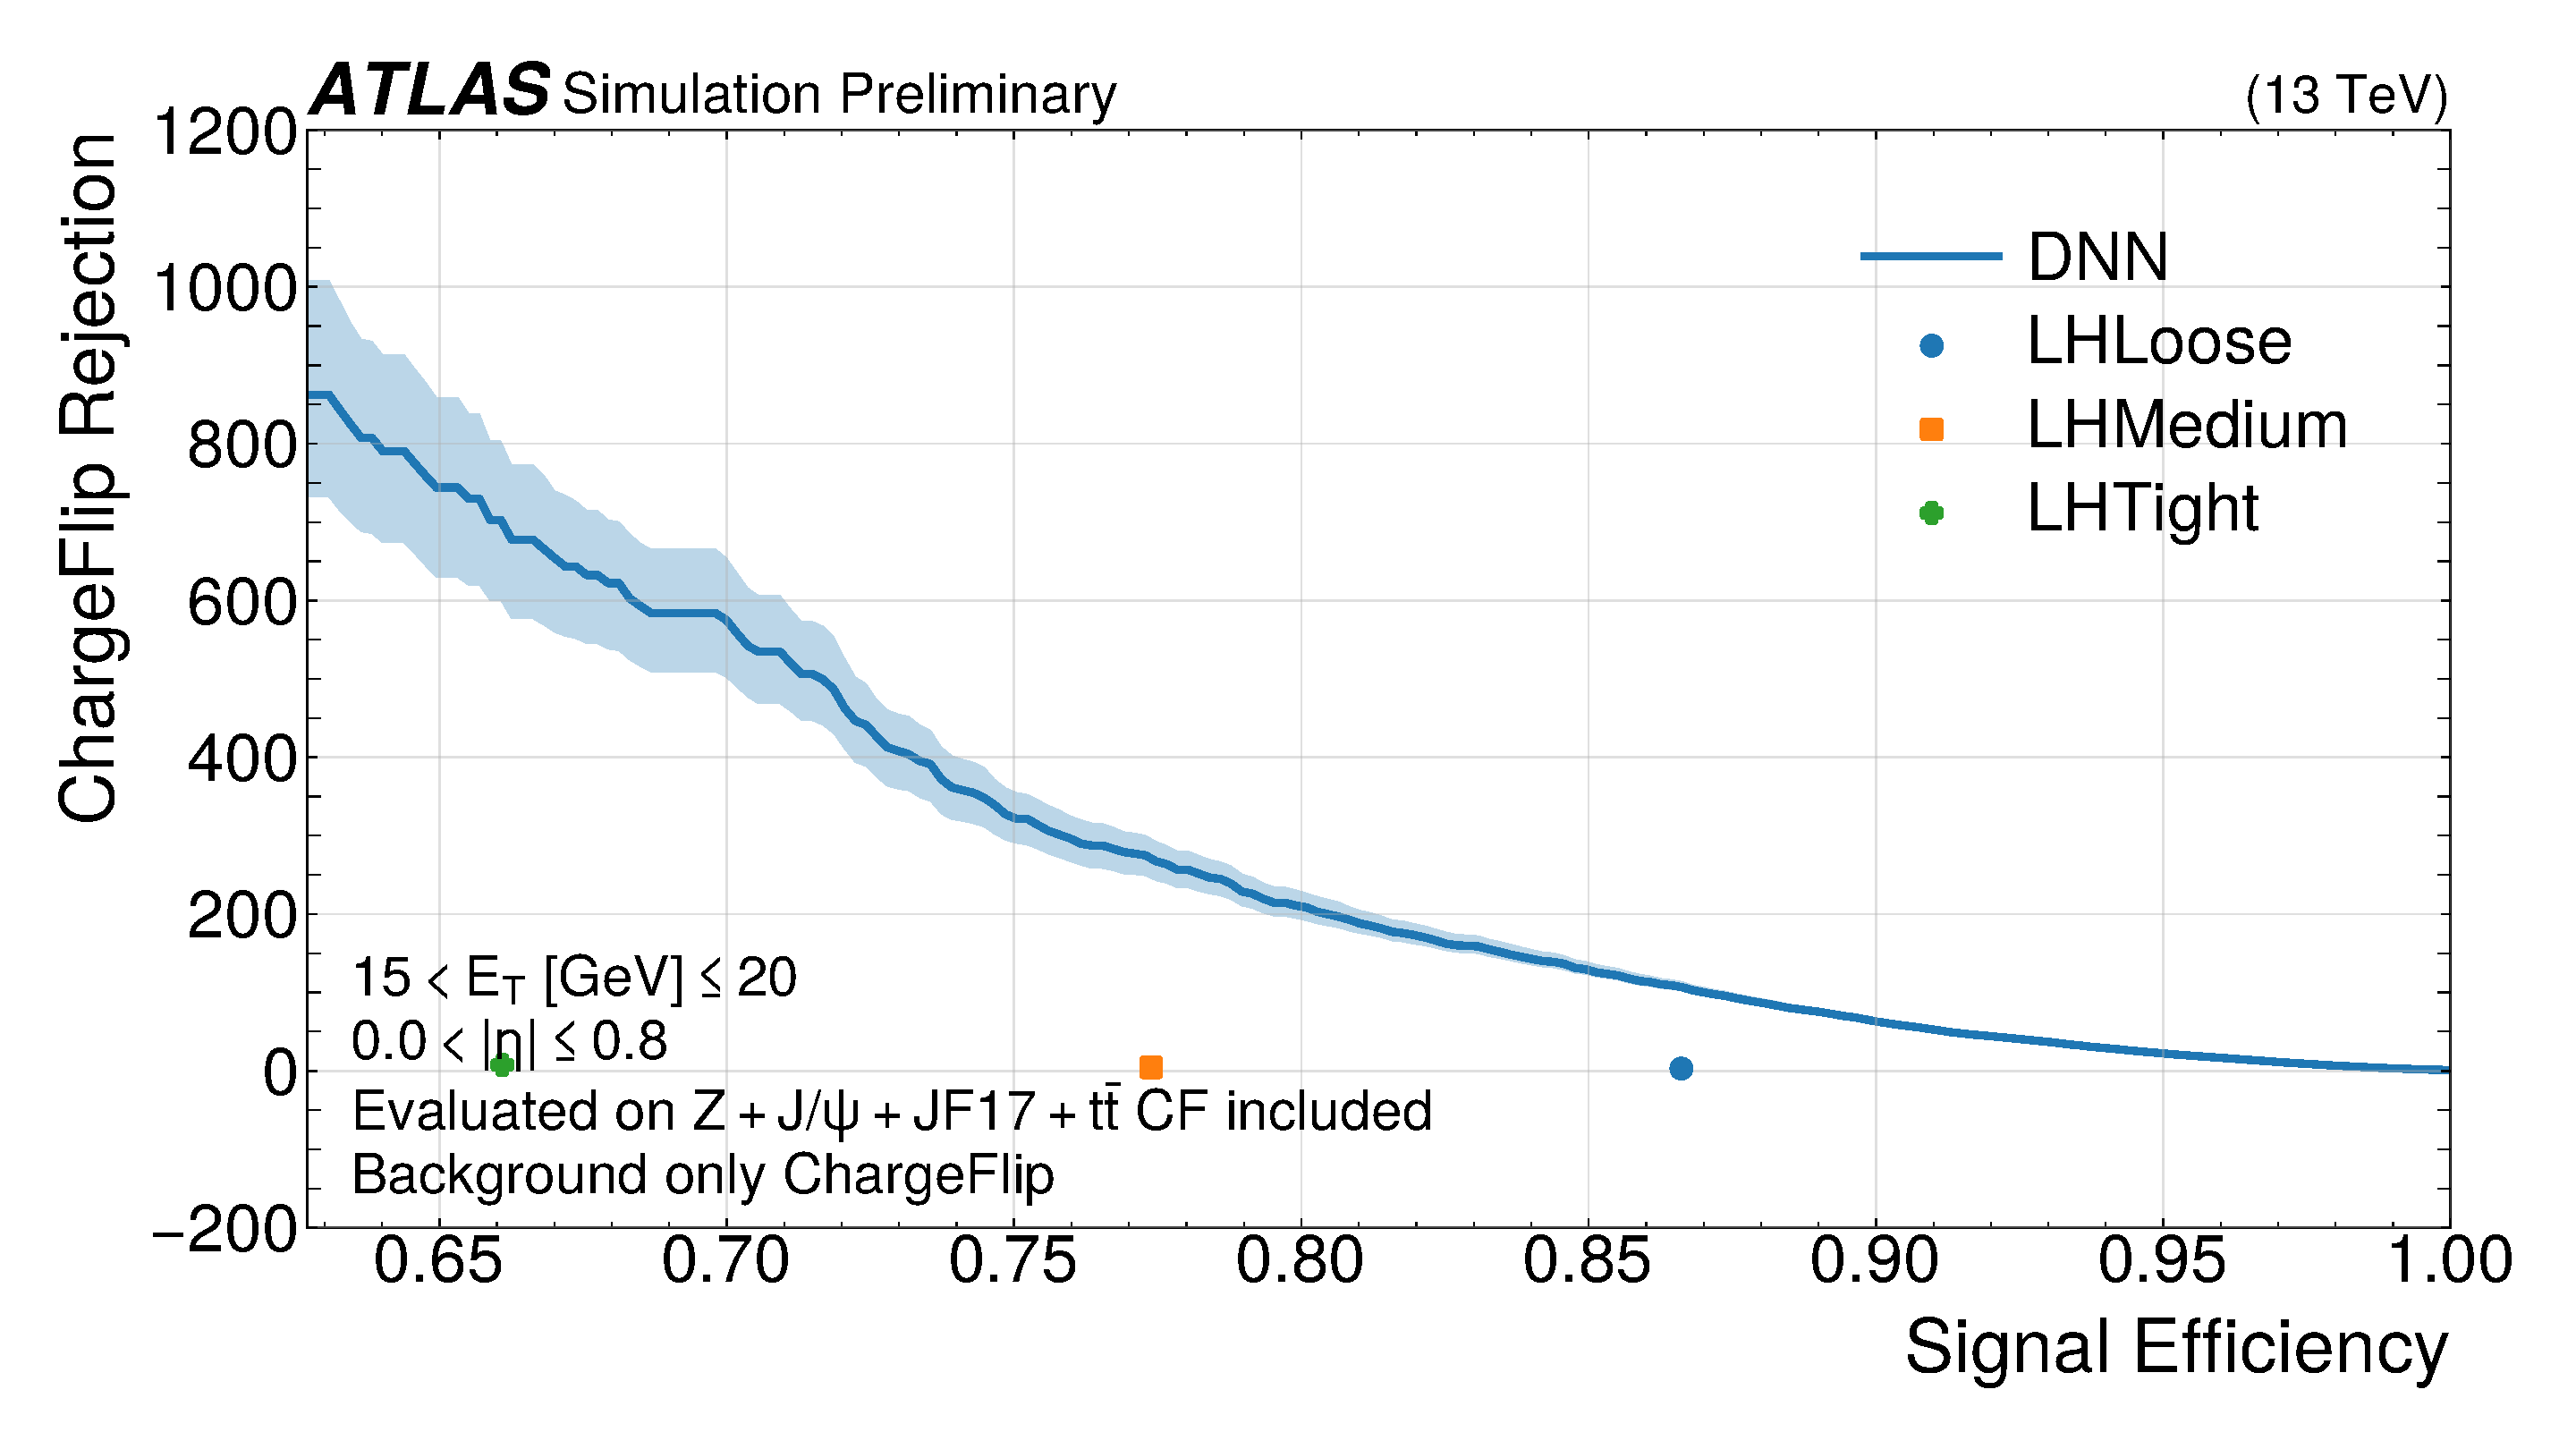
\includegraphics[width=\linewidth]{ROC/15_20_0p0_0p8/binnedROCCurveChargeFlip_et15_20_eta0.0_0.8.pdf}
    \caption{}
    \label{fig:roc_hf}
  \end{subfigure}

  \caption{Rechazo de fondo frente a eficiencia de señal (curvas ROC) para electrones primarios frente a:
  (a) fondo de LFH  ,
  y (e) electrones de \texit{Charge-flips}.
  Las curvas se muestran para un bin representativo de $(E_{T}, |\eta|)$, y las incertidumbres estadísticas de cada rechazo de fondo se indican como bandas.}
  \label{fig:roc_mainbkg}
\end{figure}

Finalmente, se presentan las medidas de eficiencia con el método \textit{tag-and-probe} en $Z\to ee$ y $J/\psi\to ee$~\cite{latest_electron_paper_2024}. Estas medidas permiten derivar factores de escala (SF) en función de $E_T$ y $\eta$, corrigiendo posibles diferencias entre datos y simulación MC. Las eficiencias de identificación obtenidas con el DNN muestran una estabilidad notable a lo largo del rango cinemático y frente al número de vértices primarios $\mu$, manteniéndose en muy buen acuerdo entre datos y MC, con SF cercanos a la unidad en todo el espacio de fase.  
En términos de eficiencia de identificación de señal, tanto el método LH como el DNN alcanzan resultados muy similares, como era esperado al utilizar las mismas efiencias pre-definidas como objetivo a la hora definir los distintos \textit{Working Points} de identificación. Sin embargo, las diferencias se hacen patentes en la capacidad de rechazo de fondo. En medidas realizadas en simulaciones MC, el DNN logra incrementos de hasta un 30-40\% mayormente en la supresión de fondos de LFH, en rangos bajos e intermedios de \et. Estas diferencias se traducen, al evaluar en datos la significancia en la identificación de señal sobre el rechazo de fondo, en una ganancia sistemática del DNN respecto al LH en todos los bins de $(E_T,\eta)$, con aumentos típicos de un 10-15\% en la significancia global.
% ================= Figura 1: eficiencias vs eta en 4 bins de pT =================
\begin{figure}[h]
  \centering

  \begin{subfigure}[b]{0.48\textwidth}
    \centering
    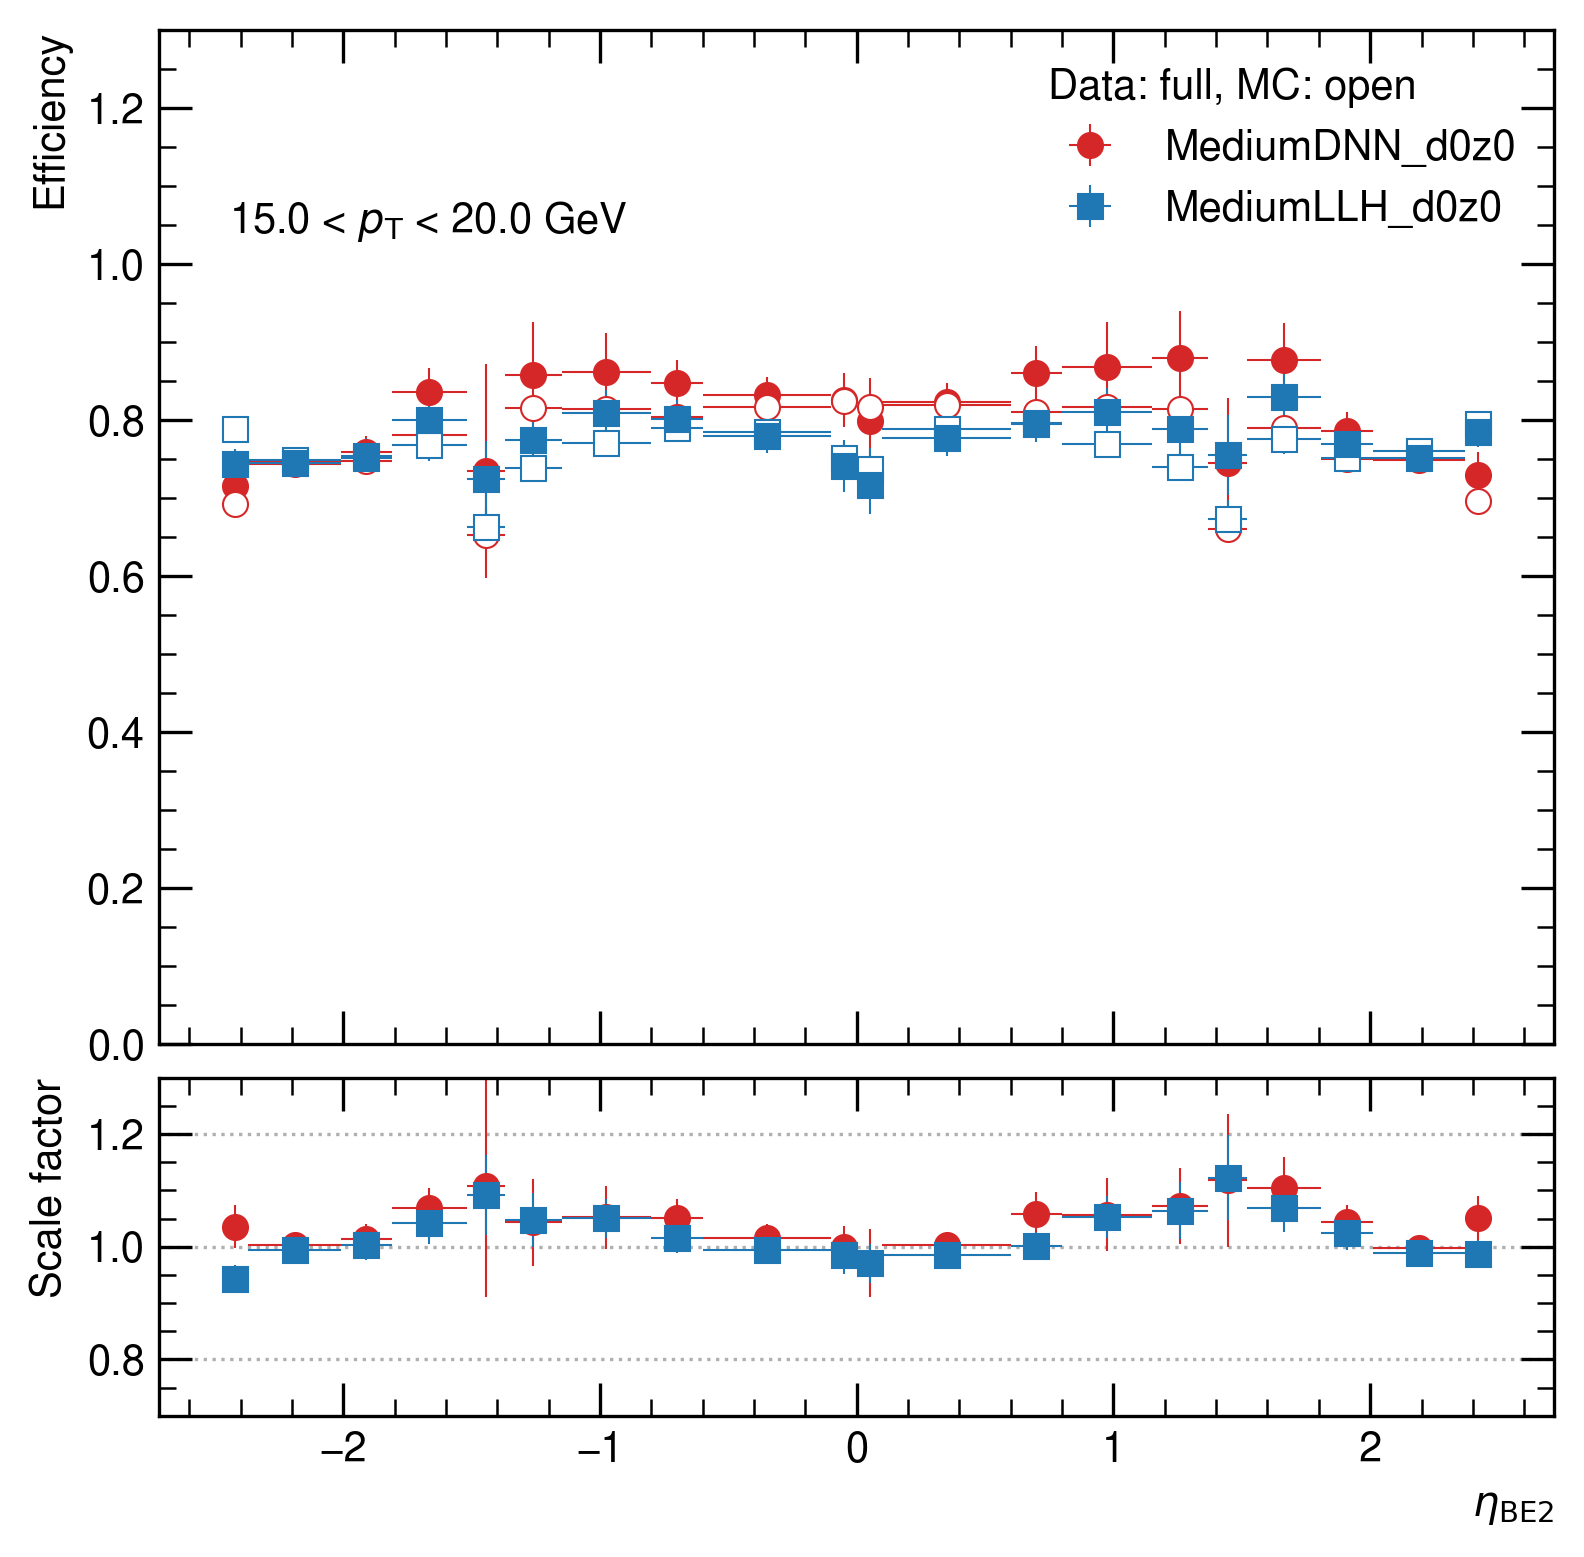
\includegraphics[width=\linewidth]{electron_eff_plots/DNN_ID_effs/DNNID_LH_eff_vs_primary_cluster_be2_eta_for_pt_15p0_20p0.png}
    \caption{$15 < p_{\mathrm{T}} < 20$~GeV}
    \label{fig:eff_dnn_lh_ptbin1}
  \end{subfigure}
  \hfill
  \begin{subfigure}[b]{0.48\textwidth}
    \centering
    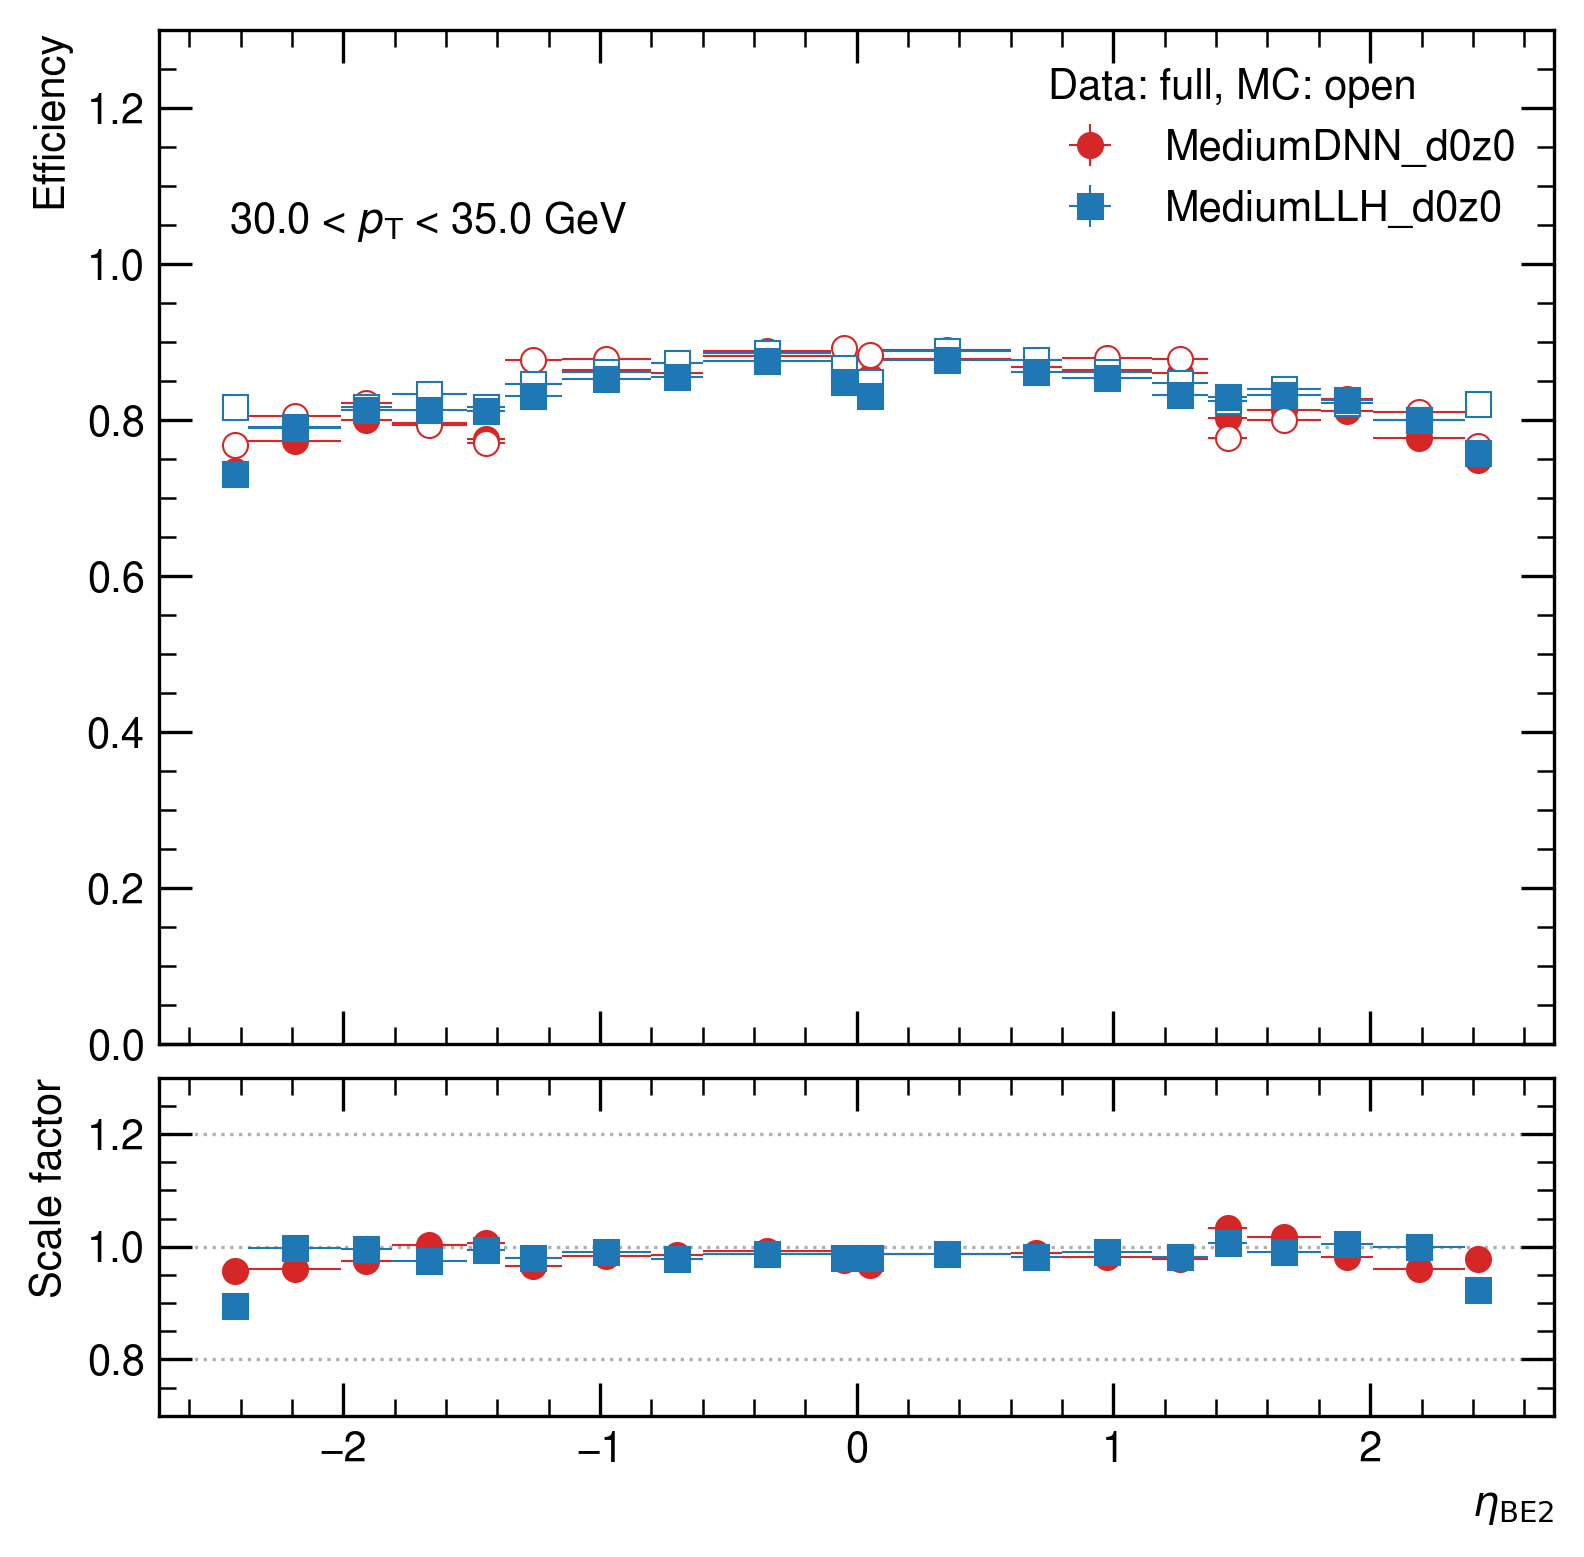
\includegraphics[width=\linewidth]{electron_eff_plots/DNN_ID_effs/DNNID_LH_eff_vs_primary_cluster_be2_eta_for_pt_30p0_35p0.png}
    \caption{$20 < p_{\mathrm{T}} < 30$~GeV}
    \label{fig:eff_dnn_lh_ptbin2}
  \end{subfigure}

  \vspace{0.5cm}

  \begin{subfigure}[b]{0.48\textwidth}
    \centering
    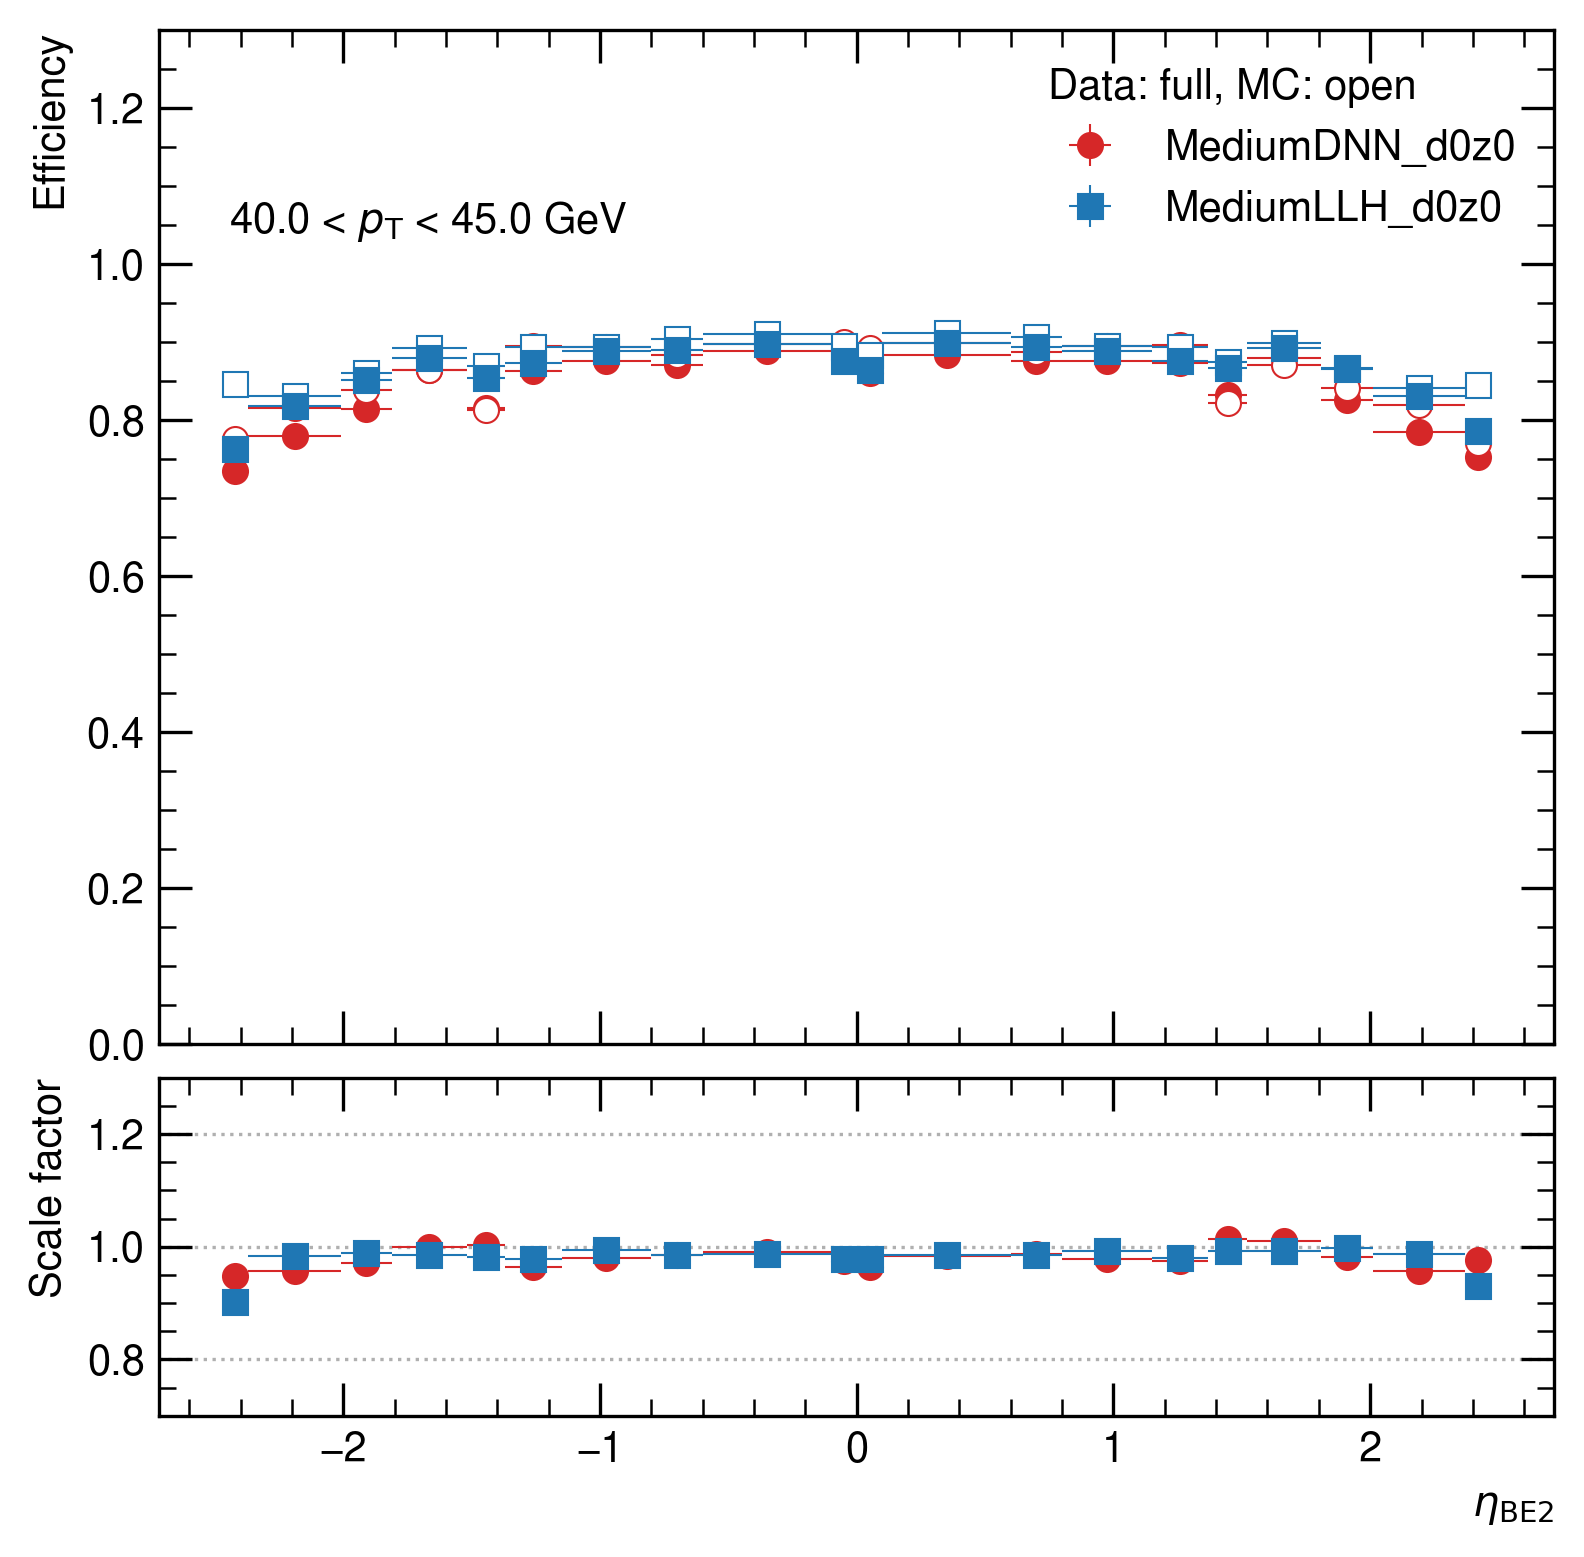
\includegraphics[width=\linewidth]{electron_eff_plots/DNN_ID_effs/DNNID_LH_eff_vs_primary_cluster_be2_eta_for_pt_40p0_45p0.png}
    \caption{$30 < p_{\mathrm{T}} < 40$~GeV}
    \label{fig:eff_dnn_lh_ptbin3}
  \end{subfigure}
  \hfill
  \begin{subfigure}[b]{0.48\textwidth}
    \centering
    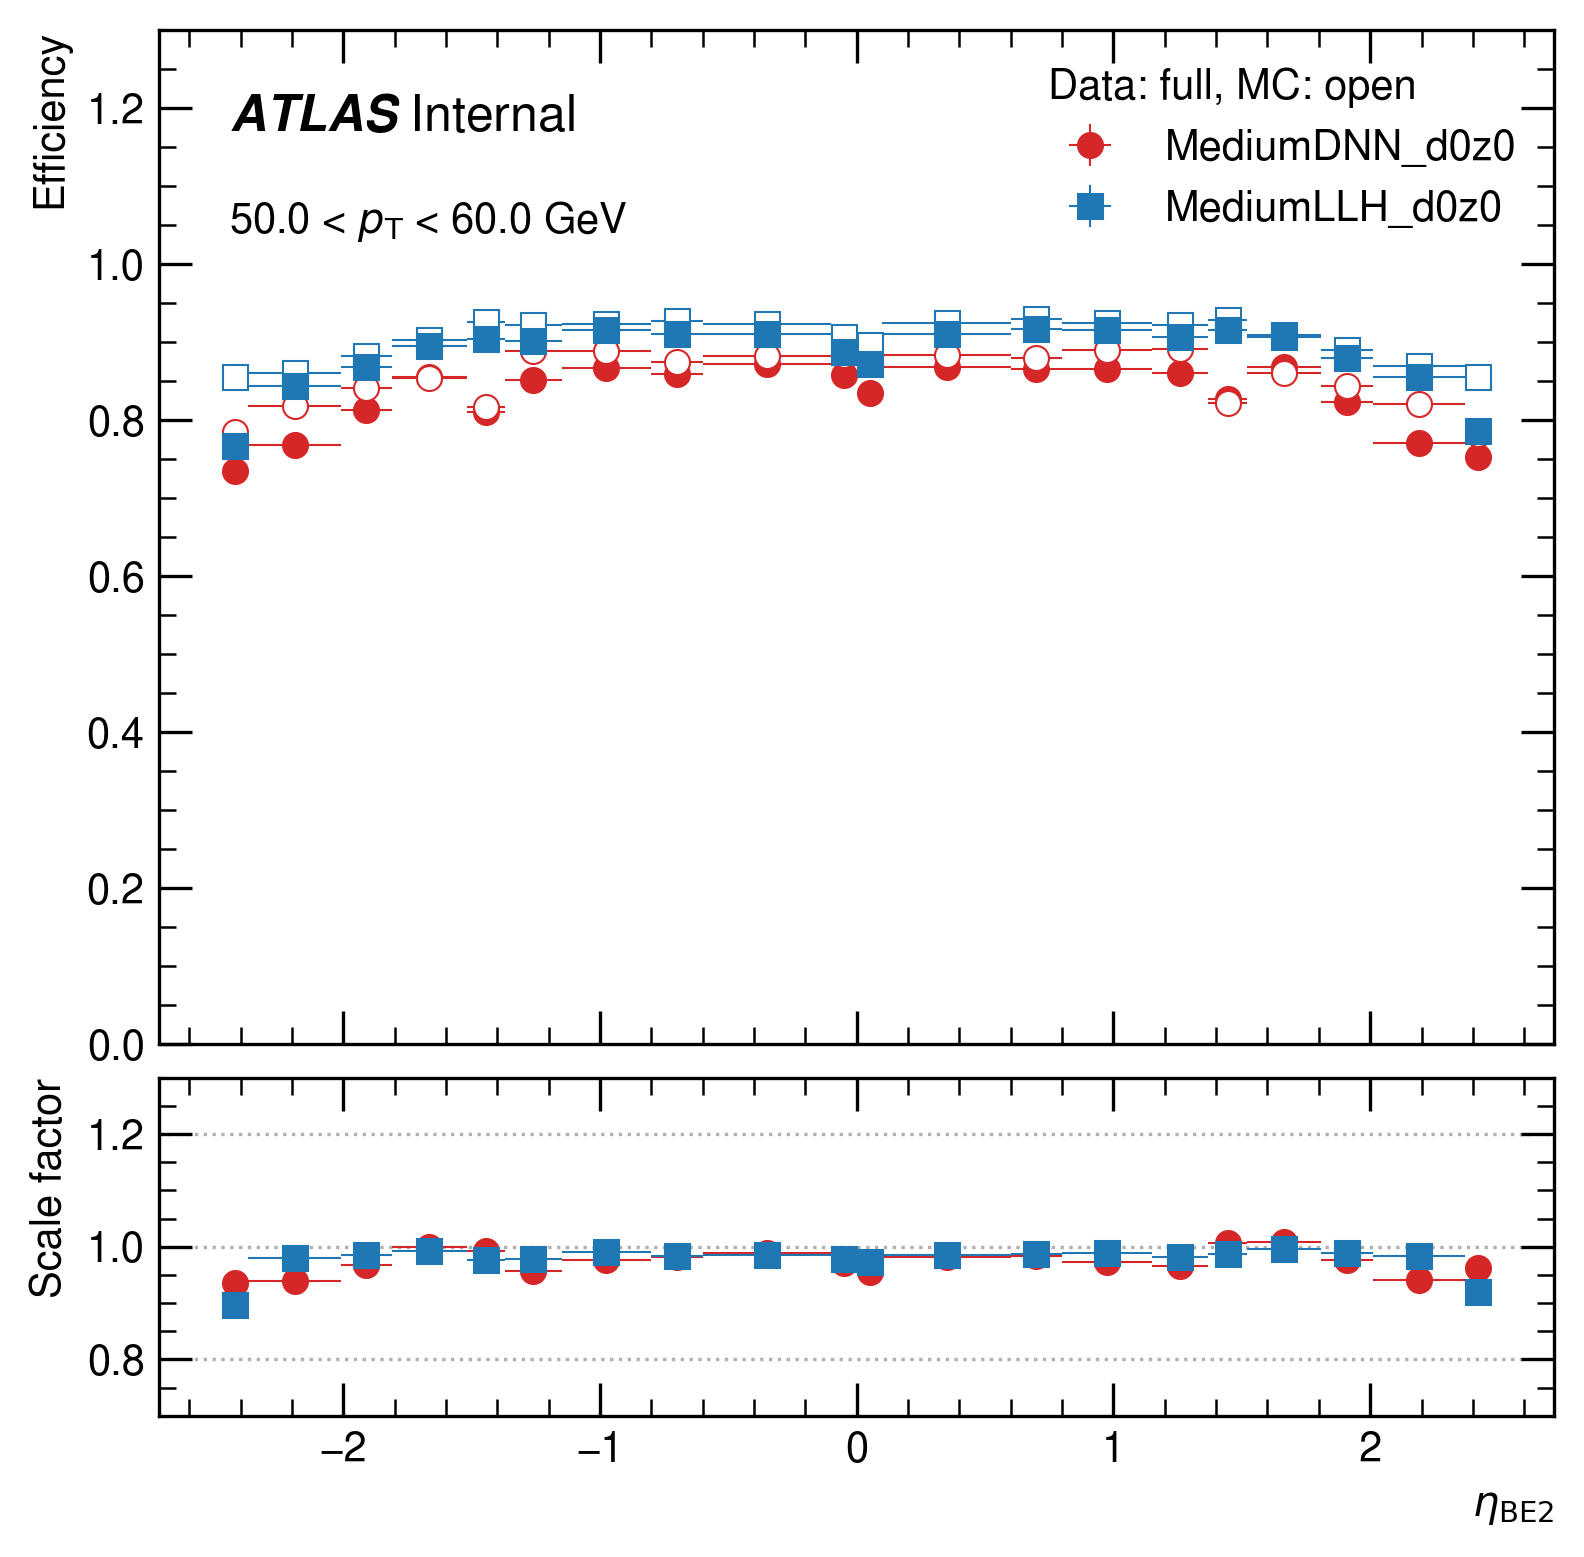
\includegraphics[width=\linewidth]{electron_eff_plots/DNN_ID_effs/DNNID_LH_eff_vs_primary_cluster_be2_eta_for_pt_50p0_60p0.png}
    \caption{$40 < p_{\mathrm{T}} < 45$~GeV}
    \label{fig:eff_dnn_lh_ptbin4}
  \end{subfigure}

  \caption{
    Comparación entre las eficiencias de identificación de señal medidas con DNN y con LH utilizando el \textit{working point} Medium, 
    tanto en datos como en MC, junto con los factores de escala, para el menú DNN ID-only. 
    Las eficiencias se muestran en función de $\eta$ en cuatro bins representativos de $p_{\mathrm{T}}$. 
    Las barras de error incluyen todas las incertidumbres estadísticas y sistemáticas.}
  \label{fig:eff_sfs_dnn_vs_lh_eta_4ptbins}
\end{figure}


% ================= Figura 2: eficiencias vs pT en 4 bins de eta =================
\begin{figure}[h]
  \centering

  \begin{subfigure}[b]{0.48\textwidth}
    \centering
    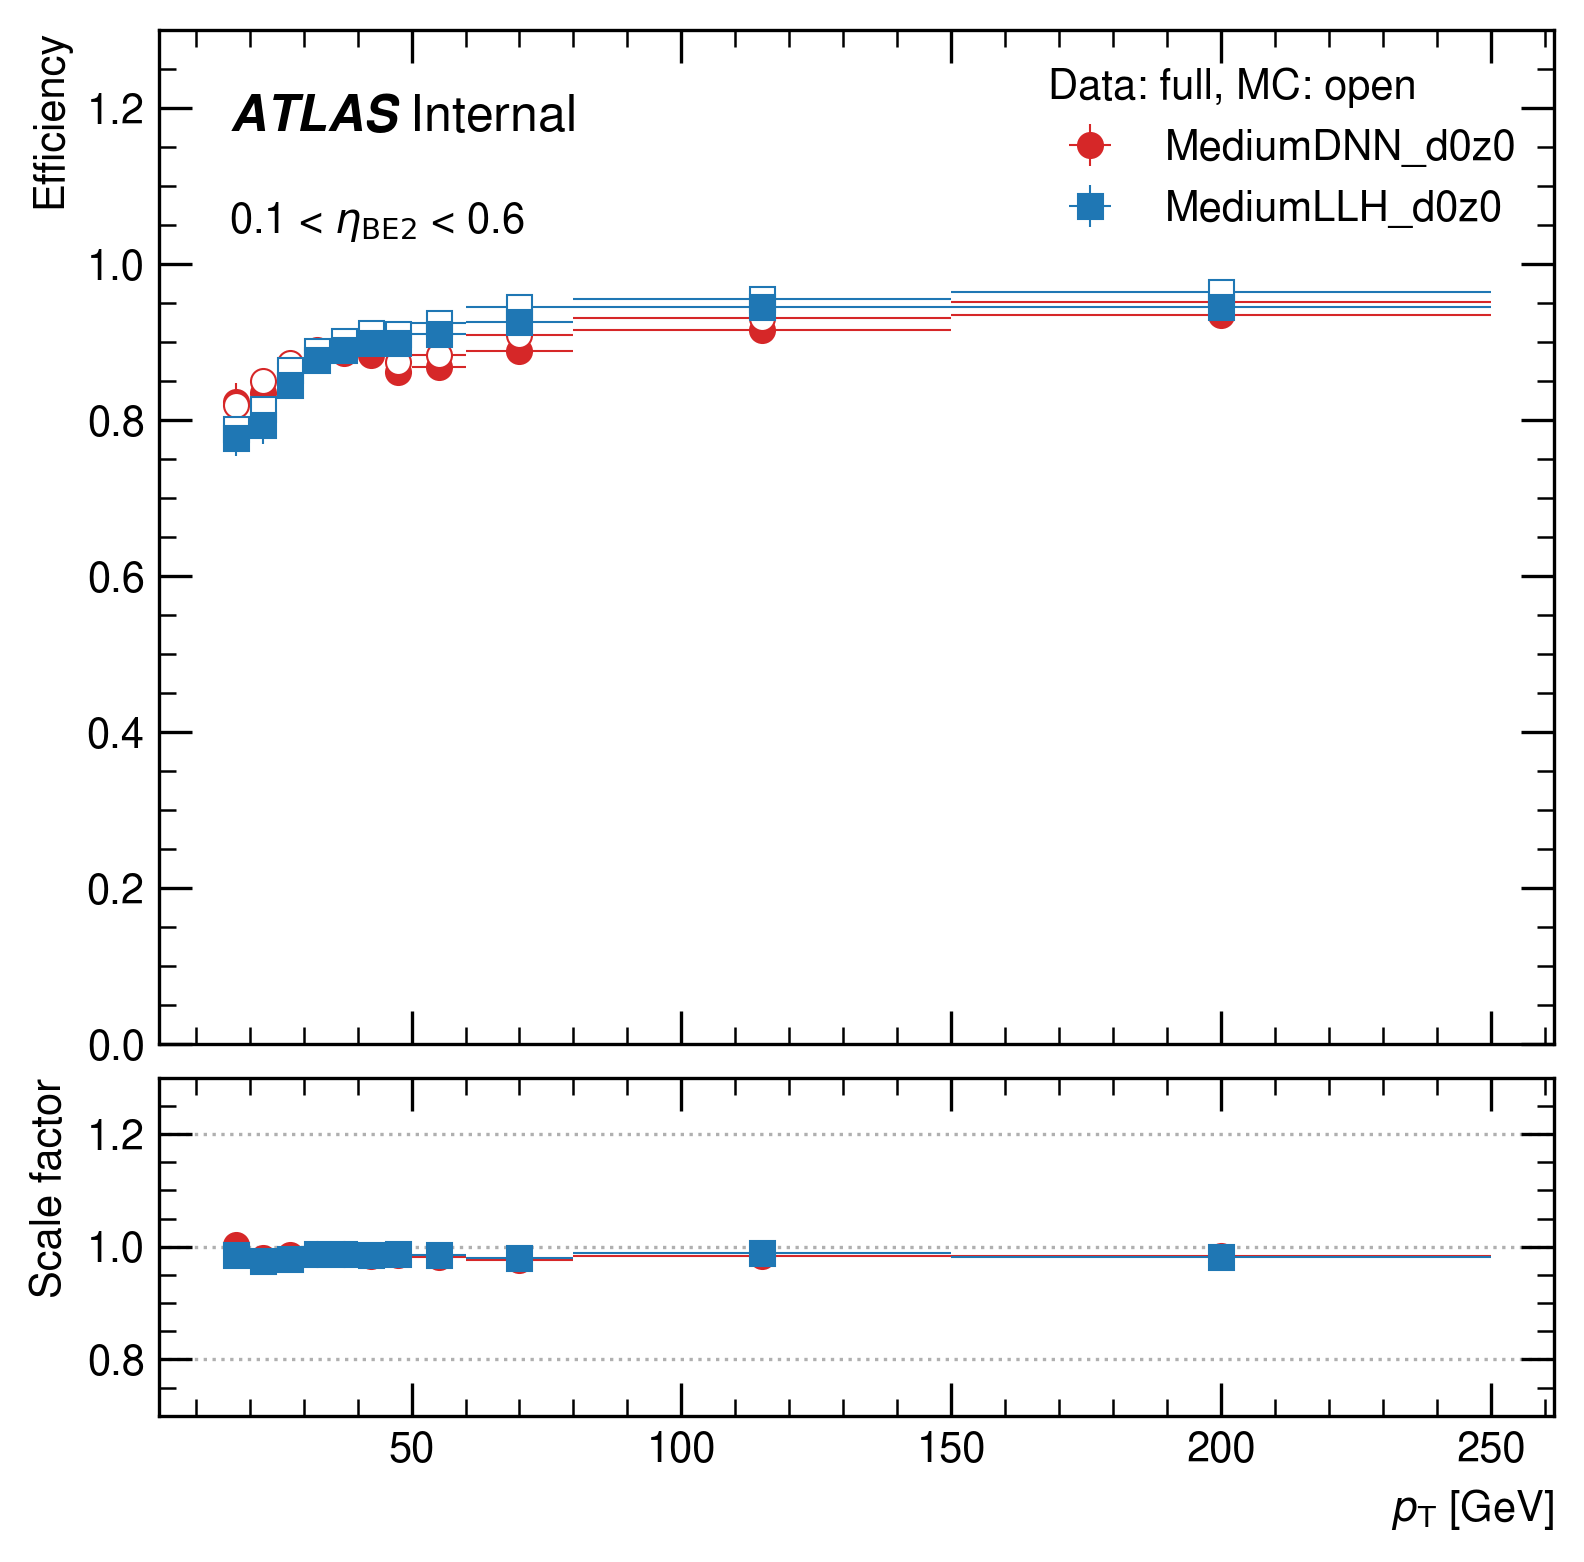
\includegraphics[width=\linewidth]{electron_eff_plots/DNN_ID_effs/DNNID_LH_eff_vs_pt_for_primary_cluster_be2_eta_0p1_0p6.png}
    \caption{$0.1 < \eta < 0.6$}
    \label{fig:eff_dnn_lh_etabin1}
  \end{subfigure}
  \hfill
  \begin{subfigure}[b]{0.48\textwidth}
    \centering
    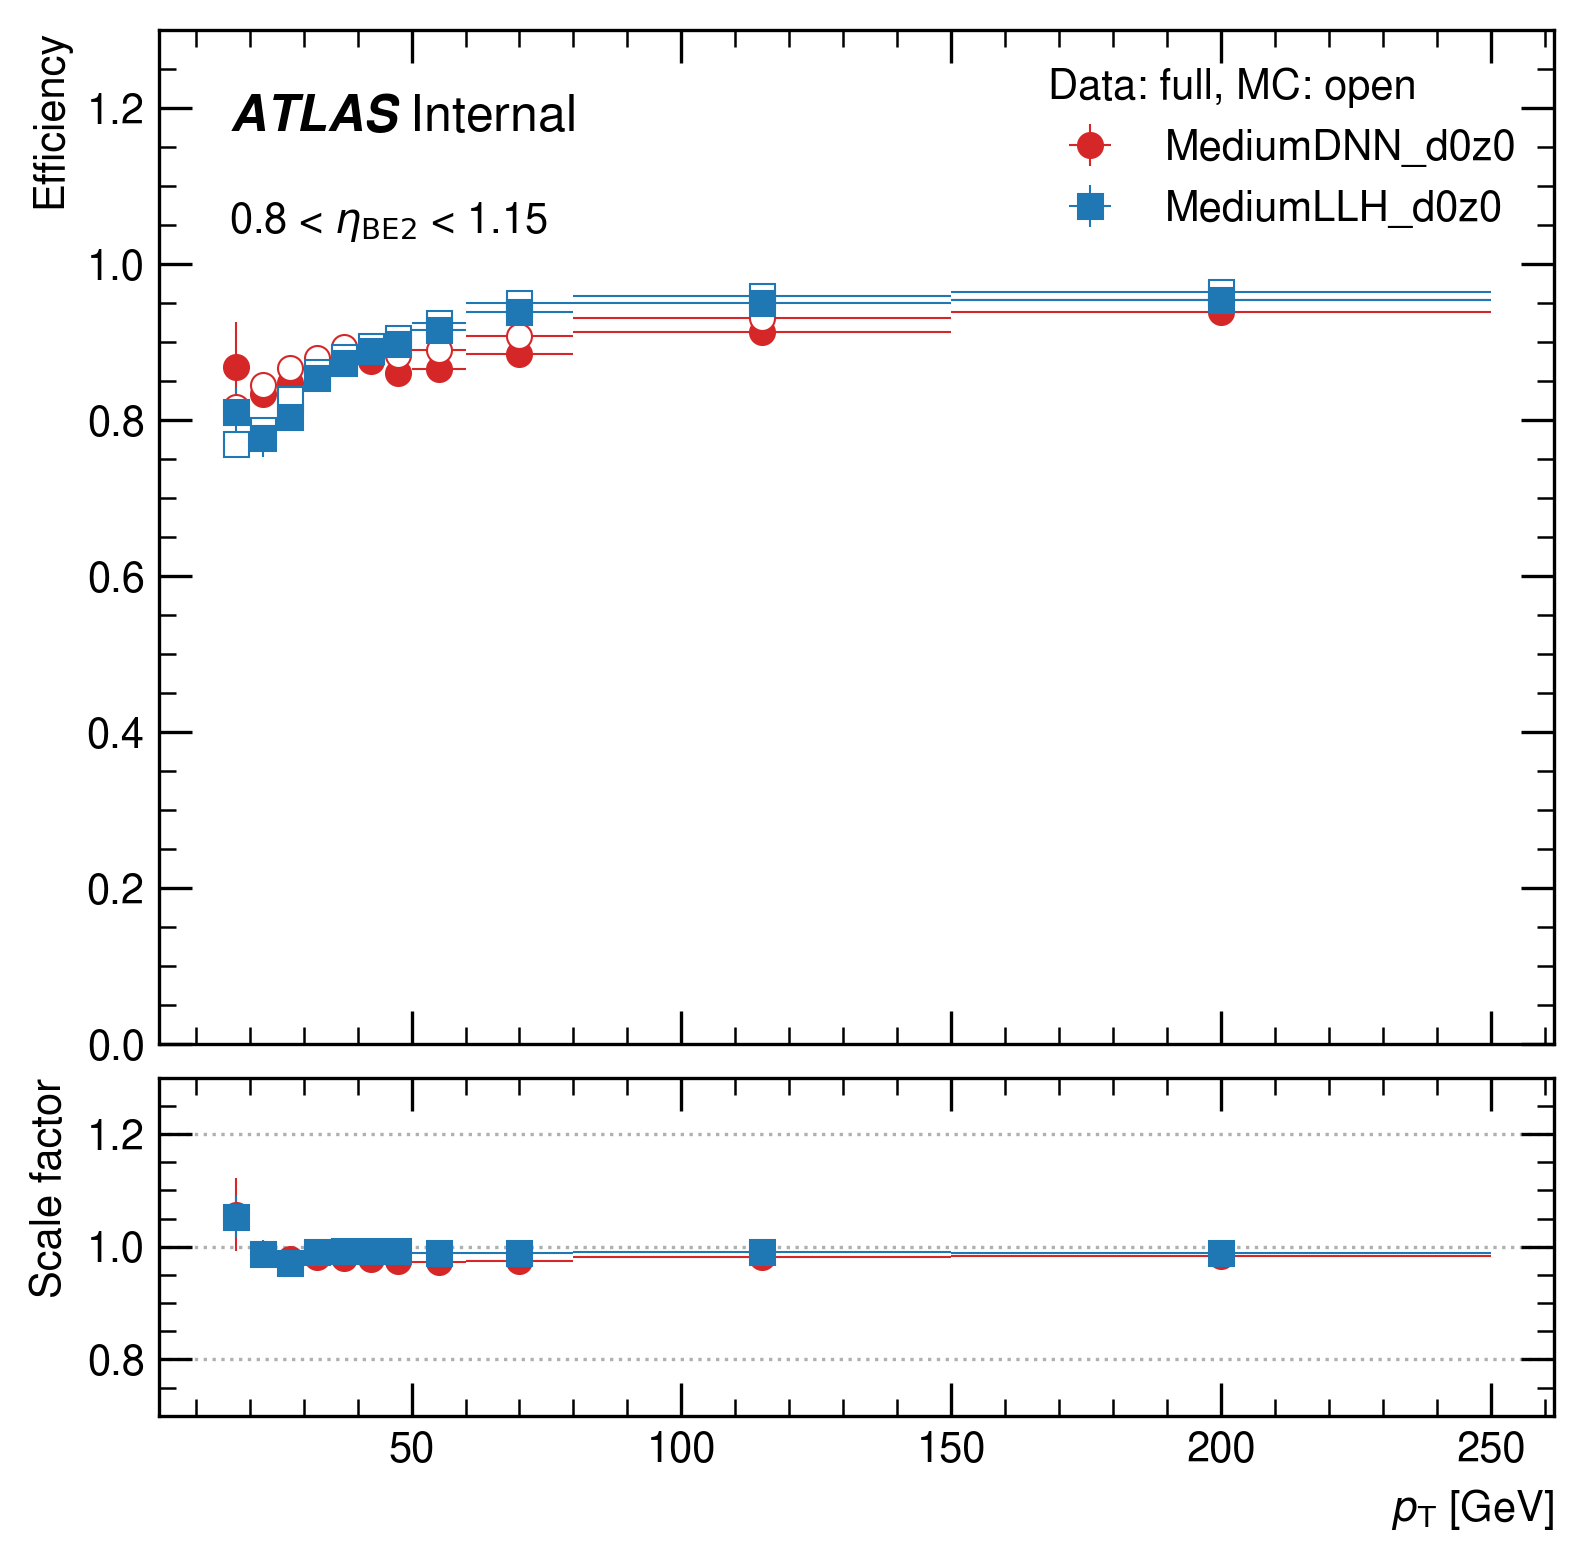
\includegraphics[width=\linewidth]{electron_eff_plots/DNN_ID_effs/DNNID_LH_eff_vs_pt_for_primary_cluster_be2_eta_0p8_1p15.png}
    \caption{$0.6 < \eta < 1.0$}
    \label{fig:eff_dnn_lh_etabin2}
  \end{subfigure}

  \vspace{0.5cm}

  \begin{subfigure}[b]{0.48\textwidth}
    \centering
    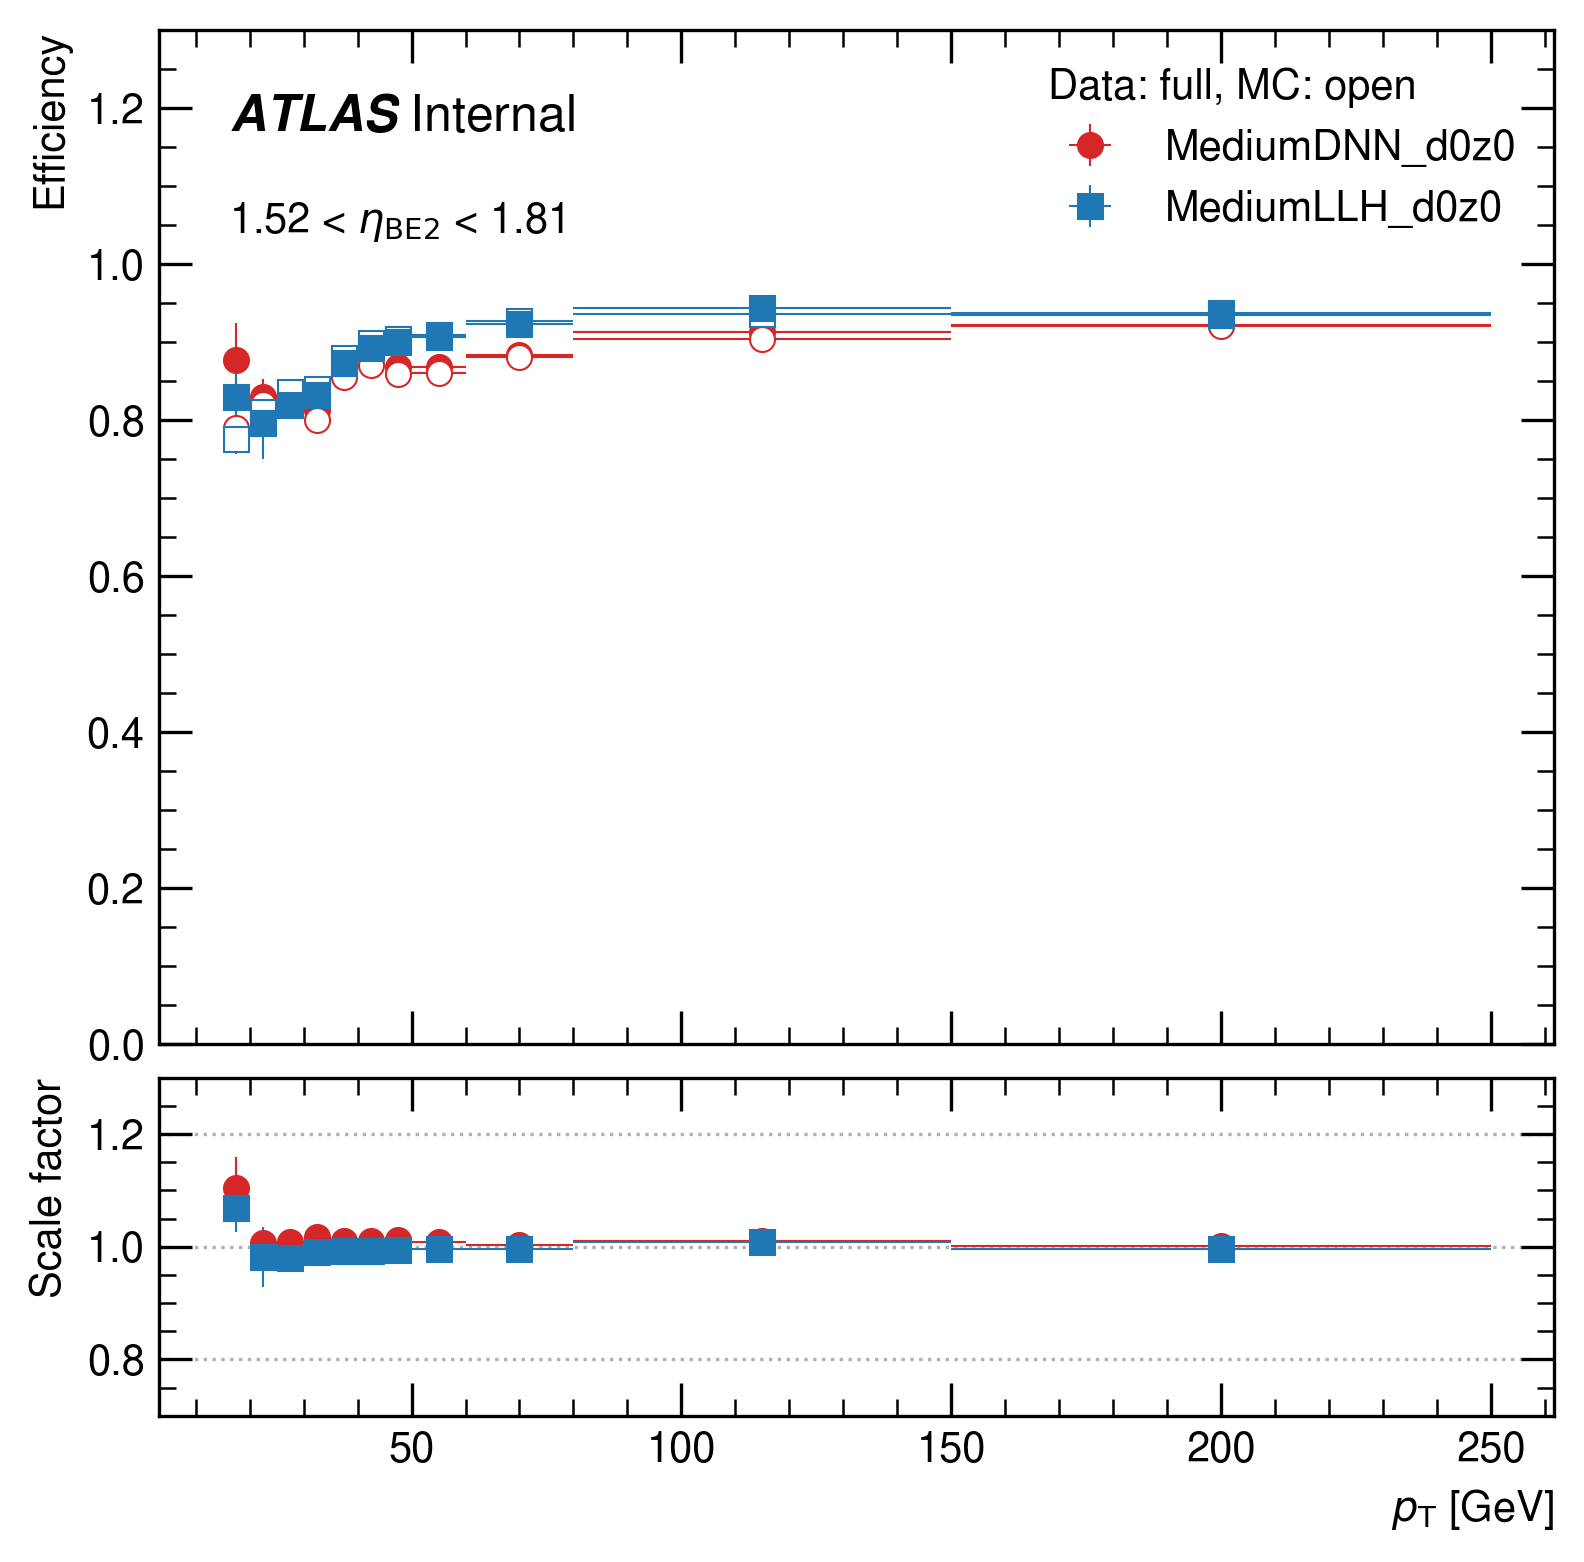
\includegraphics[width=\linewidth]{electron_eff_plots/DNN_ID_effs/DNNID_LH_eff_vs_pt_for_primary_cluster_be2_eta_1p52_1p81.png}
    \caption{$1.0 < \eta < 1.37$}
    \label{fig:eff_dnn_lh_etabin3}
  \end{subfigure}
  \hfill
  \begin{subfigure}[b]{0.48\textwidth}
    \centering
    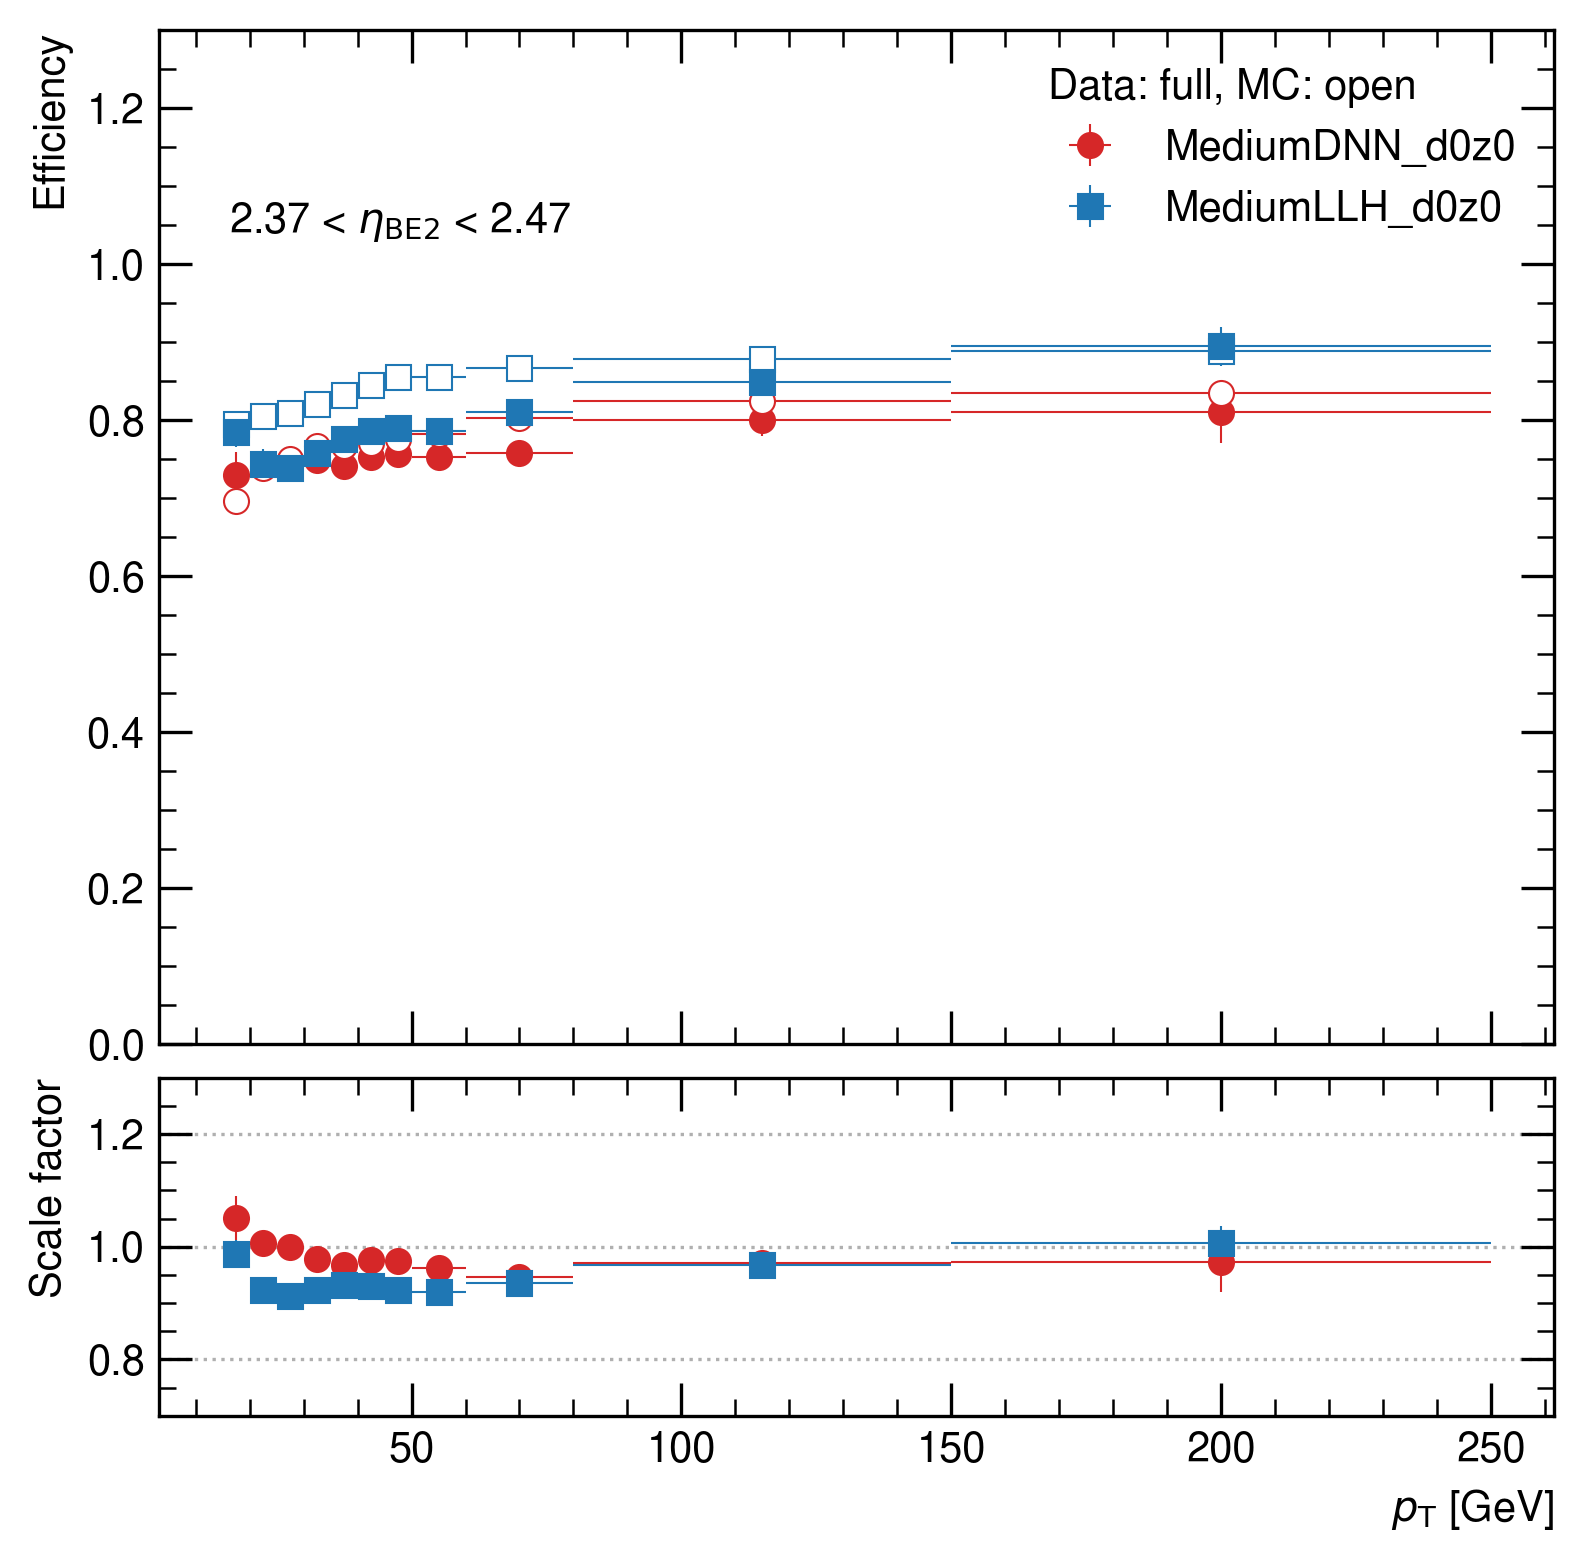
\includegraphics[width=\linewidth]{electron_eff_plots/DNN_ID_effs/DNNID_LH_eff_vs_pt_for_primary_cluster_be2_eta_2p37_2p47.png}
    \caption{$1.52 < \eta < 1.81$}
    \label{fig:eff_dnn_lh_etabin4}
  \end{subfigure}

  \caption{
    Comparación entre las eficiencias de identificación de señal medidas con DNN y con LH utilizando el \textit{working point} Medium, 
    tanto en datos como en MC, junto con los factores de escala, para el menú DNN ID-only. 
    Las eficiencias se muestran en función de $p_{\mathrm{T}}$ en cuatro bins representativos de $\eta$. 
    Las barras de error incluyen todas las incertidumbres estadísticas y sistemáticas.}
  \label{fig:eff_sfs_dnn_vs_lh_pt_4etabins}
\end{figure}

\begin{figure}[h]
  \centering

  \begin{subfigure}{0.48\textwidth}
    \centering
    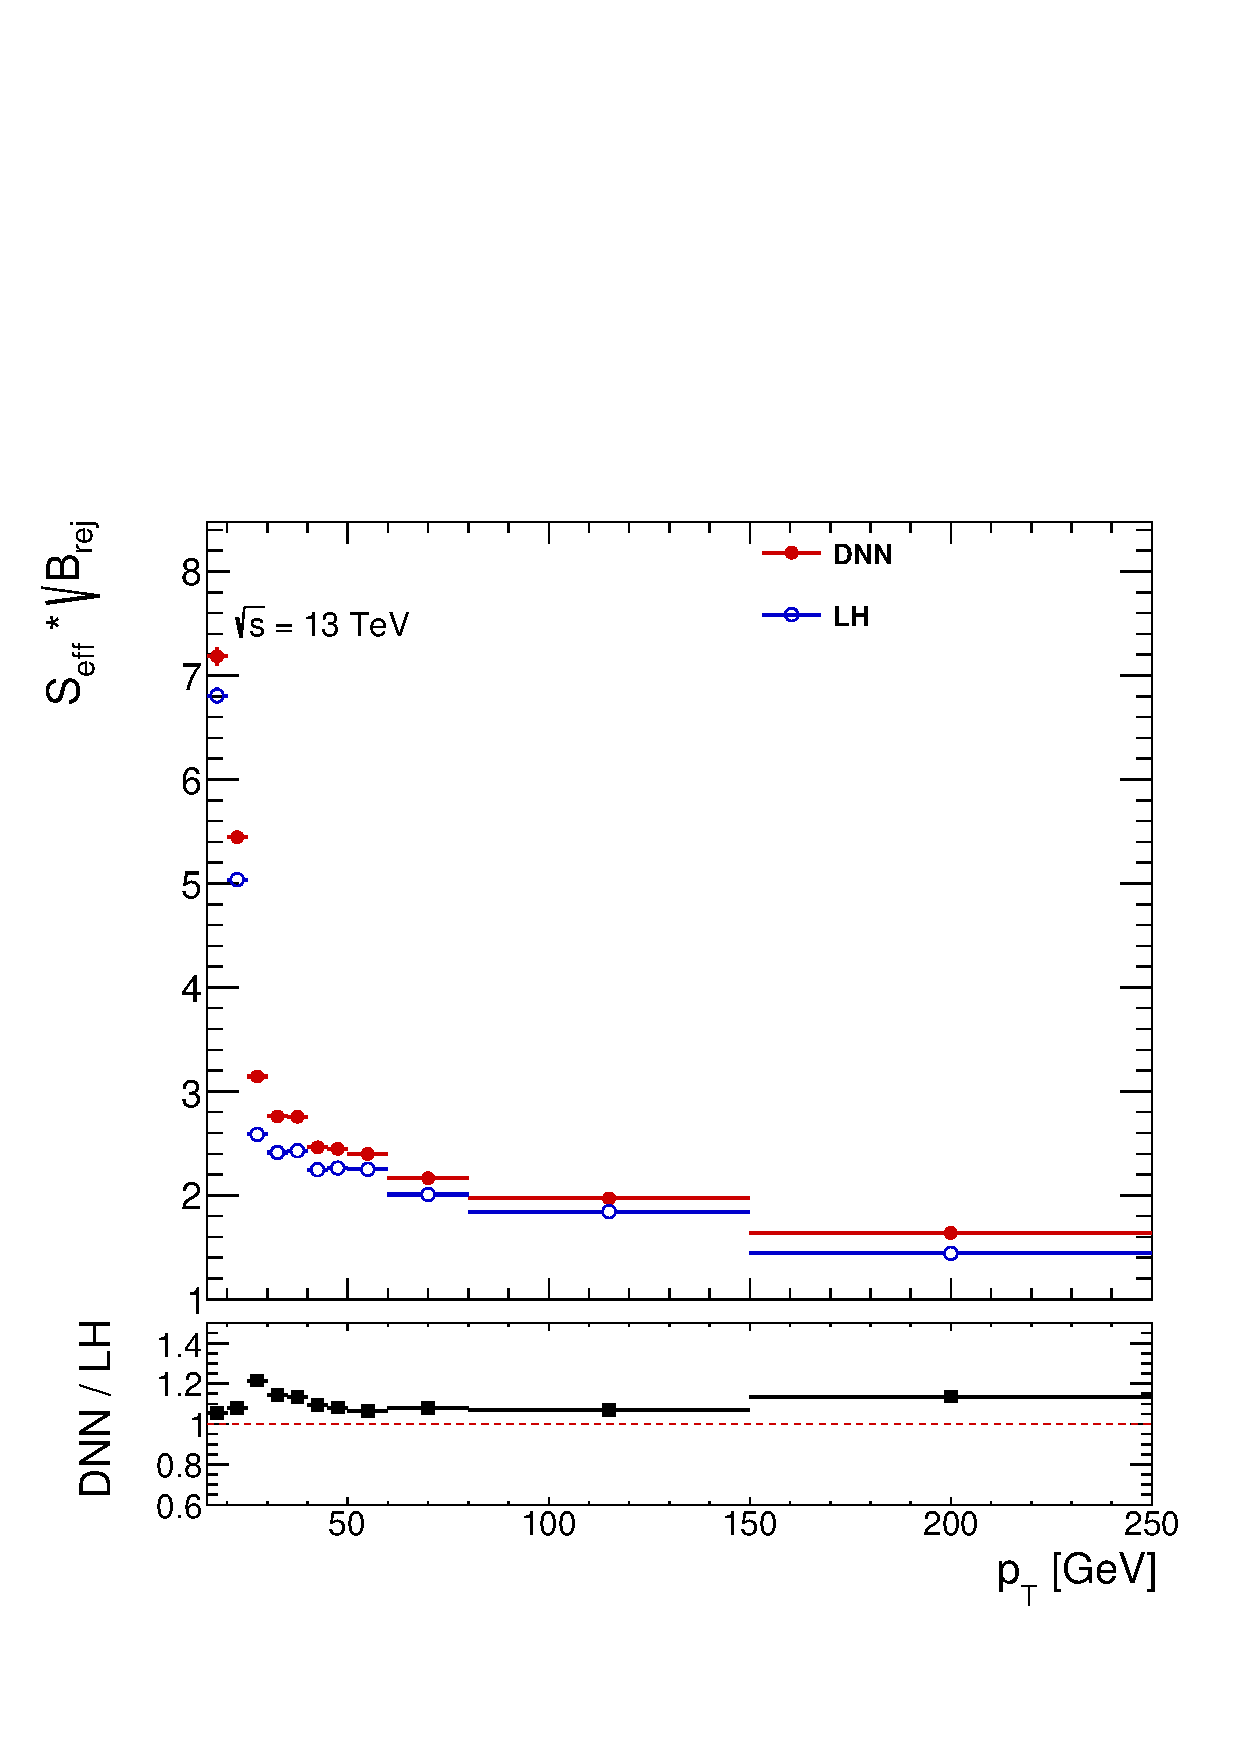
\includegraphics[width=\linewidth]{electron_eff_plots/significance_data/significance_vs_pt_etaBin_0.60_0.80.pdf}
    \caption{\small{Significance vs $E_{\mathrm{T}}$, $|\eta|\in[1.37,1.52]$.}}
    \label{fig:significance_vs_pt_etaBin}
  \end{subfigure}\hfill
  \begin{subfigure}{0.48\textwidth}
    \centering
    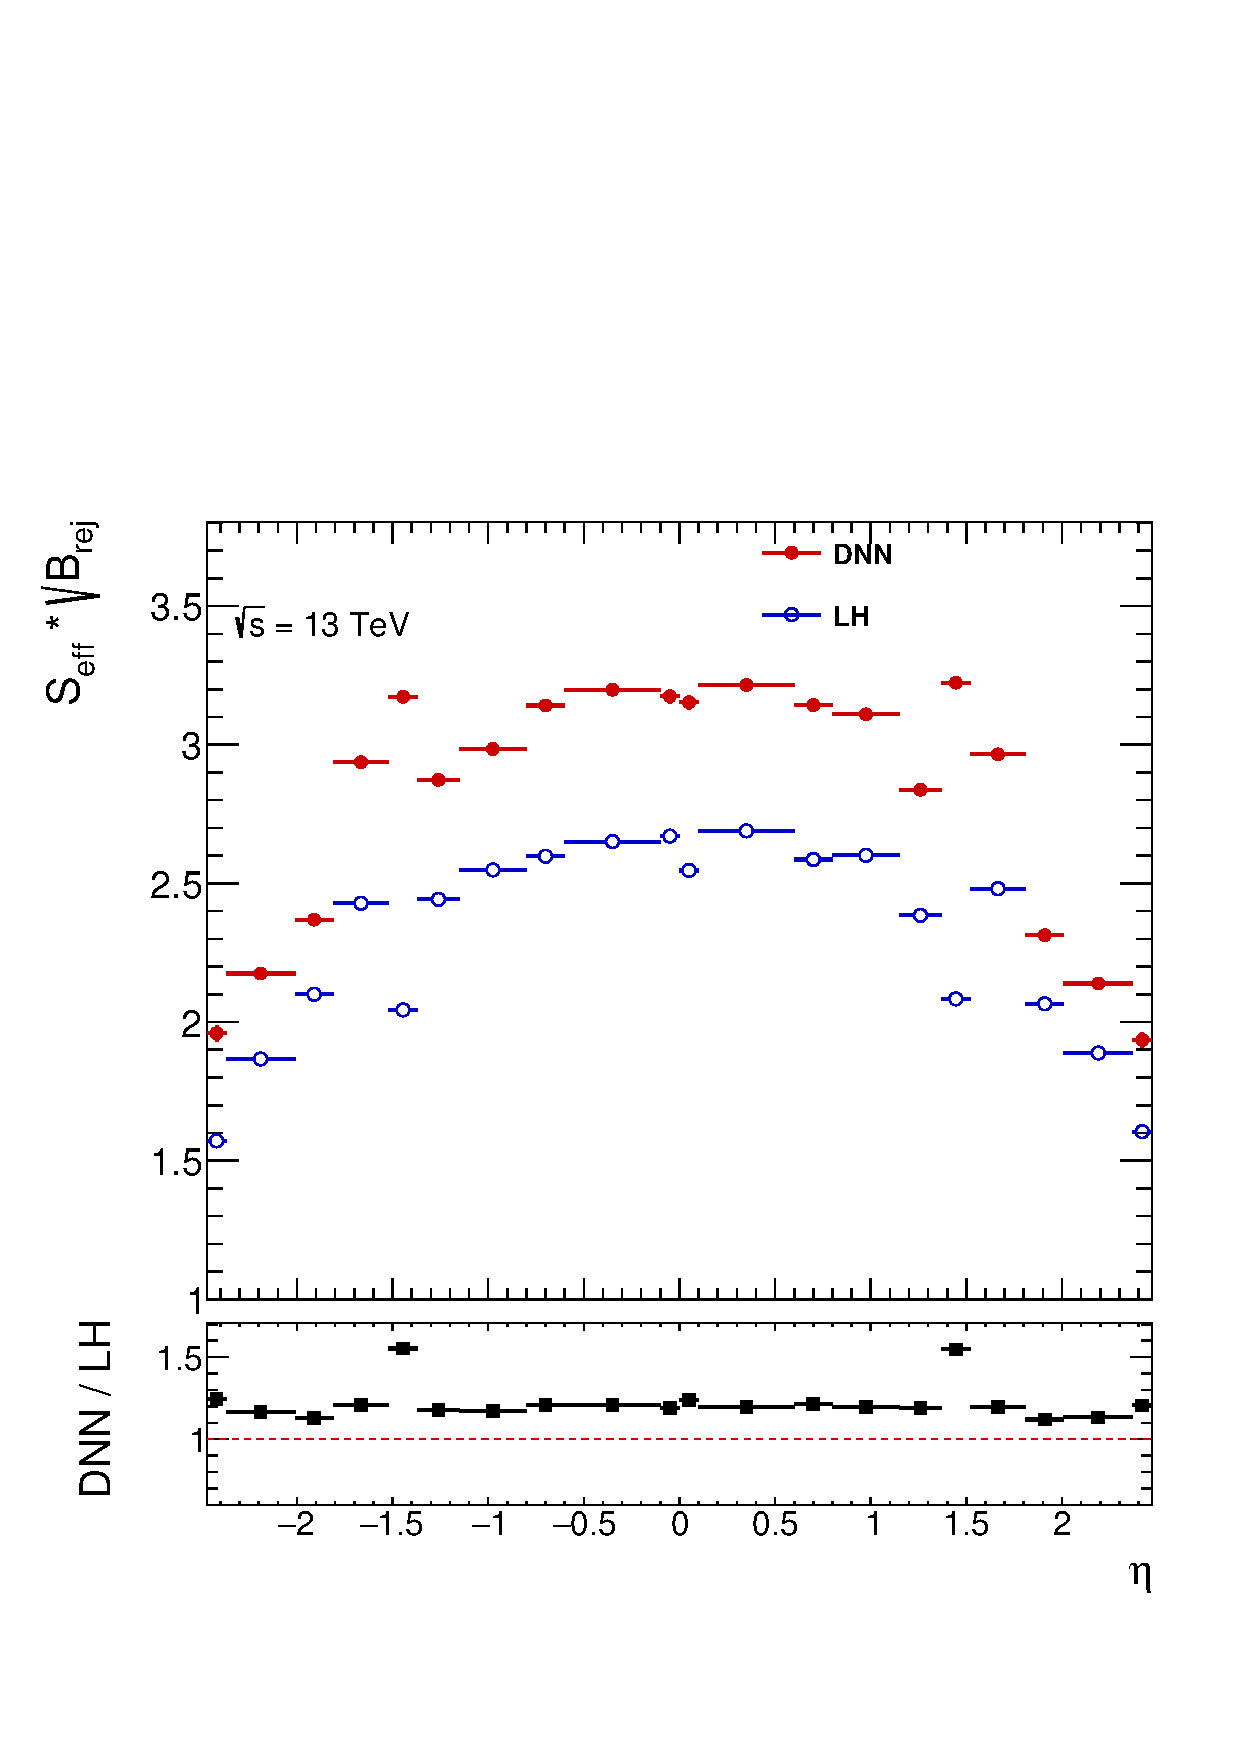
\includegraphics[width=\linewidth]{electron_eff_plots/significance_data/significance_vs_eta_ptBin_25_30.pdf}
    \caption{\small{Significance vs $|\eta|$, $E_{\mathrm{T}}\in[25,35]$~GeV.}}
    \label{fig:significance_vs_eta_ptBin}
  \end{subfigure}

  \caption{Estimación de la significancia $S_{\mathrm{eff}} \times \sqrt{\mathrm{Bkg}_{\mathrm{rej}}}$ 
  calculada en datos para los menús de identificación de DNN y LH. 
  Los resultados se muestran en función de $E_{\mathrm{T}}$ para $|\eta|$ inclusiva (a) and en función de $|\eta|$ inclusivos en $E_{\mathrm{T}}$ (b).}
  \label{fig:significance_bins}
\end{figure}


En conclusión, el trabajo presentado demuestra que la transición del método LH al DNN en la identificación de electrones supone un salto cualitativo. La estabilidad de las eficiencias y de los factores de escala, combinada con una mejora clara en el rechazo de fondo y en la significancia observada en datos, refuerzan el potencial de este algoritmo para Run~3, donde podría llegar a reemplazar al LH como estrategia nominal en los análisis de ATLAS que dependen de electrones de alta calidad. 

\FloatBarrier

\section*{Medida de la producción de \ttH con \htautau}

La producción asociada de un bosón de Higgs con un par top-antitop (\ttH) constituye la vía más directa para acceder al acoplamiento de Yukawa del quark top. Este proceso aparece a \textit{Tree Level} con una dependencia cuadrática en dicho acoplamiento, lo que le otorga una sensibilidad única. Dado que el Yukawa del top es el mayor del Modelo Estándar, su medida precisa es de especial relevancia: no sólo permite verificar la validez interna del modelo y su estabilidad a energías altas, sino que también abre una ventana privilegiada a posibles efectos de nueva física más allá del Modelo Estándar.  

Por otro lado, el canal de desintegración \(H\to\tau\tau\) aporta una oportunidad complementaria al permitir explorar simultáneamente el acoplamiento del Higgs a leptones de tercera generación. Aunque su tasa de desintegración es relativamente modesta, la sensibilidad conjunta a dos Yukawas diferentes lo convierte en un canal de gran interés. Dentro de este modo, la topología en la que ambos leptones $\tau$ decaen hadrónicamente (\(\tau_{\mathrm{had}}\tau_{\mathrm{had}}\)) ofrece la mayor probabilidad de desintegración, pero también plantea los mayores retos experimentales al considerar que los quarks top también se desintegran hadrónicamente: presencia de múltiples jets y \(b\)-jets en el estado final, ausencia de leptones aislados y fondos dominados por \(\ttbar\)+jets y \(Z\to\tau\tau\)+jets.  

Este análisis de \ttH(\(\tau_{\mathrm{had}}\tau_{\mathrm{had}}\)) se enmarca dentro de la medida global de \(H\to\tau\tau\) en ATLAS, que combina distintos modos de producción y canales de desintegración de los leptones $\tau$, proporcionando así un marco coherente para evaluar la sensibilidad de este proceso frente a otros. Tanto ATLAS como CMS han estudiado este canal en Run-1~\cite{htau_cms_atlas_2016} y en primeras etapas de Run-2, aunque con sensibilidades limitadas y grandes incertidumbres~\cite{2022, Tumasyan_2023}.  

El presente trabajo constituye un paso adelante al introducir técnicas multivariantes más refinadas y una categorización optimizada, extendiendo además el análisis al marco de \textit{Simplified Template Cross Sections} (STXS). Este enfoque permite realizar una medida diferencial de la producción en distintos bins del momento transverso del bosón de Higgs, lo que proporciona una visión más rica y reduce correlaciones en las combinaciones globales. Los resultados obtenidos en este análisis se encuentran junto al resto de modos de producción y canales en la publicación de la Ref.~\cite{differential_htautau}.

El objetivo central del análisis es evaluar la sensibilidad del canal \ttHtt, tratando de mejorar la precisión en la medida de la \textit{signal strength},  
\[
  \mu_{t\bar{t}H} = \frac{\sigma_{t\bar{t}H}\times \mathcal{B}(H \to \tau \tau)}{\sigma^{\text{SM}}_{t\bar{t}H}\times \mathcal{B}^{\text{SM}}_{t\bar{t}H}(H \to \tau \tau)}
\]  

El análisis utiliza la muestra completa de datos de Run-2 de ATLAS, correspondiente a una luminosidad integrada de 140~fb$^{-1}$ a $\sqrt{s}=13$~TeV. La señal objetivo es \(\ttH(\tau_{\mathrm{had}}\tau_{\mathrm{had}})\), mientras que los principales procesos de fondo son \(\ttbar\)+jets, $Z\to\tau\tau$+jets y eventos con múltiples jets provenientes de radiaciones QCD que se reconstruyen erroneamente como \tauhad (\textit{Fakes}). Para la modelización se emplean simulaciones Monte Carlo, y para el caso del fondo estas se normalizan comparando con datos, salvo para el fondo de \textit{Fakes}, que se estima a partir de datos en regiones de control dedicadas. Los datos y MC se tratan en paralelo en campañas coherentes (mc16a/d/e).

La selección de eventos se basa en exigir al menos la presencia de dos \tauhad, y diversa multiplicidad de jets, al igual que ciertas características cinemáticas sobre todos los objetos finales que se resume en la Tabla~\ref{res:tth_preselection}.

\begin{table}[htbp]
  \centering
  \caption{Resumen de la selección de eventos para el canal $\tau_{\text{had}}\tau_{\text{had}}$ y la categoría dedicada $t\bar{t}(0\ell)H \to \tau_{\text{had}}\tau_{\text{had}}$.}
  \renewcommand{\arraystretch}{1.6} % más espacio vertical
  \scriptsize % letra un poco más pequeña
  \begin{tabular}{l c}
  \hline
  \textbf{Preselección} & $\tau_{\text{had}}\tau_{\text{had}}$ \\
  \hline
  Conteo de objetos & \# of $e/\mu = 0$, \# of $\tau_{\text{had-vis}} = 2$ \\
  Corte en $p_{\text{T}}$ & $\tau_{\text{had-vis}}$: $p_{\text{T}} > 40, 30$~GeV \\
  ID, Aislamiento, and electron veto & $\tau_{\text{had-vis}}$: RNN Medium \\
  Charge product & Opposite charge \\
  $b$-veto & (None in $t\bar{t}(0\ell)H \to \tau_{\text{had}}\tau_{\text{had}}$) \\
  \etmiss & \etmiss $> 20$~GeV \\
  Jet principal & $p_{\text{T}} > 70$~GeV, $|\eta| < 3.2$ \\
  Angulares & $0.6 < \Delta R_{\tau_{\text{had-vis}}\tau_{\text{had-vis}}} < 2.5$, 
             $|\Delta\eta_{\tau_{\text{had-vis}}\tau_{\text{had-vis}}}| < 1.5$ \\
  Aprox. colineal $x_1, x_2$ & $0.1 < x_1 < 1.4$, $0.1 < x_2 < 1.4$ \\
  \hline
  \end{tabular}
  
  \vspace{0.6cm}
  
  \begin{tabular}{l c}
  \hline
  \textbf{Categoría} & $\tau_{\text{had}}\tau_{\text{had}}$ \\
  \hline
  $t\bar{t}(0\ell)H \to \tau_{\text{had}}\tau_{\text{had}}$ & 
  \# de jets $\geq 6$ y \# de $b$-jets $\geq 1$ \\
  & o \# de jets $\geq 5$ y \# de $b$-jets $\geq 2$ \\
  \hline
  \end{tabular}
  
  \label{res:tth_preselection}
  \end{table}


La reconstrucción de la masa visible del sistema di-$\tau$ se realiza mediante el algoritmo Missing Mass Calculator (MMC)~\cite{Elagin_2011}, que combina los resultados de la desintegración de los leptones $\tau$ con la información del $E_T^{\text{miss}}$. Este observable proporciona la mejor estimación experimental de $m_{\tau\tau}$, crucial para discriminar entre señal y fondo irreducible de $Z\to\tau\tau$.
De esta nueva ronda del análisis también cabe destacar la implementación de una nueva herramienta para reconstruir el \pt del bosón de Higgs, mediante una red neuronal que proporciona importantes mejoras en la resolución de dicho observable.

\begin{figure}[htbp]
  \centering
  \begin{subfigure}[b]{0.48\textwidth}
      \centering
      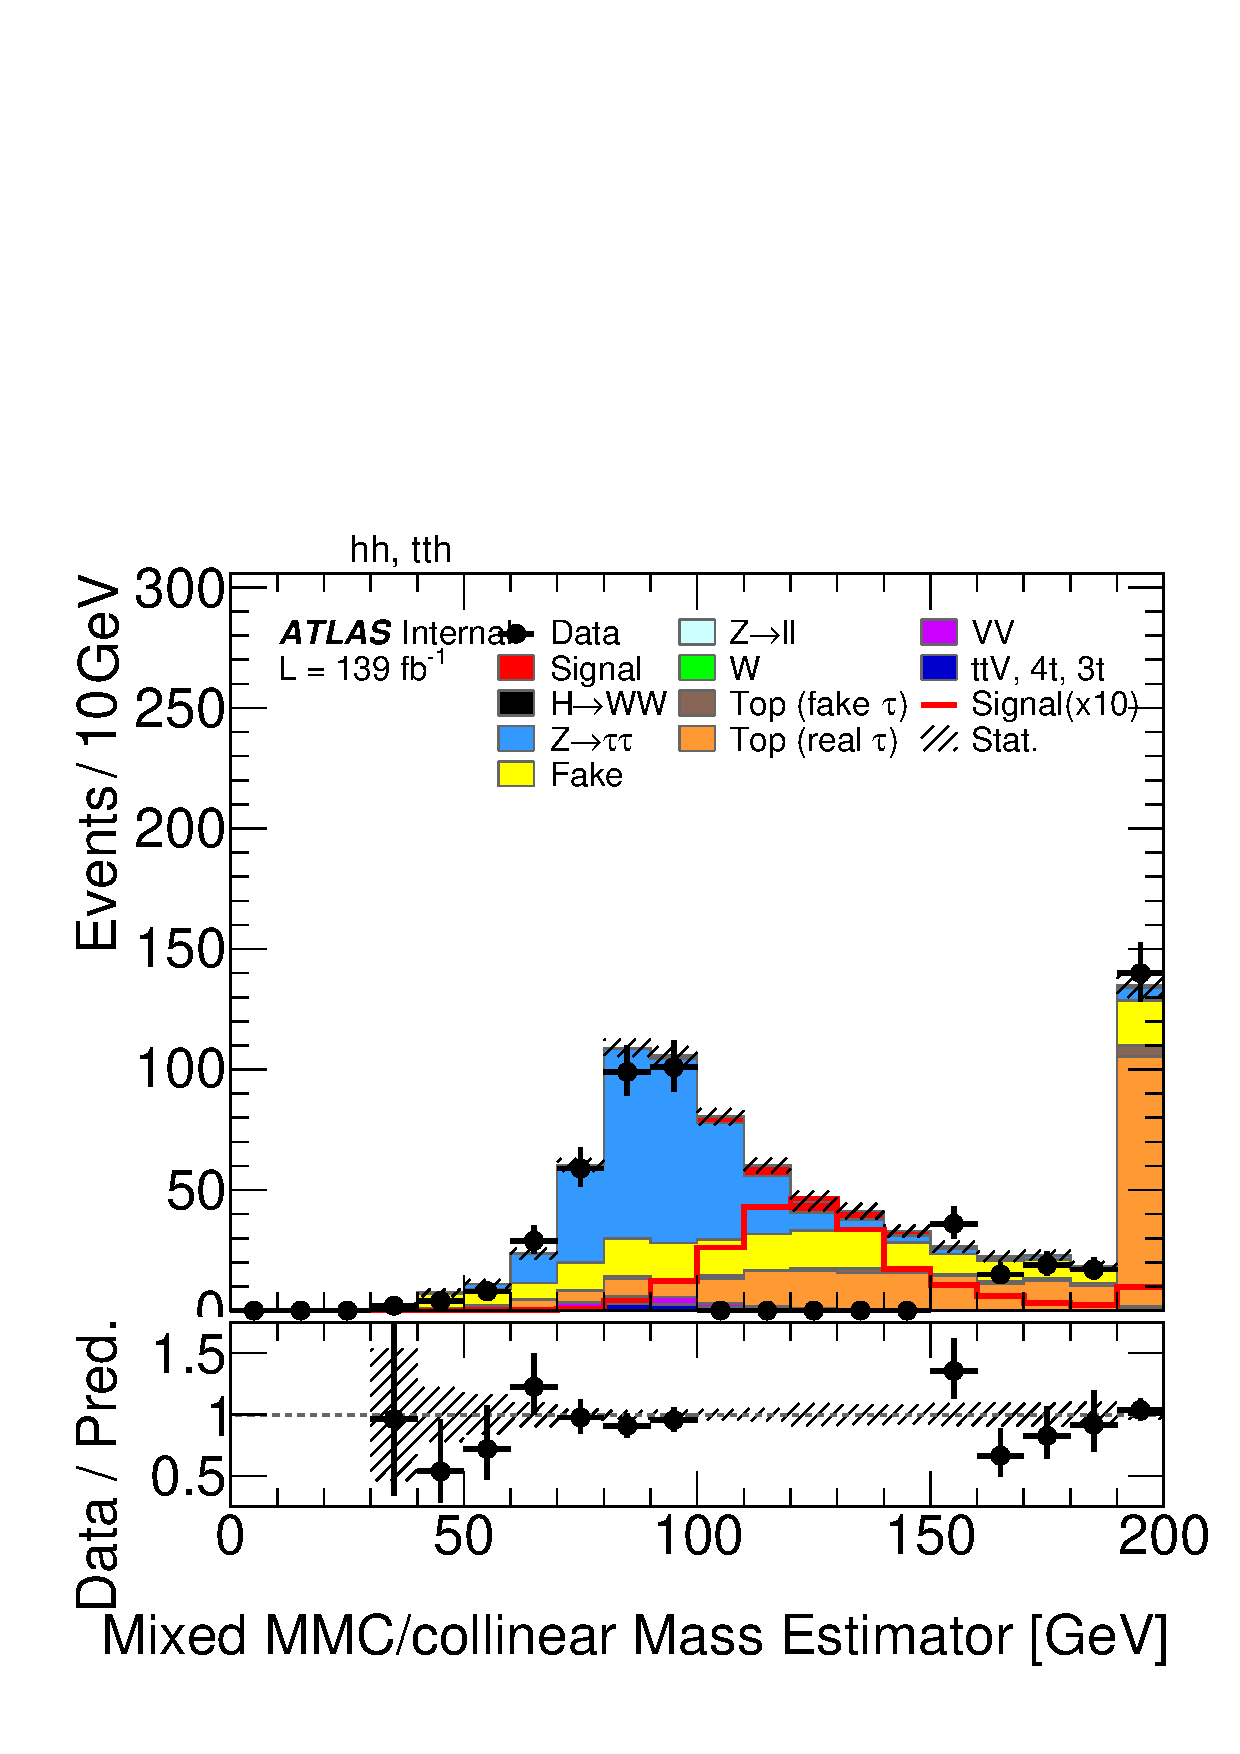
\includegraphics[width=\textwidth]{plot_ditau_mmc_mlm_m_fix_hh_tth.pdf}
      \caption{}
      \label{reconstructed_preselection_a}
  \end{subfigure}
  \hfill
  \begin{subfigure}[b]{0.48\textwidth}
      \centering
      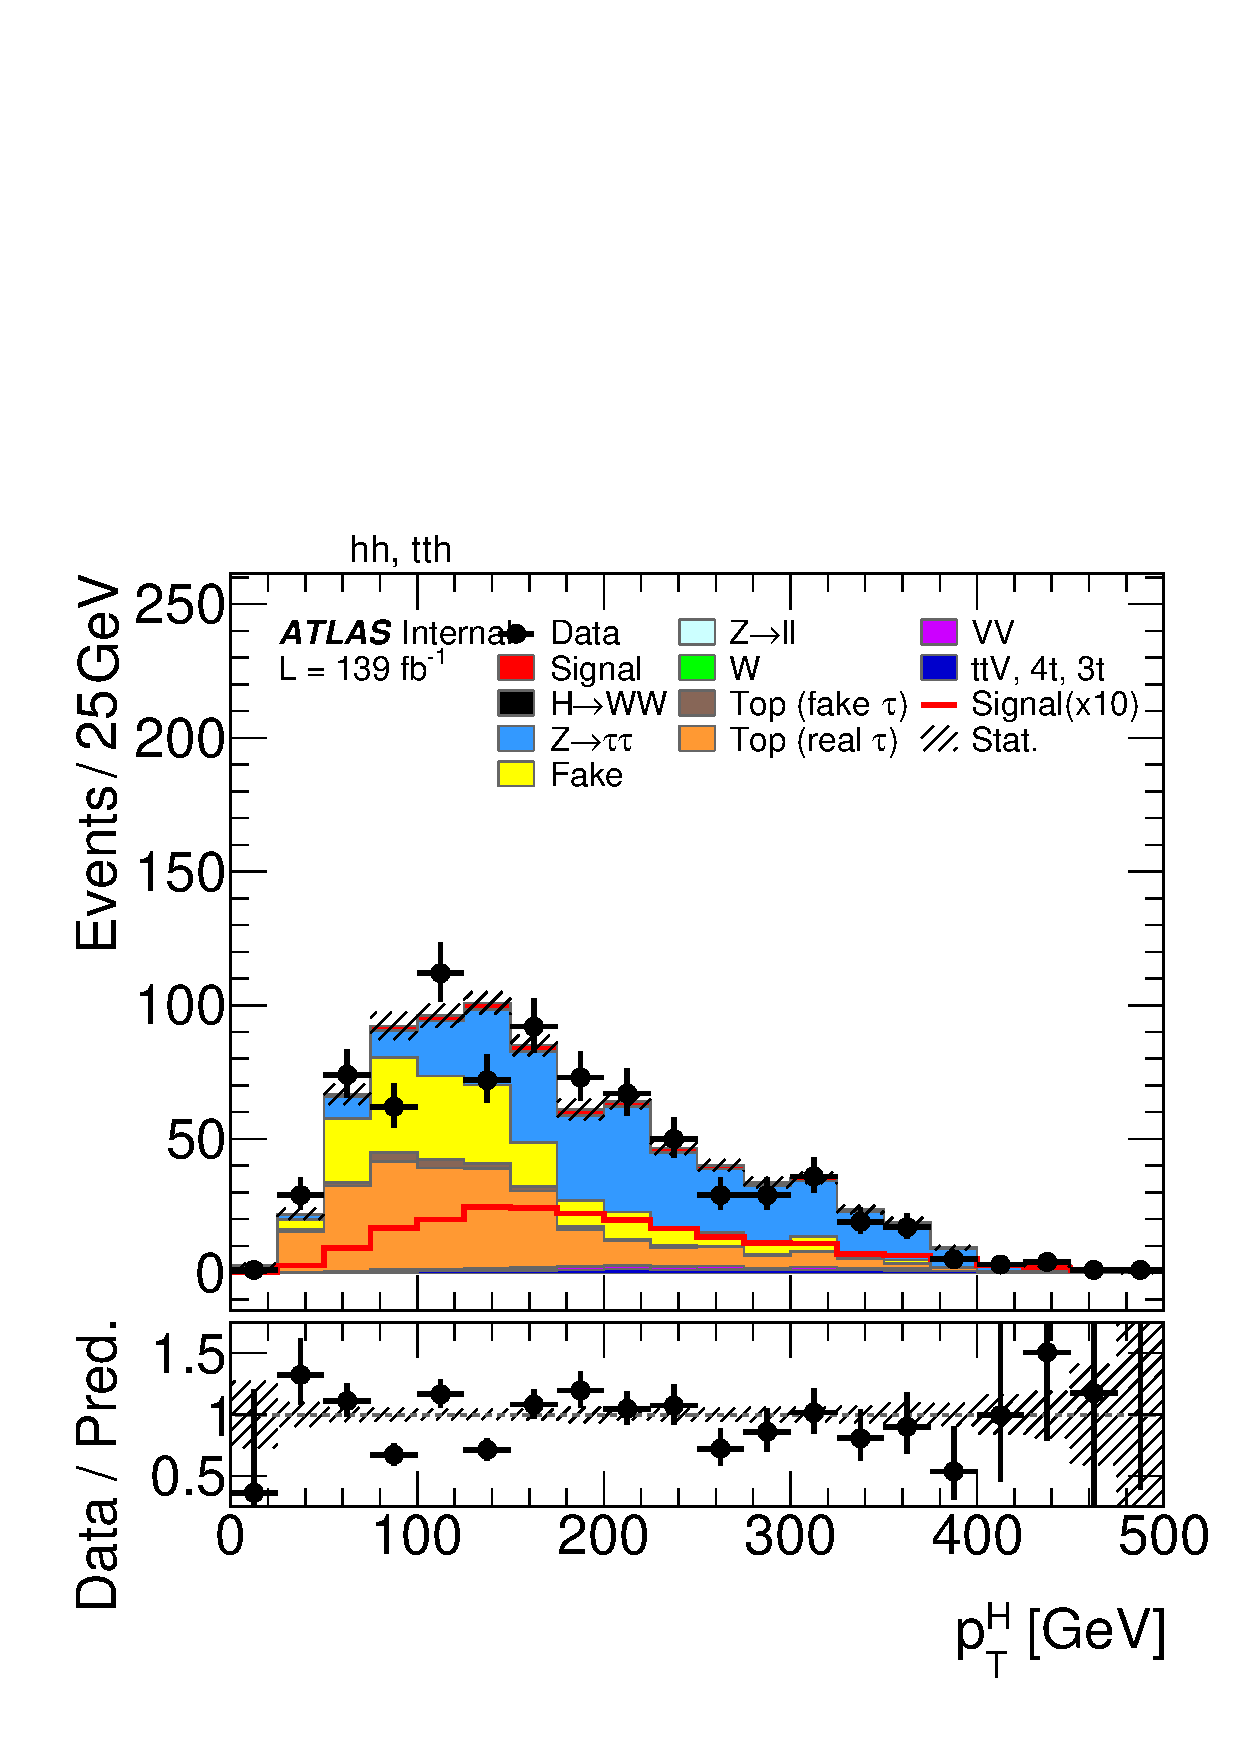
\includegraphics[width=\textwidth]{plot_ditau_pt_NN_kin_hh_tth.pdf}
      \caption{}
      \label{reconstructed_preselection_b}
  \end{subfigure}
  \caption{Distribuciones de (a) la \mmc con el rango $100-150$~GeV \textit{blinded}, y (b) $p_{\text{T}}^H$, mostradas al nivel de preselección de $t\bar{t}H$. Solo se incluyen las incertidumbres estadísticas.}
  \label{reconstructed_preselection}
\end{figure}

En lo que respecta a la separación de señal y fondo, esta se lleva a cabo mediante un discriminante multivariante (MVA) entrenado con \textsc{tmva} de \textsc{root}~\cite{tmvatoolkit}, empleando un BDT multicategoría. Se entrena conjuntamente para las tres clases que tenemos, con la señal \(\ttH\) frente a los principales fondos ($\ttbar$+jets y $Z\to\tau\tau$). Las variables de entrada incluyen cinemática de los taus, jets y $b$-jets, variables angulares y reconstrucciones parciales de masas invariantes. La respuesta del discriminante proporciona una separación potente, que ha sido mejorada respecto 
de la ronda anterior de este análisis donde se usaban dos BDTs binomiales para cada fondo. Además, se realizan entrenamientos dedicados para \pth$< 200$~GeV y \pth$> 200$~GeV, dado que en cada región varía la contribución de nuestro fondo y así ganaremos sensibilidad sobre los distintos STXS bins que medimos en el ajuste estadístico final.

\begin{figure}[htbp]
  \centering
  \setlength{\tabcolsep}{1.5pt}
  \renewcommand{\arraystretch}{0}
  \begin{tabular}{@{}c c c@{}}
    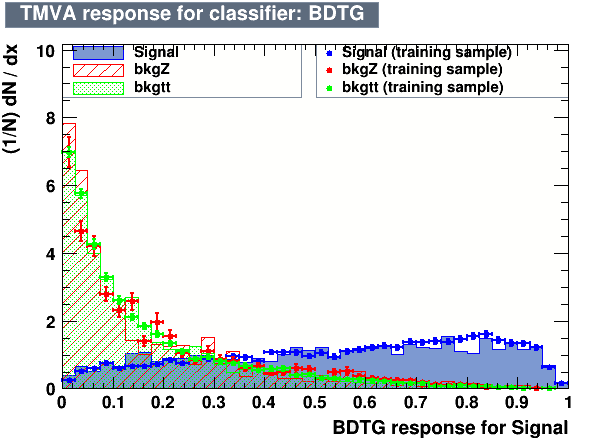
\includegraphics[width=0.33\textwidth]{images/plots_overtrain_lt200/overtrain_Signal_BDTG.png} &
    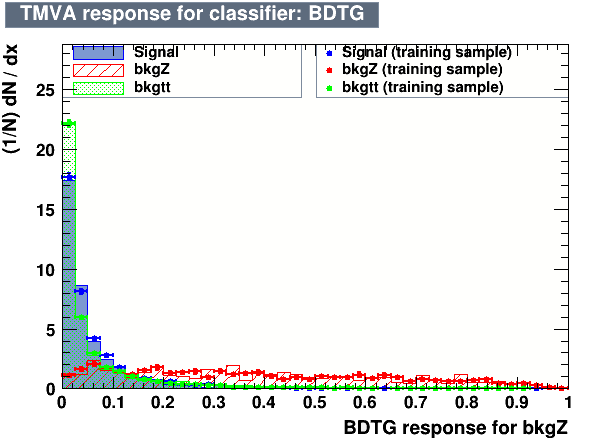
\includegraphics[width=0.33\textwidth]{images/plots_overtrain_lt200/overtrain_bkgZ_BDTG.png} &  
    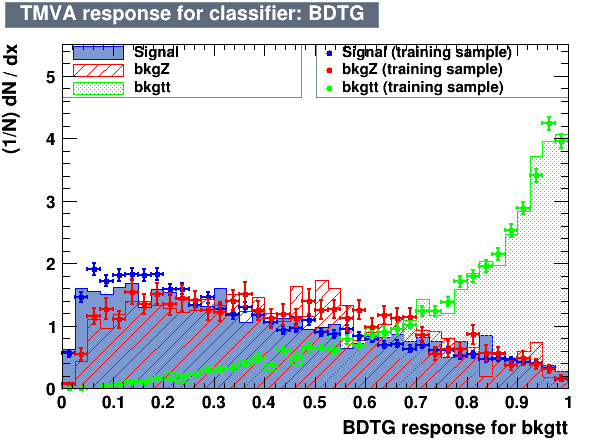
\includegraphics[width=0.33\textwidth]{images/plots_overtrain_lt200/overtrain_bkgtt_BDTG.png}
  \end{tabular}
  \caption{Distribuciones de los tres discriminantes del BDT entrenado a bajo \pth.}
  \label{lowpt_scores}
\end{figure}

\begin{figure}[htbp]
  \centering
  \setlength{\tabcolsep}{1.5pt}
  \renewcommand{\arraystretch}{0}
  \begin{tabular}{@{}c c c@{}}
    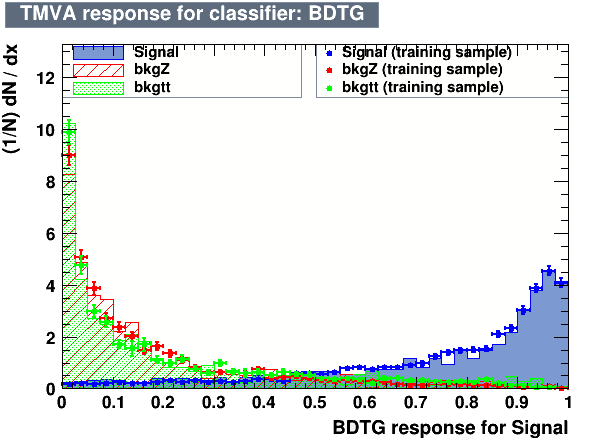
\includegraphics[width=0.33\textwidth]{images/plots_overtrain_gt200/overtrain_Signal_BDTG.png} &
    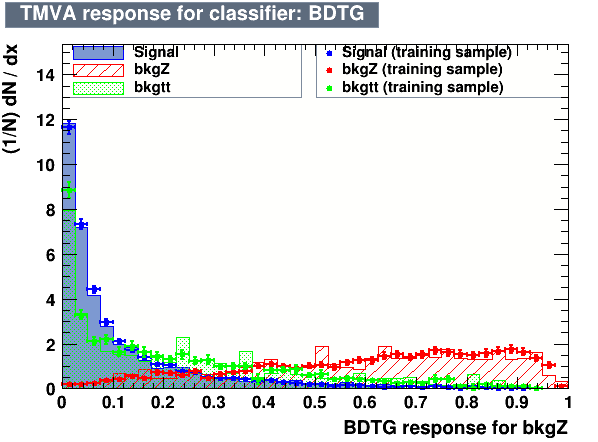
\includegraphics[width=0.33\textwidth]{images/plots_overtrain_gt200/overtrain_bkgZ_BDTG.png} &  
    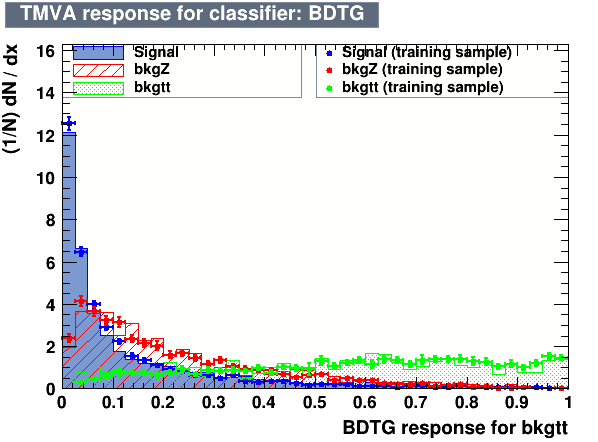
\includegraphics[width=0.33\textwidth]{images/plots_overtrain_gt200/overtrain_bkgtt_BDTG.png}
  \end{tabular}
  \caption{Distribuciones de los tres discriminantes del BDT entrenado a alto \pth.}
  \label{highpt_scores}
\end{figure}

Para la definición de las regiones de este ajuste, se construyen regiones de señal (SR) centradas en altos valores del discriminante BDT, y regiones de control (CR) para normalizar los fondos dominantes: una CR para $\ttbar$ y otra para $Z\to\tau\tau$, combinando cortes en los tres discriminantes que nos proporciona el BDT, en ambas regiones de \pth. Esta estrategia asegura un control directo de las normalizaciones de los principales fondos a partir de los datos. En el ajuste final, los factores de normalización (NFs) de $\ttbar$ y $Z\to\tau\tau$ se dejan libres, lo que permite que las distribuciones se ajusten dinámicamente a los datos.

Finalmente en el análisis estadístico, se realizan tres ajustes, teniendo como objetivo medir la \textit{signal strength} de la producción combinada de \htautau, de la producción a través de cada uno de los modos de producción (ggF, VBF, $VH$ y \ttH), y finalmente la medida diferencial en cada uno de los diferentes STXS bins, siendo un total de tres para \tth en \pth: por debajo de 120~GeV, entre 200 y 300~GeV, y por encima de 300~GeV.
De la medida inclusiva del modo de producción de \ttH en \htautau se obtiene como resultado:
\[
  \mu_{\ttH}^{\tau\tau} = 0.77 \pm 0.97,
\]
compatible con la predicción del Modelo Estándar. Este resultado mejora en torno a un 18\% la precisión relativa respecto a la iteración previa del análisis, en la que se obtuvo \(\mu_{\ttH}^{\tau\tau}=1.06^{+1.28}_{-1.08}\).

En lo que respecta al ajuste de STXS bins, se consiguieron las siguientes medidas para la \textit{signal strength} y la correspondiente sección eficaz:
\begin{itemize}
  \small
  \item $p_{\text{T}}^{H} < 200$~GeV:  
  \[
  \sigma \times B(H \to \tau\tau)=0.056^{+0.046}_{-0.044} 
  = 0.056^{+0.023}_{-0.019}(\text{syst.})\pm 0.035(\text{stat.})\text{pb}
  \]
  \[
  \mu \;=\; 2.2^{+1.8}_{-1.5}=2.2^{+0.84}_{-0.75}(\text{syst.})\pm 1.5(\text{stat.})
  \]
  \item $200 \leq p_{\text{T}}^{H} < 300$~GeV:  
  \[
  \sigma \times B(H \to \tau\tau) \;=\; -0.009^{+0.005}_{-0.005} 
  = -0.009^{+0.003}_{-0.004}(\text{syst.})\pm 0.003(\text{stat.}) \text{pb}
  \]
  \[
  \mu=-2.2^{+1.3}_{-1.1}=-2.2^{+0.58}_{-0.68}(\text{syst.})\pm 1.1(\text{stat.})
  \]
  \item $p_{\text{T}}^{H} \geq 300$~GeV:  
  \[
  \sigma \times B(H \to \tau\tau) \;=\; 0.029^{+0.023}_{-0.018} 
  = 0.029^{+0.009}_{-0.008}(\text{syst.})^{+0.021}_{-0.017}(\text{stat.})\text{pb}
  \]
  \[
  \mu=3.6^{+2.9}_{-2.3}=3.6^{+1.3}_{-0.9}(\text{syst.})^{+2.6}_{-2.1}(\text{stat.})
  \]
\end{itemize}

El ajuste de los principales procesos de fondo se controla mediante factores de normalización libres, que resultan en
\[
  \text{NF}(\ttbar) = 1.08 \pm 0.12, \qquad \text{NF}(Z\to\tau\tau) = 0.95 \pm 0.15.
\]
Estos valores muestran la coherencia del modelado de los fondos tras ser ajustados con datos en las regiones de control.

Las incertidumbres sistemáticas dominantes en estas medidas corresponden al modelado teórico de \(\ttbar\) y la señal de \ttH, a la calibración de taus y jets, y a la escala de energía de los jets (JES). En conjunto, las sistemáticas contribuyen de forma comparable al componente estadístico de la incertidumbre total, reflejando que el análisis se encuentra todavía limitado por la estadística disponible. 

Los resultados obtenidos para los tres bins de \pth sufren de baja precisión, dado el reducido tamaño de la muestra. Por ello, para estos tres parámetros se calculan también sus límites superiores, que constituyen las primeras restricciones de ATLAS para \(\ttH(\tau\tau)\) en esta segmentación del espacio de fases.

\begin{figure}[h]
  \centering
  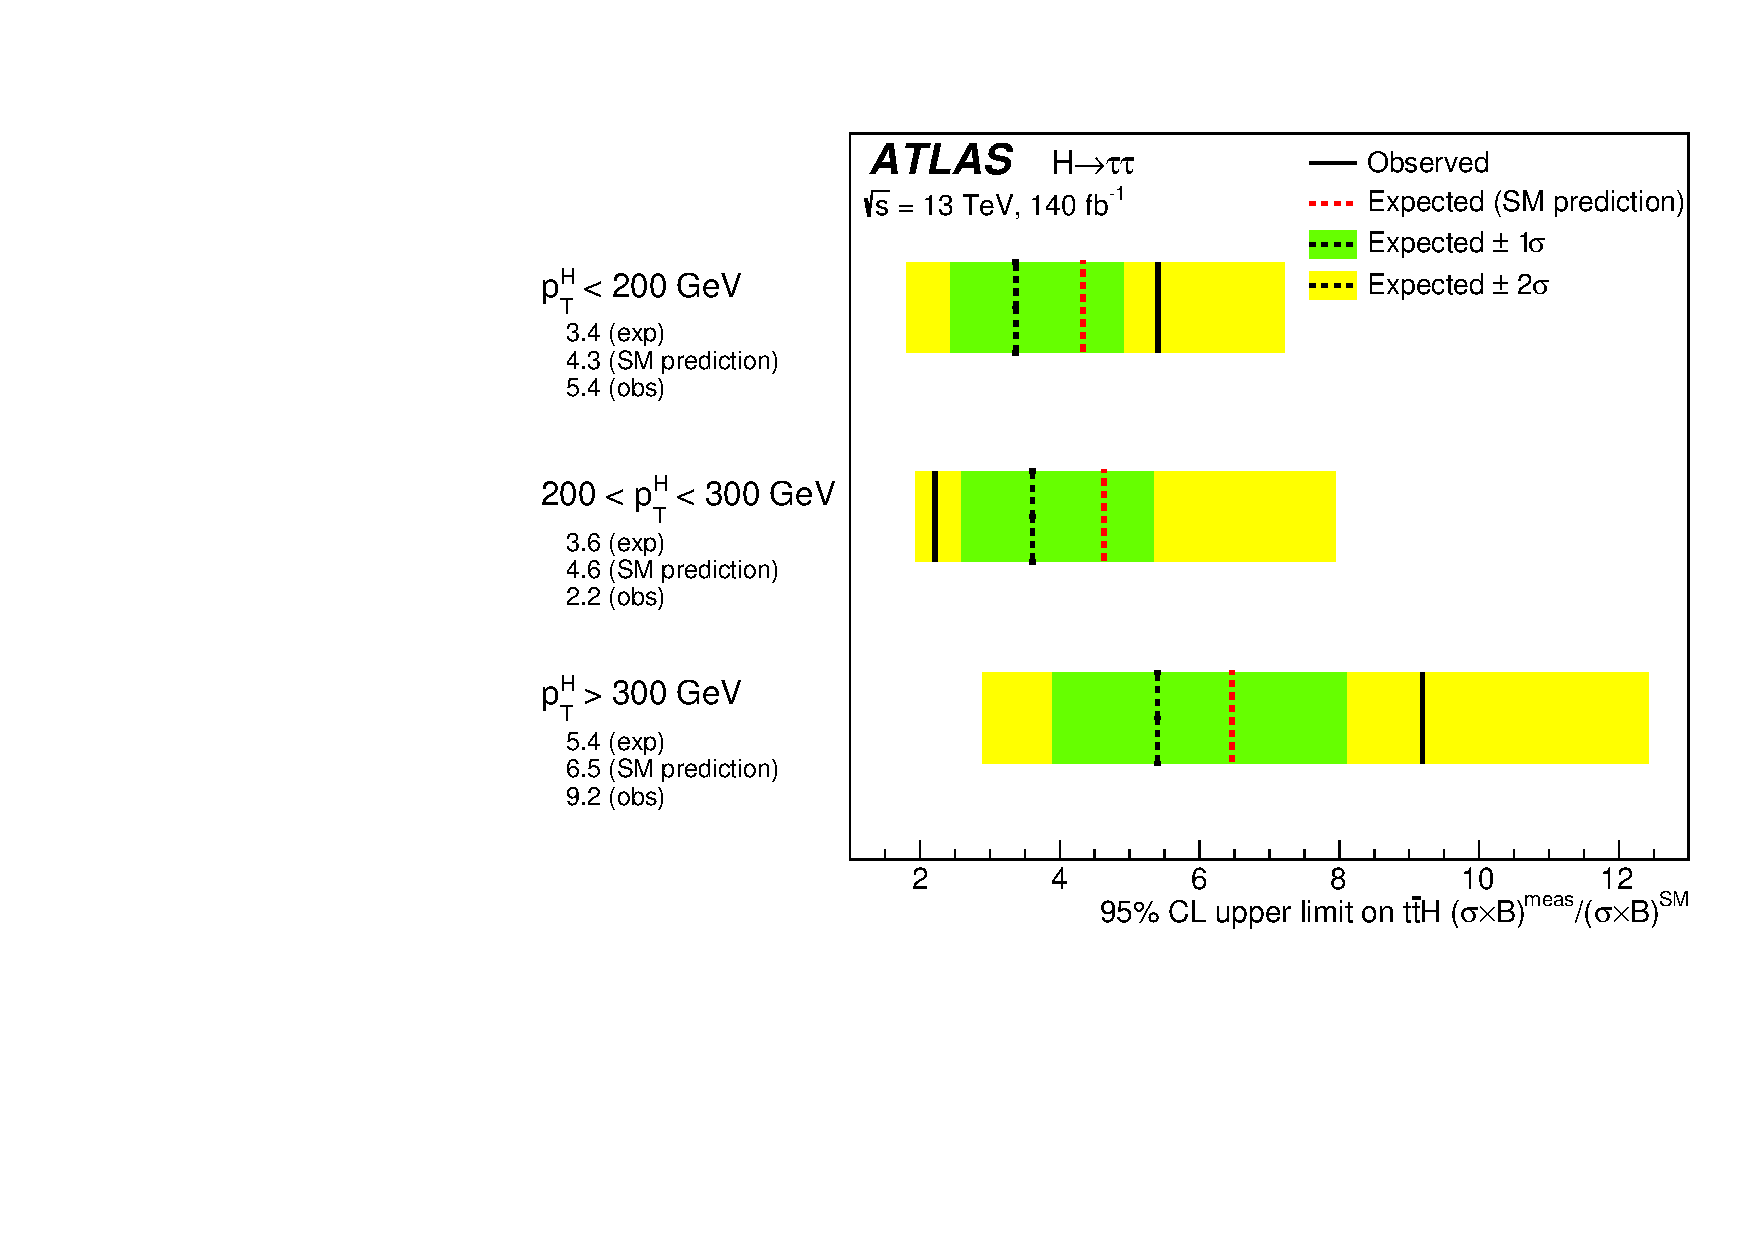
\includegraphics[width=0.70\linewidth]{images/fit_stxs/fig_08.pdf} % <-- sustituye ruta/nombre
  \caption{Límites superiores al 95\% CL sobre las medidas de STXS de \ttH\ en los distintos intervalos de $p_{\mathrm{T}}^{H}$, mostrados de forma relativa a la predicción del SM y derivados mediante el método $CL_s$. Los límites observados se indican con líneas negras continuas, mientras que los límites esperados bajo la hipótesis de sólo fondo (SM) se muestran con líneas negras (rojas) discontinuas. Para el caso de sólo fondo, se representan también las bandas de incertidumbre correspondientes a $\pm 1\sigma$ y $\pm 2\sigma$.}
  \label{res:tth_cls_limits}
\end{figure}

En conclusión, el análisis \(\ttH(\tau_{\mathrm{had}}\tau_{\mathrm{had}})\) en ATLAS con la muestra completa de Run-2 constituye un avance significativo en la exploración de este proceso. A pesar de la dificultad experimental inherente al canal, se han obtenido resultados consistentes con el Modelo Estándar, se han reducido las incertidumbres respecto a estudios previos y se ha demostrado la viabilidad de extender la medida a categorías diferenciales en el marco STXS. La metodología desarrollada, en particular la categorización optimizada y el uso de un discriminante BDT multiclase, sienta las bases para análisis más precisos al incluir datos de Run~3, donde la estadística adicional puede reducir de forma notable las incertidumbres y mejorar las restricciones sobre el acoplamiento de Yukawa del top.

\FloatBarrier


%%%%%%%%%%%%%%%%%%%%%%%%%%%%%%%%%%%%%%%%%%%%%%%%%%%%%%%%%%%%%%%%%%%%%%%%%%%%%%%%%%%%%%%%%%%%%%%%%%%%%%%%%%%%%%%%%%%%%%%%%%%%%%%%%%%%%%%%%%%%%%%%%%%%%%%%%%
\section*{Medida de \thqb + \ttH con \htautau con datos de Run-2 y parte de Run-3}
%%%%%%%%%%%%%%%%%%%%%%%%%%%%%%%%%%%%%%%%%%%%%%%%%%%%%%%%%%%%%%%%%%%%%%%%%%%%%%%%%%%%%%%%%%%%%%%%%%%%%%%%%%%%%%%%%%%%%%%%%%%%%%%%%%%%%%%%%%%%%%%%%%%%%%%%%%

La producción asociada de un bosón de Higgs con quarks top, en sus modos \ttH y \thqb, constituye una oportunidad única para estudiar la estructura de $CP$ del acoplamiento de Yukawa del top. En el Modelo Estándar el Higgs es un escalar puro y sus interacciones son $CP$-par ($CP$-even), pero escenarios con mezcla escalar–pseudoscalar siguen siendo compatibles con los datos actuales y aportarían nuevas fuentes de violación de $CP$ de interés cosmológico~\cite{Gunion:1996xu, Ellis:2013yxa, He:2015spx, Boudjema:2015nda}. 
La interacción Higgs–top se puede escribir como una modificación del término de Yukawa con un ángulo de mezcla $\alpha$ que interpola entre los límites puramente escalar y puramente pseudoscalar, como se muestra en la Figura~\ref{res:th_cp_dependence}; en este contexto, tanto la sección eficaz inclusiva de \ttH como, especialmente, la de \tH\ dependen de $\alpha$. Una medida conjunta de \ttH\ y \thqb es, por tanto, particularmente sensible a posibles componentes CP-impares en el vértice $Ht\bar t$.

\begin{figure}[htbp]
  \centering
  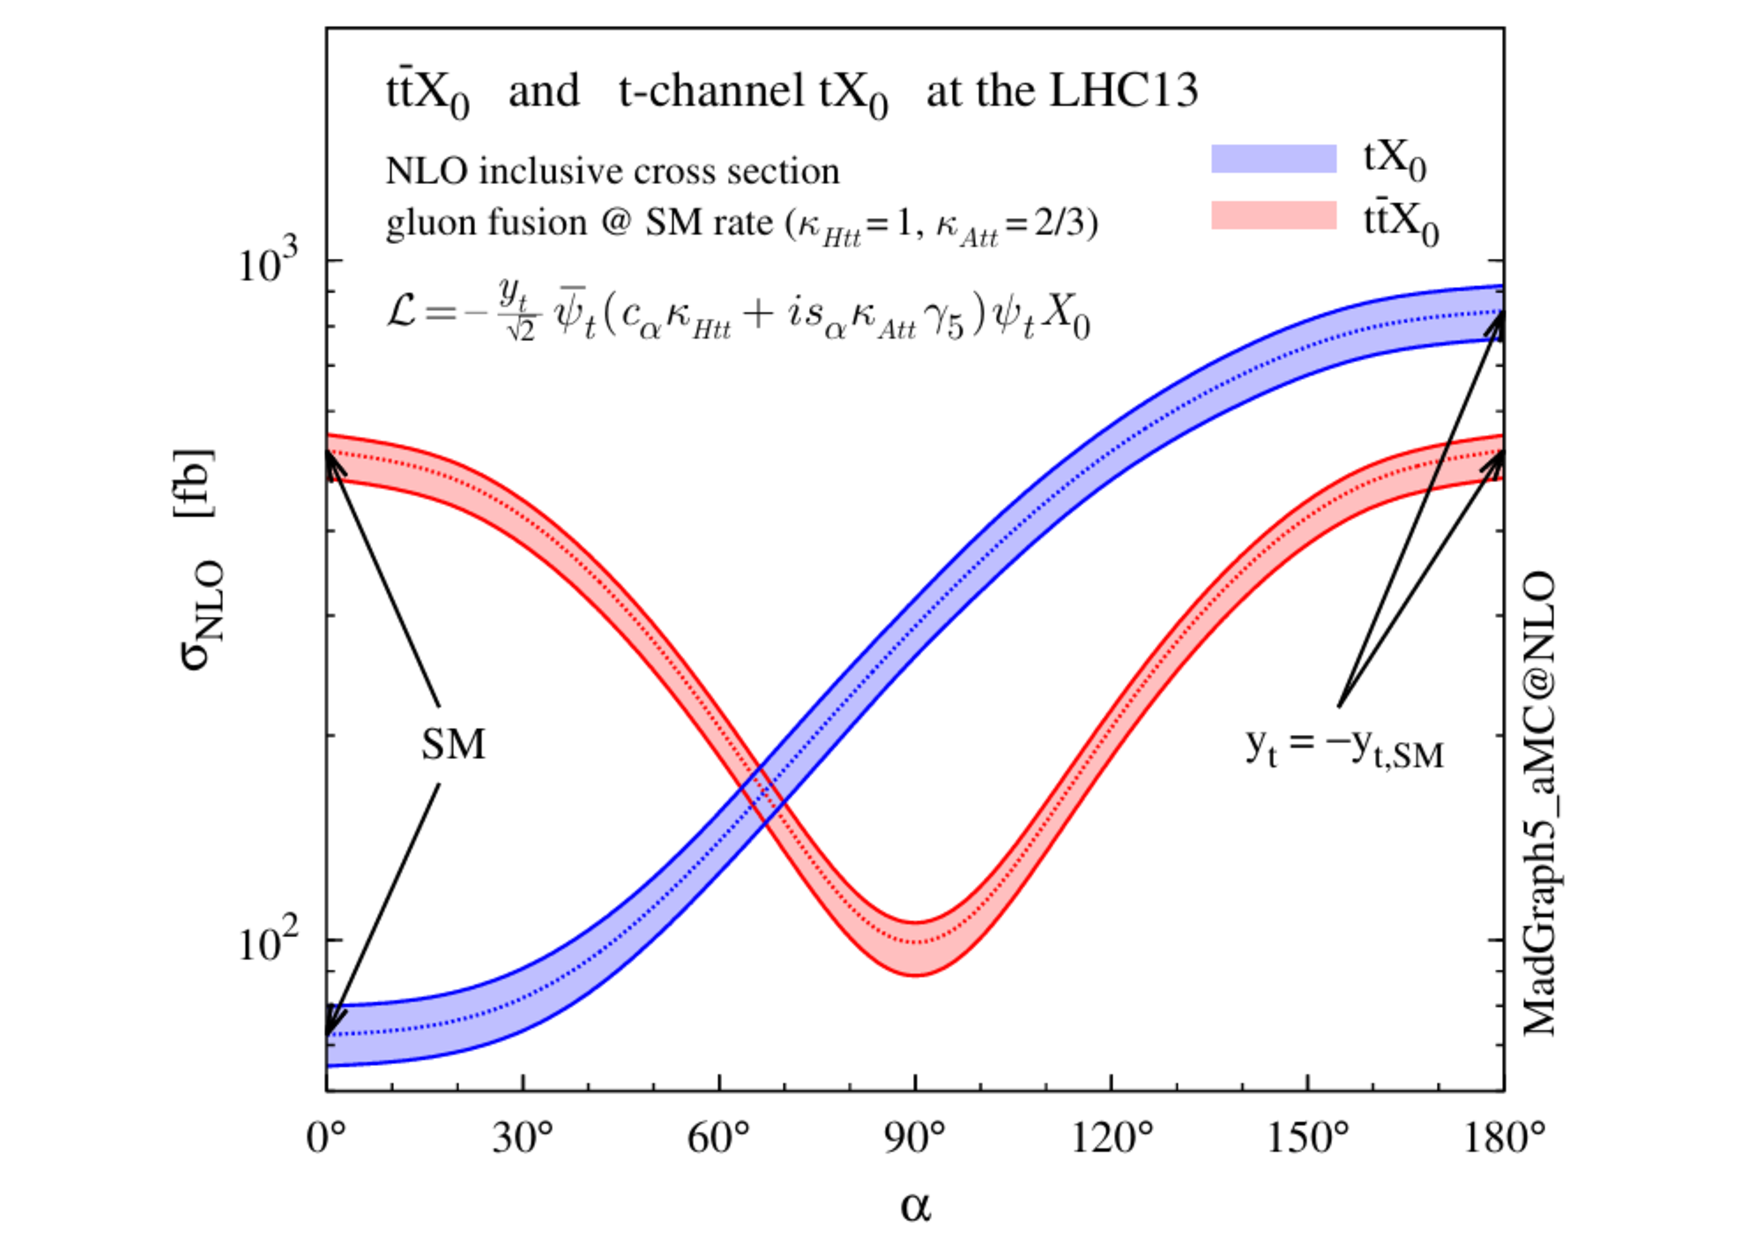
\includegraphics[width=0.65\textwidth]{cp_higgs.pdf}
  \caption{Secciones eficaces a NLO para la producción de $t\bar{t}H$ y $tH$ a $\sqrt{s}=13$~TeV en función del ángulo de mezcla $CP$ $\alpha$, incluyendo las incertidumbres de escala~\cite{demartin2015}.}
  \label{res:th_cp_dependence}
\end{figure}

En este capítulo se presenta un estudio combinado de \ttH y \thqb en \htautau en el canal completamente hadrónico, aprovechando la estadística de Run~2 junto con datos parciales de Run~3. El objetivo no es una combinación global de todos los modos de producción, sino cuantificar la sensibilidad alcanzable para \thqb en este canal, medido por primera vez en ATLAS, a la vez que se reevalúa \ttH con datos adicionales. En comparación con el análisis previo, la selección de eventos se ha modificado para adaptarse a la topología característica de \thqb, 
relajando los requisitos a un mínimo de cinco jets y al menos un b-jet, lo que permite aumentar la aceptación de señal sin perder el control del fondo dominante. Adicionalmente, se han implementado mejoras en la identificación de objetos: para la identificación de \tauhad se utiliza el nuevo algoritmo \textsc{gntau}, basado en grafos neuronales, que reduce significativamente la contribución de jets mal identificados como \tauhad, como se muestra en la Figura~\ref{res:fakes_new}; mientras que para el etiquetado de b-jets se emplea el modelo \textsc{gn2v01}~\cite{new_tagging}, un clasificador de tipo Transformer
que mejora la eficiencia de identificación respecto a la técnica usada en Run~2. Estas actualizaciones, junto con la estrategia MVA revisada, proporcionan un balance más favorable entre aceptación de señal y rechazo de fondo. Como en el análisis anterior, el fondo asociado a \tauhad erróneamente identificados se estima directamente a partir de datos, y se evalúan de nuevo las incertidumbres estadísticas asociadas a este procedimiento.
\begin{figure}[htbp]
  \centering
  % Top row: GNTau
  \begin{subfigure}[b]{0.45\textwidth}
      \centering
      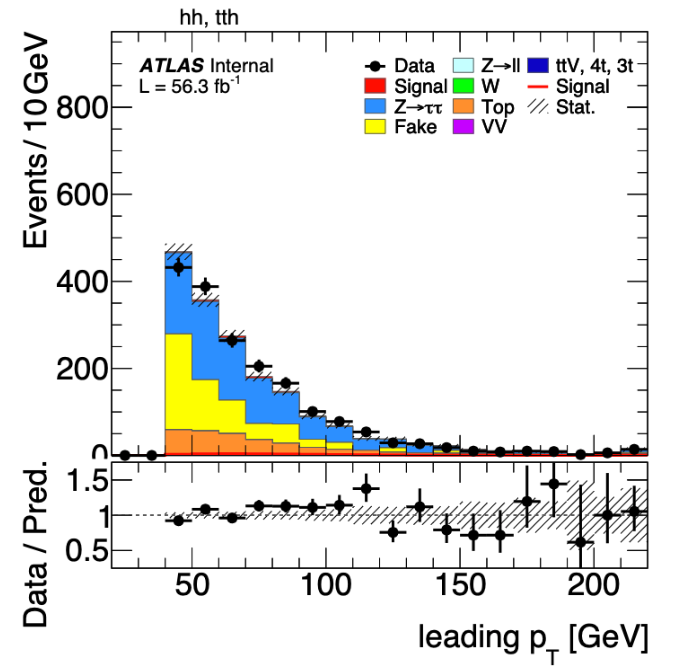
\includegraphics[width=\textwidth]{images/leading_pt_gntau.png}
      \caption{\textsc{gntau}}
  \end{subfigure}
  \begin{subfigure}[b]{0.45\textwidth}
      \centering
      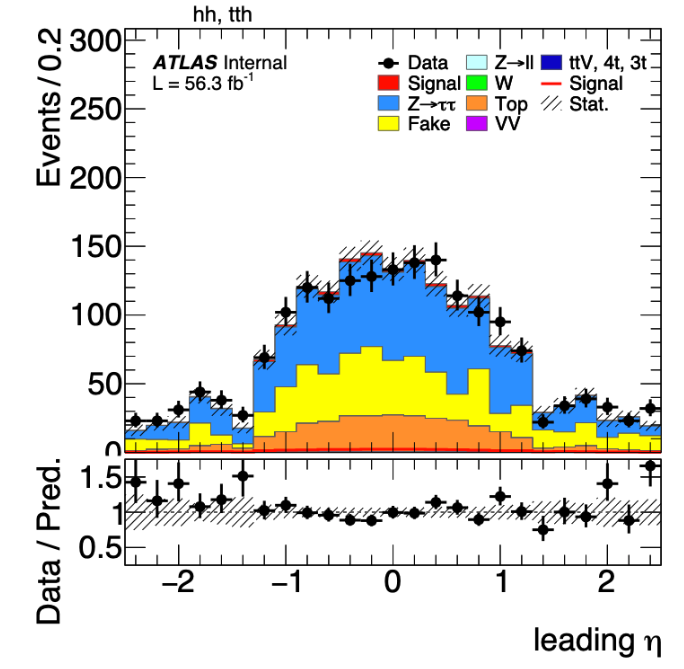
\includegraphics[width=\textwidth]{images/leading_eta_gntau.png}
      \caption{\textsc{gntau}}
  \end{subfigure}

  % Bottom row: RNN
  \begin{subfigure}[b]{0.45\textwidth}
      \centering
      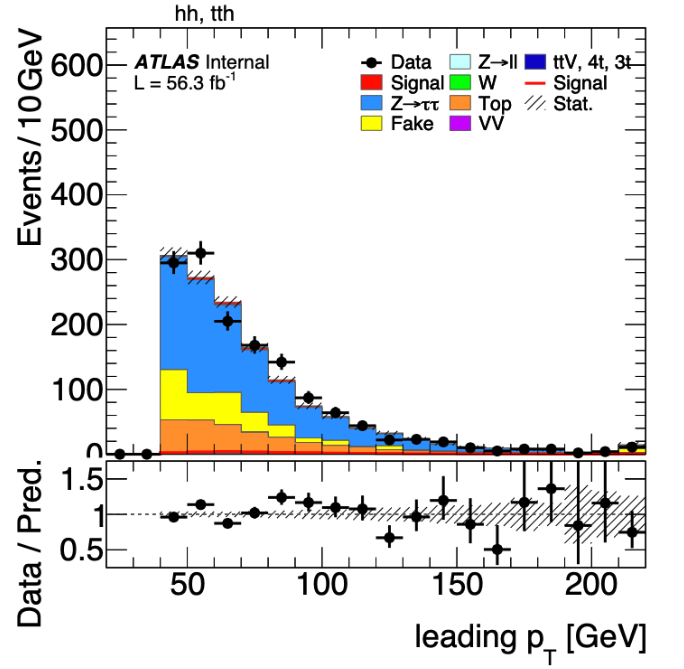
\includegraphics[width=\textwidth]{images/leading_pt_rnn.png}
      \caption{RNN-ID}
  \end{subfigure}
  \begin{subfigure}[b]{0.45\textwidth}
      \centering
      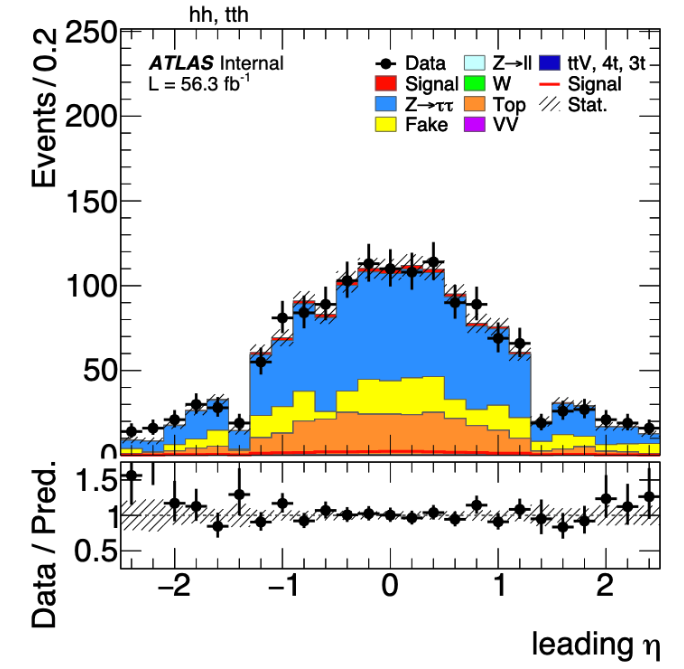
\includegraphics[width=\textwidth]{images/leading_eta_rnn.png}
      \caption{RNN-ID}
  \end{subfigure}

  \caption{Distribuciones del momento transverso y de la pseudorrapidez del candidato \tauhad principal en la preselección de \ttH con al menos un $b$-jet etiquetado. La fila superior muestra los resultados obtenidos con el nuevo algoritmo de identificación \textsc{gntau}, en (a) y (b), mientras que la fila inferior muestra las distribuciones correspondientes con el enfoque basado en RNN utilizado anteriormente, en (c) y (d). Estas distribuciones se evalúan en datos y simulaciones del periodo de toma de datos de 2022. Se aplican factores de escala sobre \ztautau y \ttbar. Solo se incluyen las incertidumbres estadísticas.
  }
  \label{res:fakes_new}
\end{figure}
El resto de fondos se estiman a partir de simulaciones MC, normalizando los fondos dominantes de $\ttbar$ y $Z\to\tau\tau$ a partir de los resultados del ajuste estadístico. 
En Run~3 se observan notables ineficiencias en el modelado de MC (especialmente en $Z\to\tau\tau$) que se abordan con factores de normalización libres en el ajuste. En las comparativas de Datos y MC, cuando procede, se emplean factores de escala ilustrativos (1.2 para $\ttbar$ y 1.4 para $Z\to\tau\tau$), consistentes con los valores que extraen finalmente el ajuste con datos en las CRs. 

En esta ronda, la clasificación se basa en un BDT multiclase con cuatro discriminantes como resultado, entrenado conjuntamente para \ttH, \thqb, $Z\to\tau\tau$ y $\ttbar$. Se reutilizan las variables ya empleadas para el BDT empleado en \ttH frente a fondos y se incorporan observables diseñados para maximizar la separación entre \ttH\ y \thqb, centrados en la cinemática y topología de \emph{light}-jets y $b$-jets: multiplicidades de \emph{light}-jets y $b$-jets, signo común de $\eta$ entre \emph{light}-jets, $\eta$ y $p_{\mathrm{T}}$ del $b$-jet principal, separaciones máximas en $\Delta\eta$ entre el Higgs y $b$-jets o entre \emph{light}- y $b$-jets, y la masa invariante máxima de dos \emph{light}-jets en el estado final. Estas variables capturan, por ejemplo, el carácter más \textit{forward} del \textit{light}-jet en \thqb y la diferente procedencia de los $b$-jets respecto a \ttH. Las distribuciones de algunas de ellas se muestran en la Figura~\ref{res:new_variables}
Además, el entrenamiento se realiza con las muestras MC combinadas de Run~2 y Run~3.

\begin{figure}[htbp]
  \centering
  % 1a fila
  \begin{subfigure}[b]{0.45\textwidth}
    \centering
    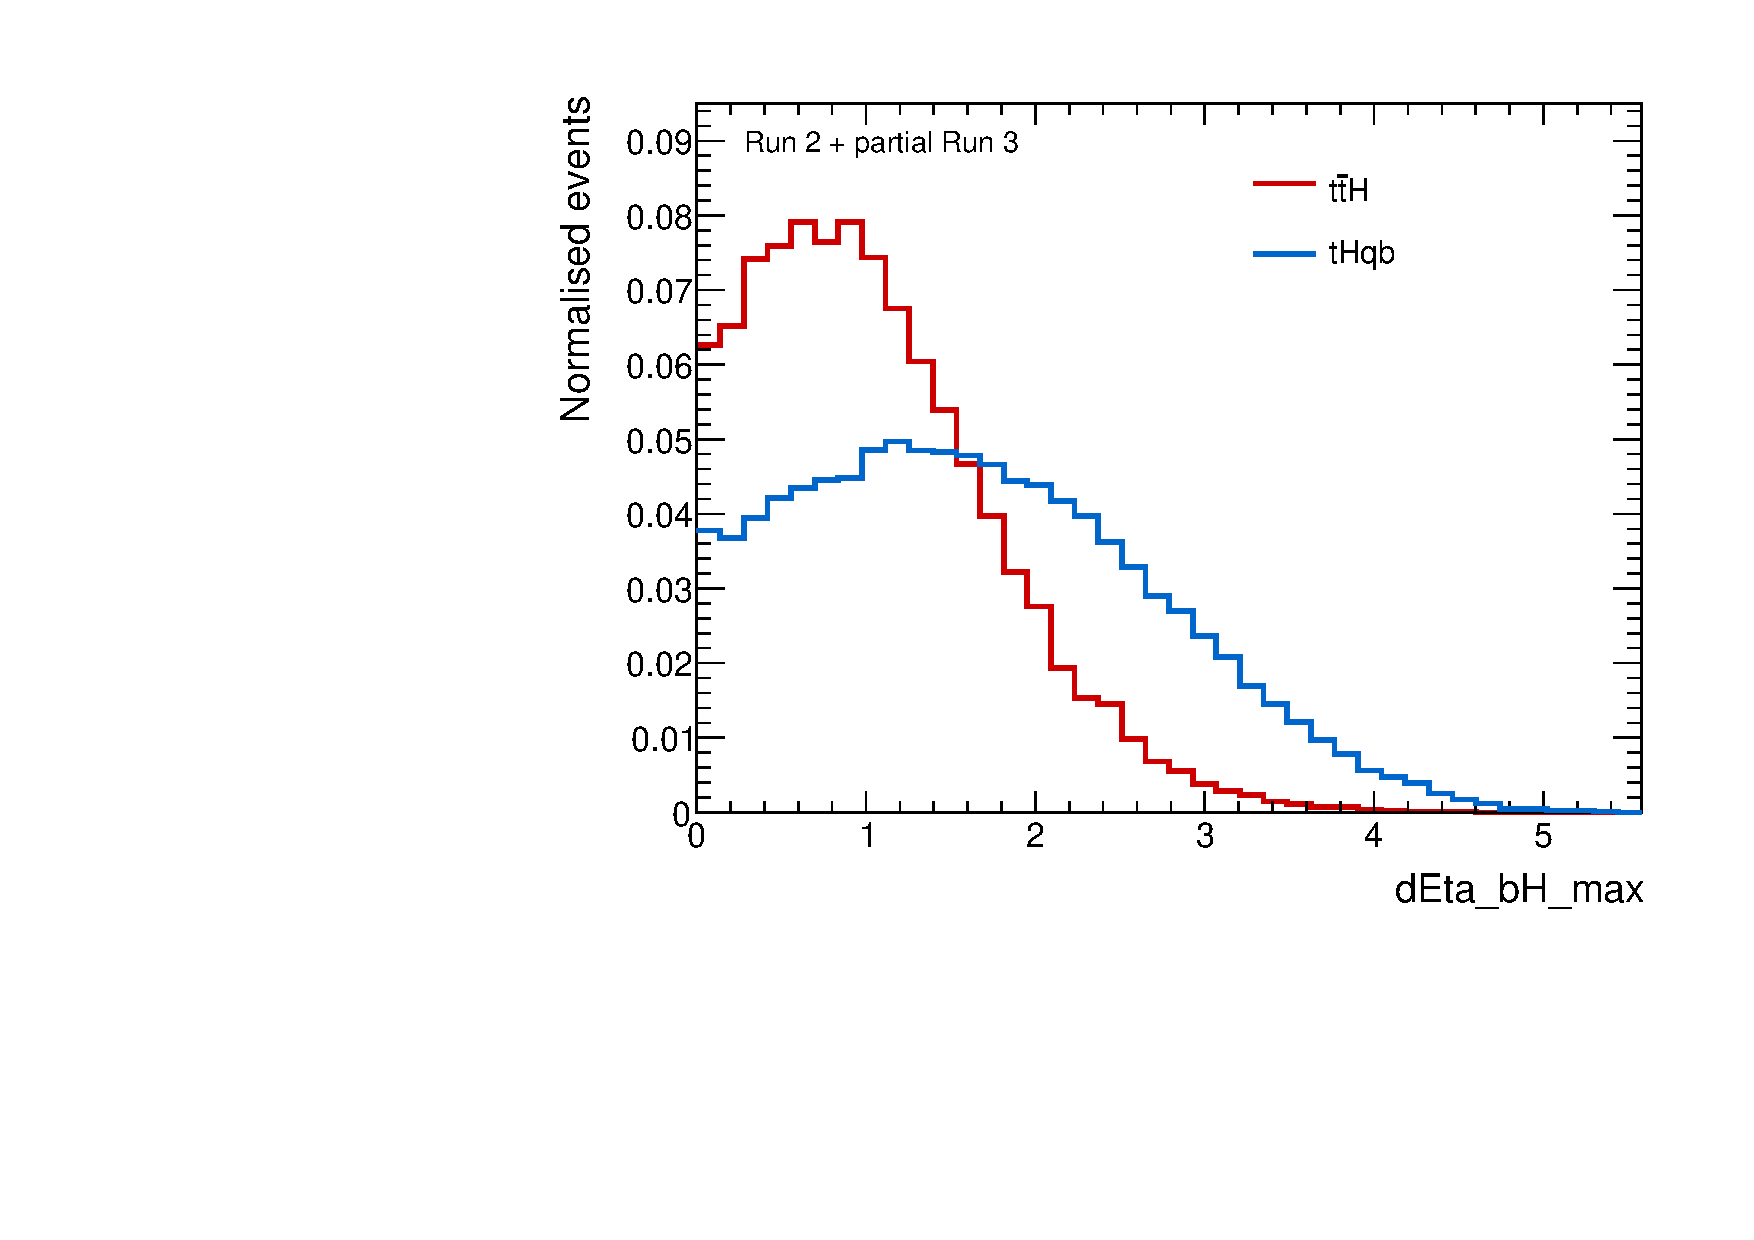
\includegraphics[width=\textwidth]{images/plots_tH_tHqb_for_thesis/dEta_bH_max_signals_ATLAS.pdf}
    \caption{Max.\ $\Delta \eta (H,b\text{jet})$}
    \label{fig:dEta_bH_max}
  \end{subfigure}
  \hfill
  \begin{subfigure}[b]{0.45\textwidth}
    \centering
    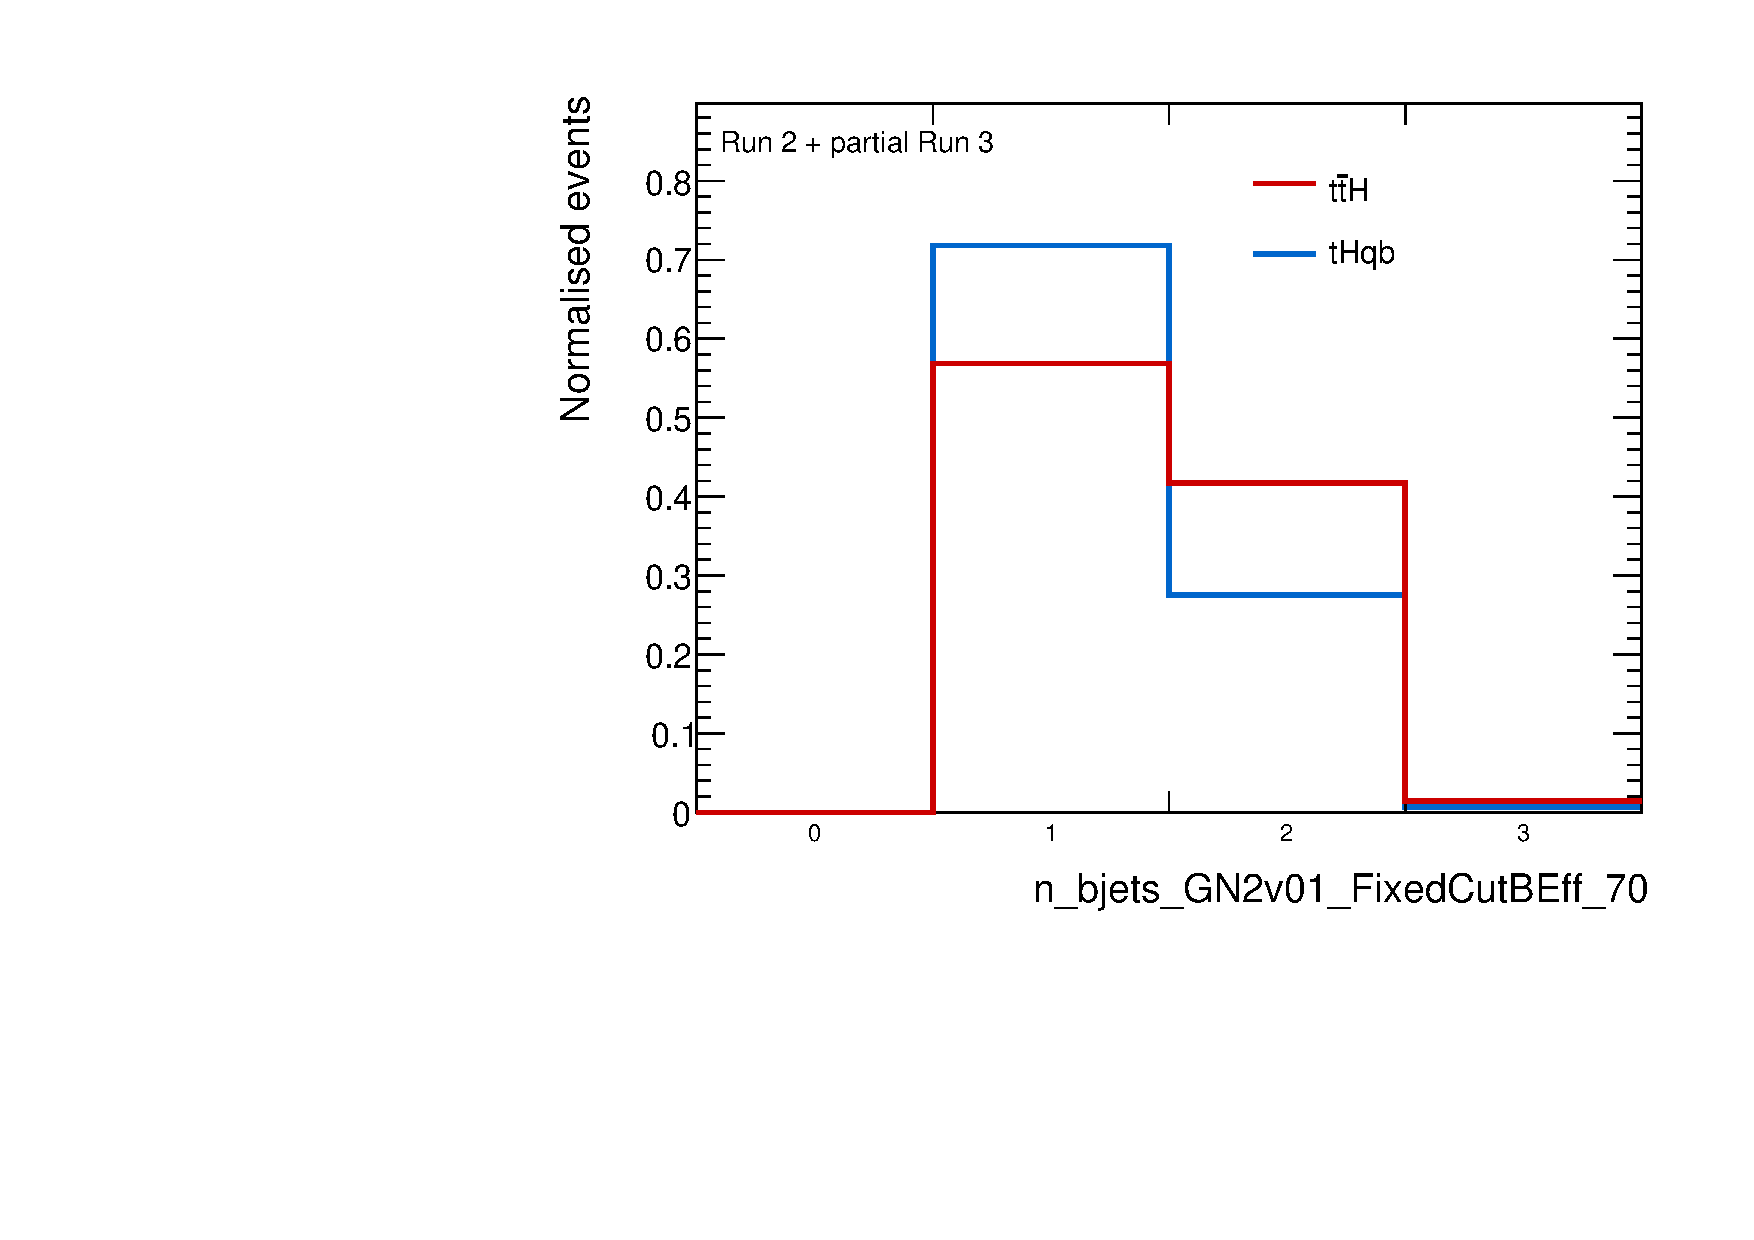
\includegraphics[width=\textwidth]{images/plots_tH_tHqb_for_thesis/n_bjets_GN2v01_FixedCutBEff_70_signals_ATLAS.pdf}
    \caption{$b$-jet multiplicity}
    \label{fig:n_bjets}
  \end{subfigure}

  % 2a fila
  \vskip\baselineskip
  \begin{subfigure}[b]{0.45\textwidth}
    \centering
    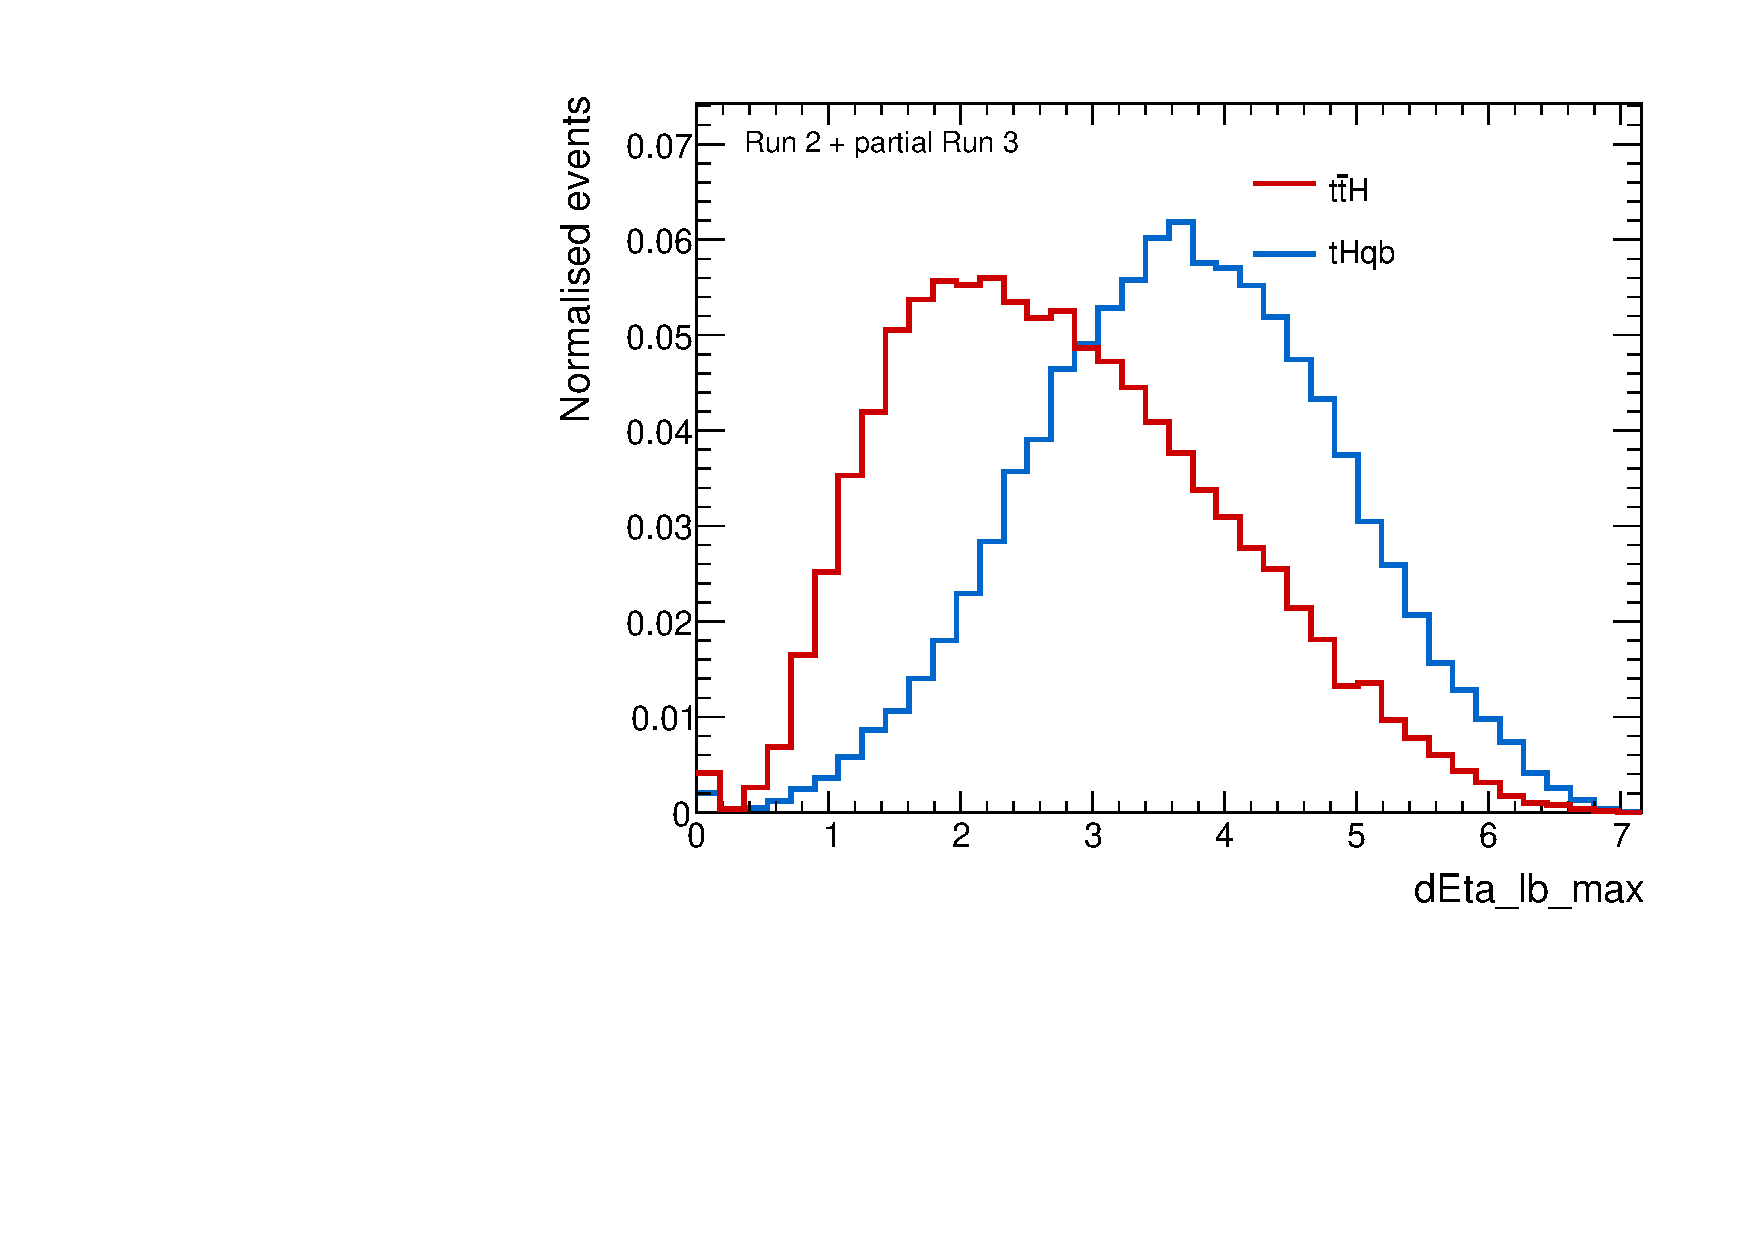
\includegraphics[width=\textwidth]{images/plots_tH_tHqb_for_thesis/dEta_lb_max_signals_ATLAS.pdf}
    \caption{Max.\ $\Delta \eta (l\text{jet},b-\text{jet})$}
    \label{fig:dEta_lb_max}
  \end{subfigure}
  \hfill
  \begin{subfigure}[b]{0.45\textwidth}
    \centering
    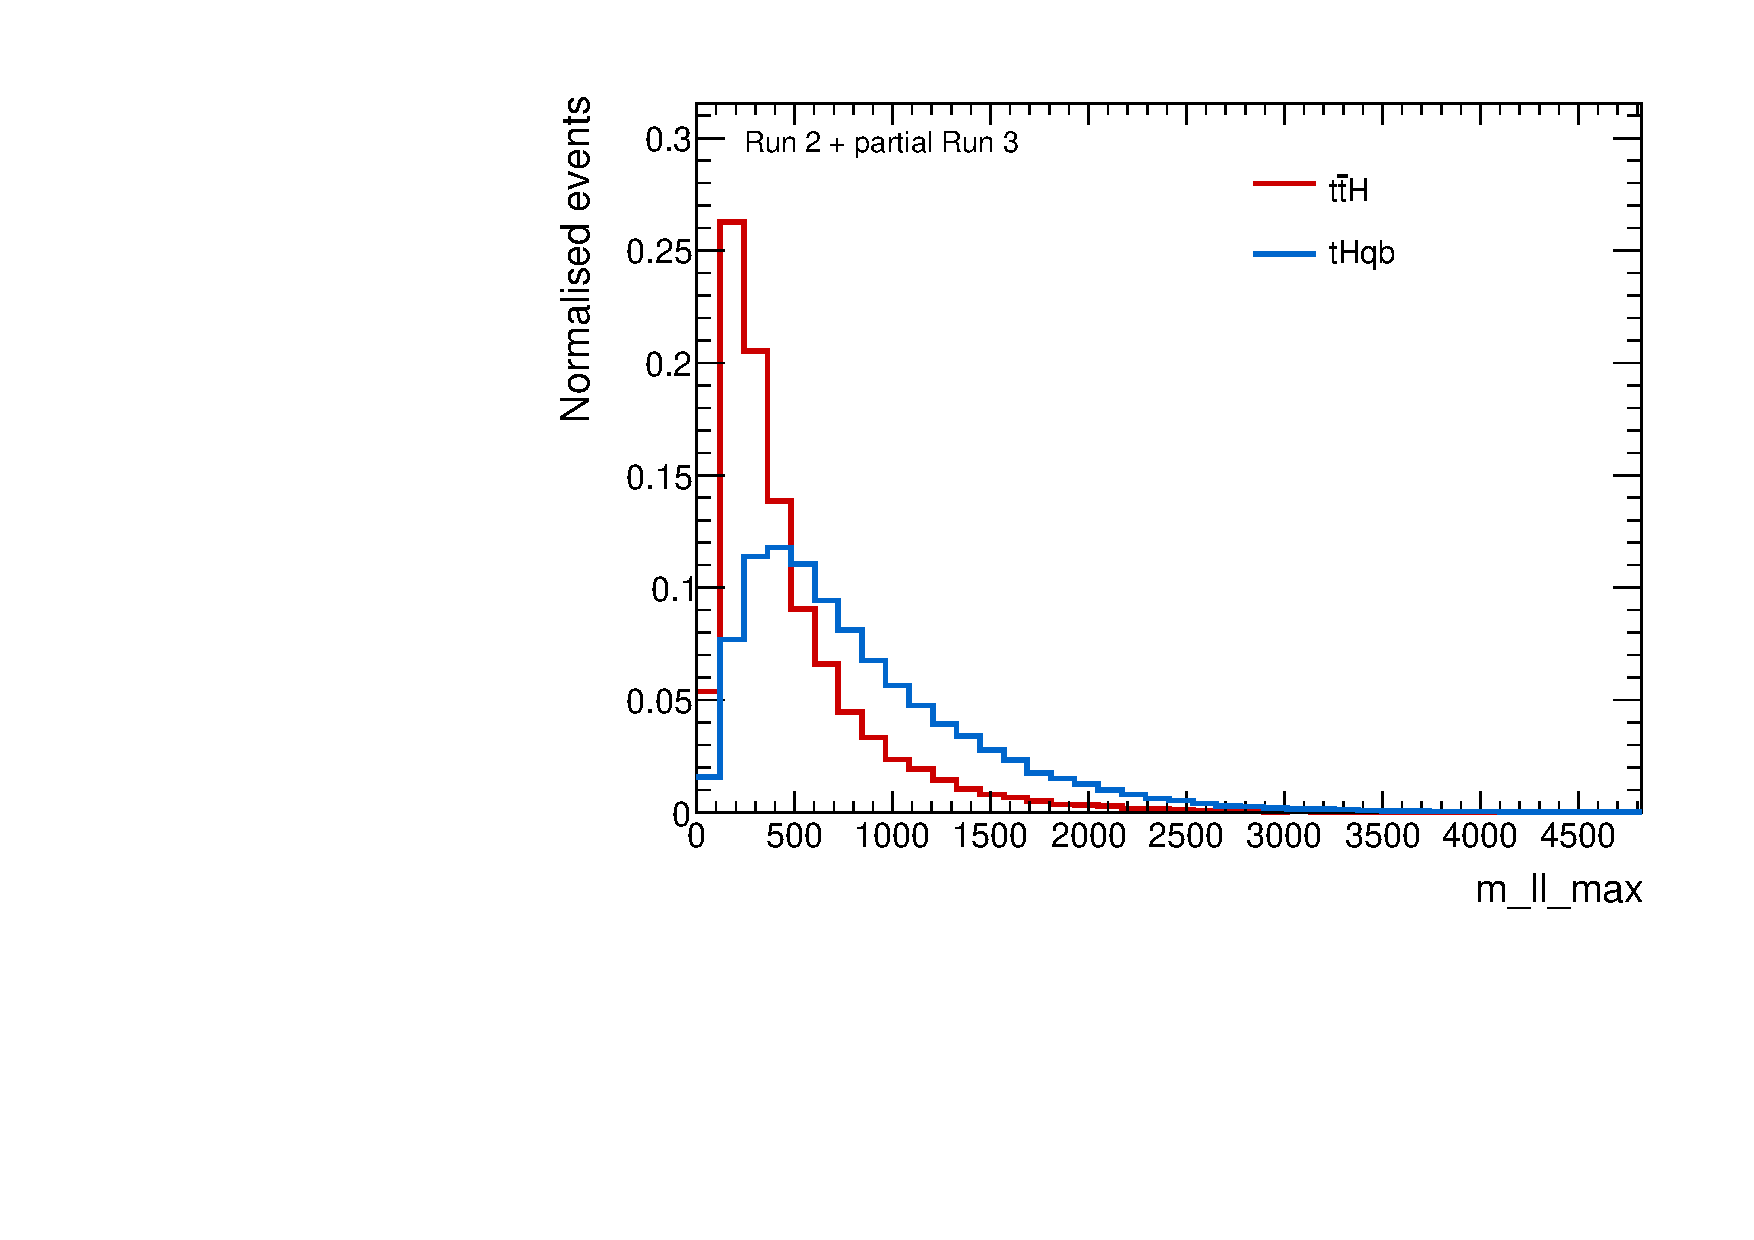
\includegraphics[width=\textwidth]{images/plots_tH_tHqb_for_thesis/m_ll_max_signals_ATLAS.pdf}
    \caption{Largest invariant mass of two light jets}
    \label{fig:m_ll_max}
  \end{subfigure}

  \caption{Distribuciones de algunas de las variables de entrada adicionales utilizadas en el entrenamiento del BDT, mostradas para eventos simulados de \thqb y \ttH después de los cortes de preselección.
  }
  \label{res:new_variables}
\end{figure}

Las regiones del análisis (SRs y CRs) se definen con una regla de “clase ganadora”: cada evento se asigna a la región cuyo \emph{score} es máximo entre los cuatro. Para reforzar la pureza en SRs, se mantiene la estrategia previa de dividir las SRs de \ttH\ y \thqb en \emph{window} ($100<m^{\text{MMC}}_{\tau\tau}<150$~GeV) y \emph{sidebands}. En este análisis, la \mmc deja de ser la variable de entrada del ajuste, y ahora se incluye como variable de entrada en el BDT, lo que reduce visiblemente las posibles colas de eventos de \ttbar en las SRs. 
Ahora el ajuste estadístico se construye sobre las distribuciones de los \emph{scores} en sus SRs y CRs correspondientes, con un binning optimizado que garantiza incertidumbre estadística relativa del fondo $<20\%$ en todos los bins y un mínimo de eventos ($\ge 3$ en SRs, $\ge 20$ en CRs). En las Figuras~\ref{res:fit_inputs_1}-\ref{res:fit_inputs_3} se muestran las distribuciones de entrada para el fit.

\begin{figure}[htbp]
  \centering
  % Run-2
  \begin{subfigure}[t]{0.45\textwidth}
    \centering
    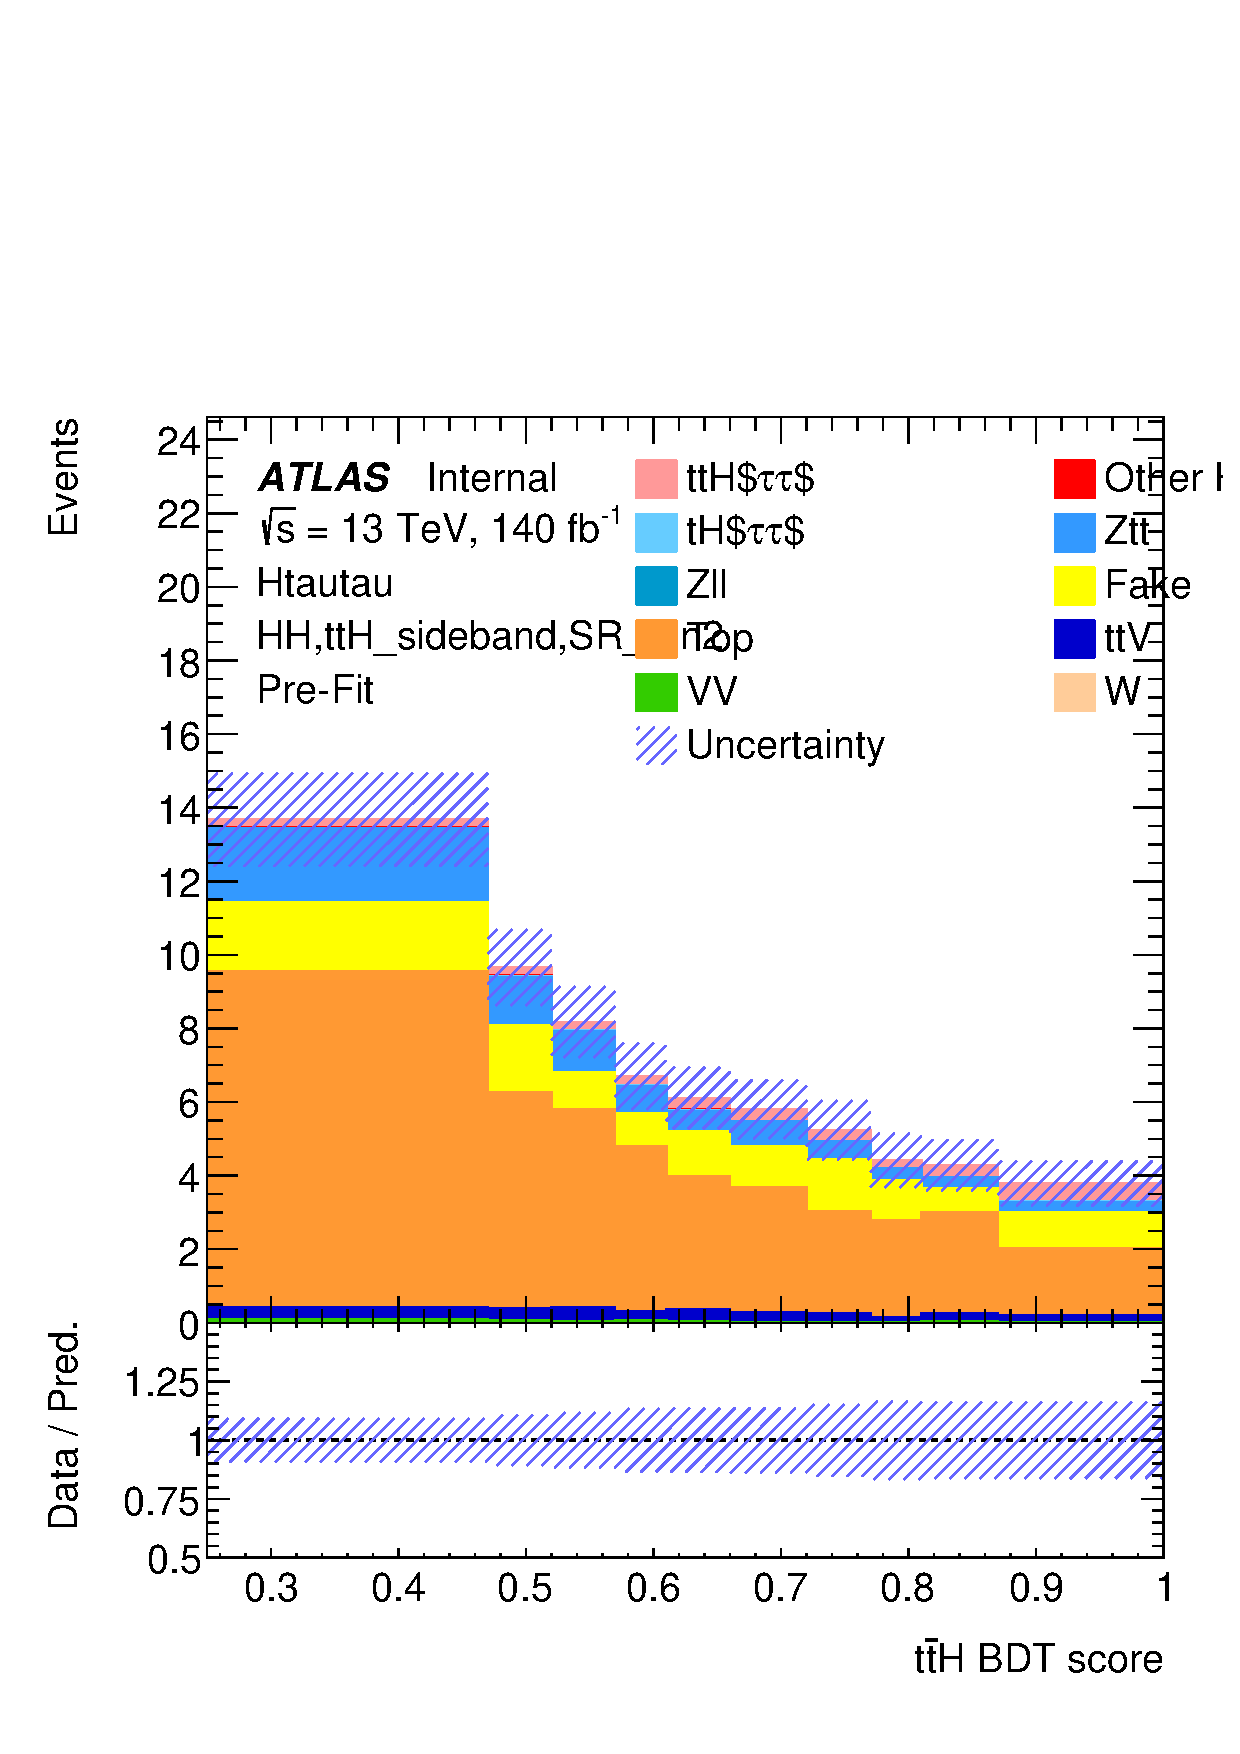
\includegraphics[width=\linewidth]{asimov_fit_th_tth/prefit/chan_hh_run2_cat_tth_tth_sideband__sr.pdf}
    \caption{Run-2, $t\bar{t}H$ sideband SR}
  \end{subfigure}
  \hfill
  \begin{subfigure}[t]{0.45\textwidth}
    \centering
    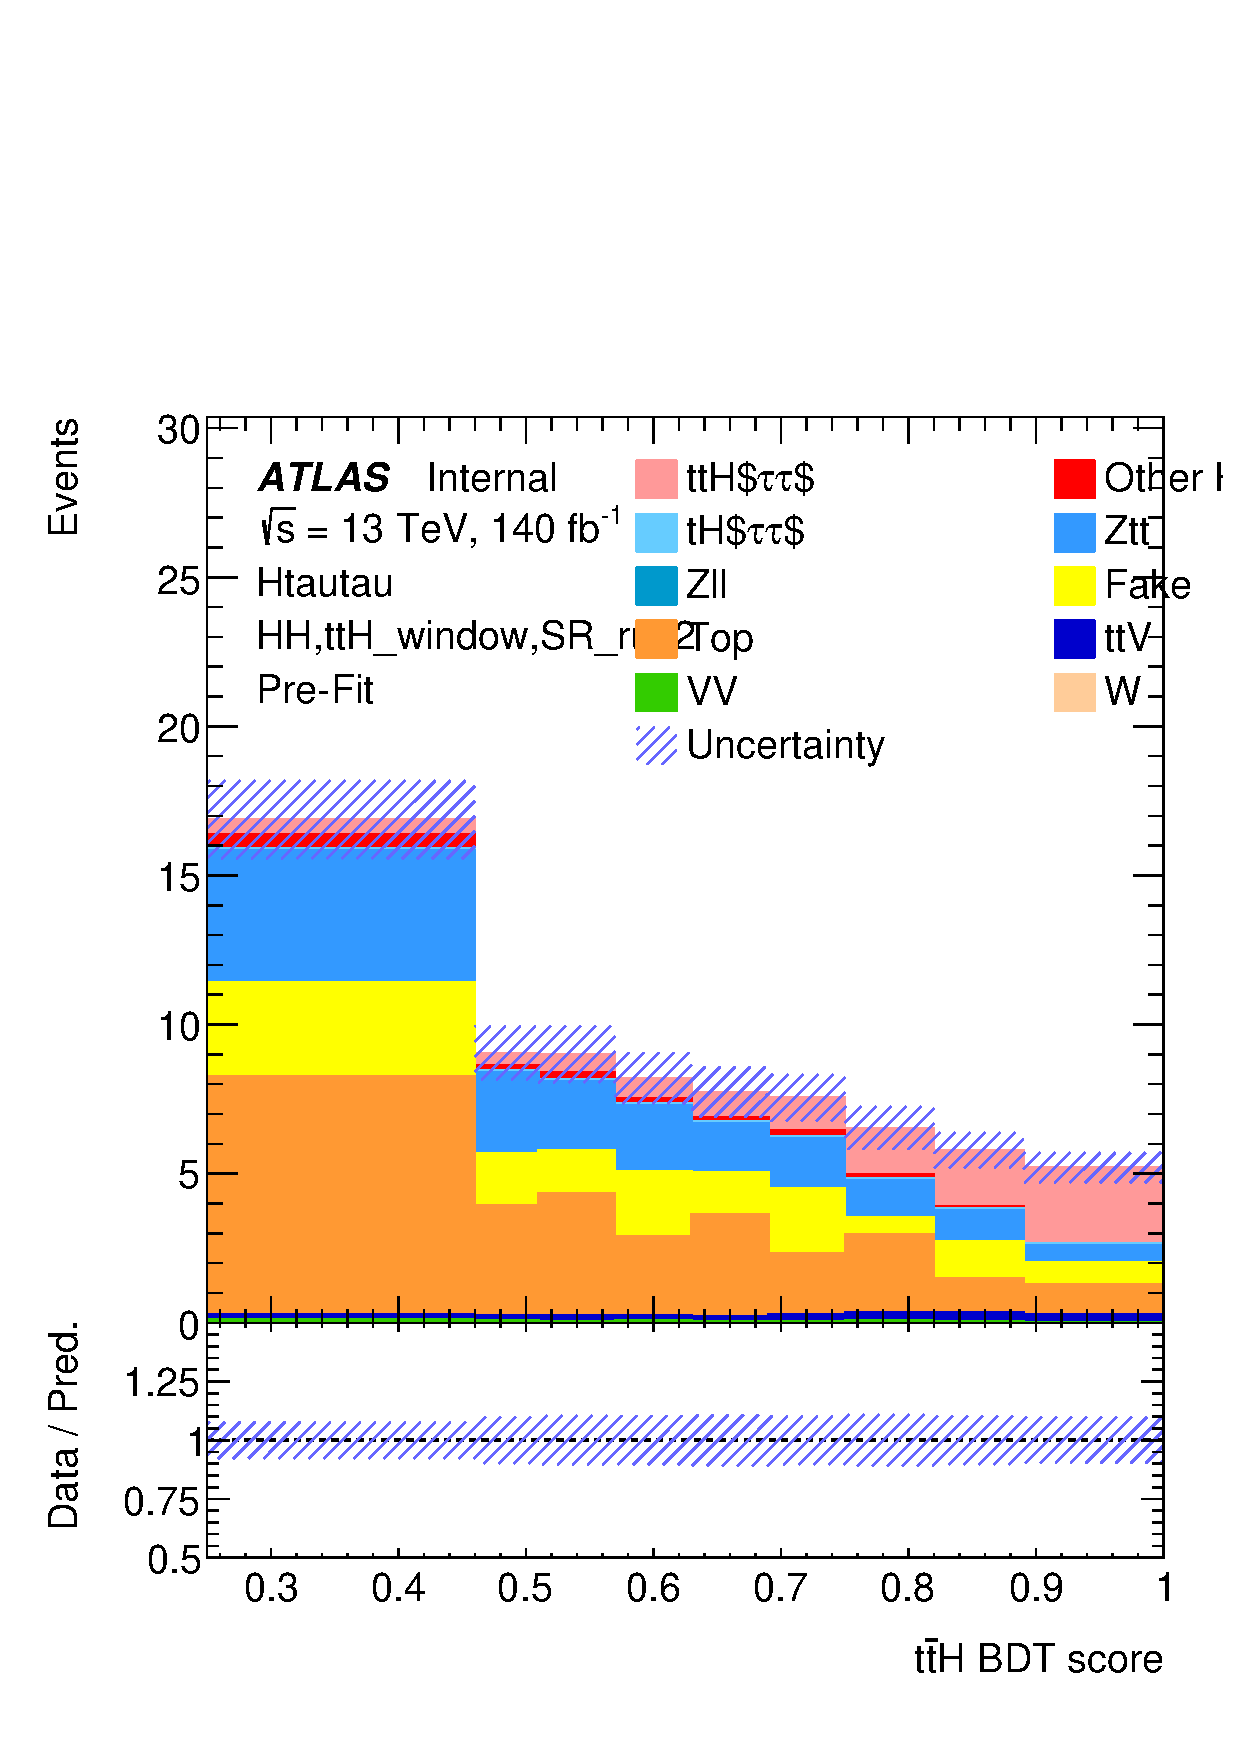
\includegraphics[width=\linewidth]{asimov_fit_th_tth/prefit/chan_hh_run2_cat_tth_tth_window__sr.pdf}
    \caption{Run-2, $t\bar{t}H$ window SR}
  \end{subfigure}

  % Run-3
  \vspace{0.4cm}
  \begin{subfigure}[t]{0.45\textwidth}
    \centering
    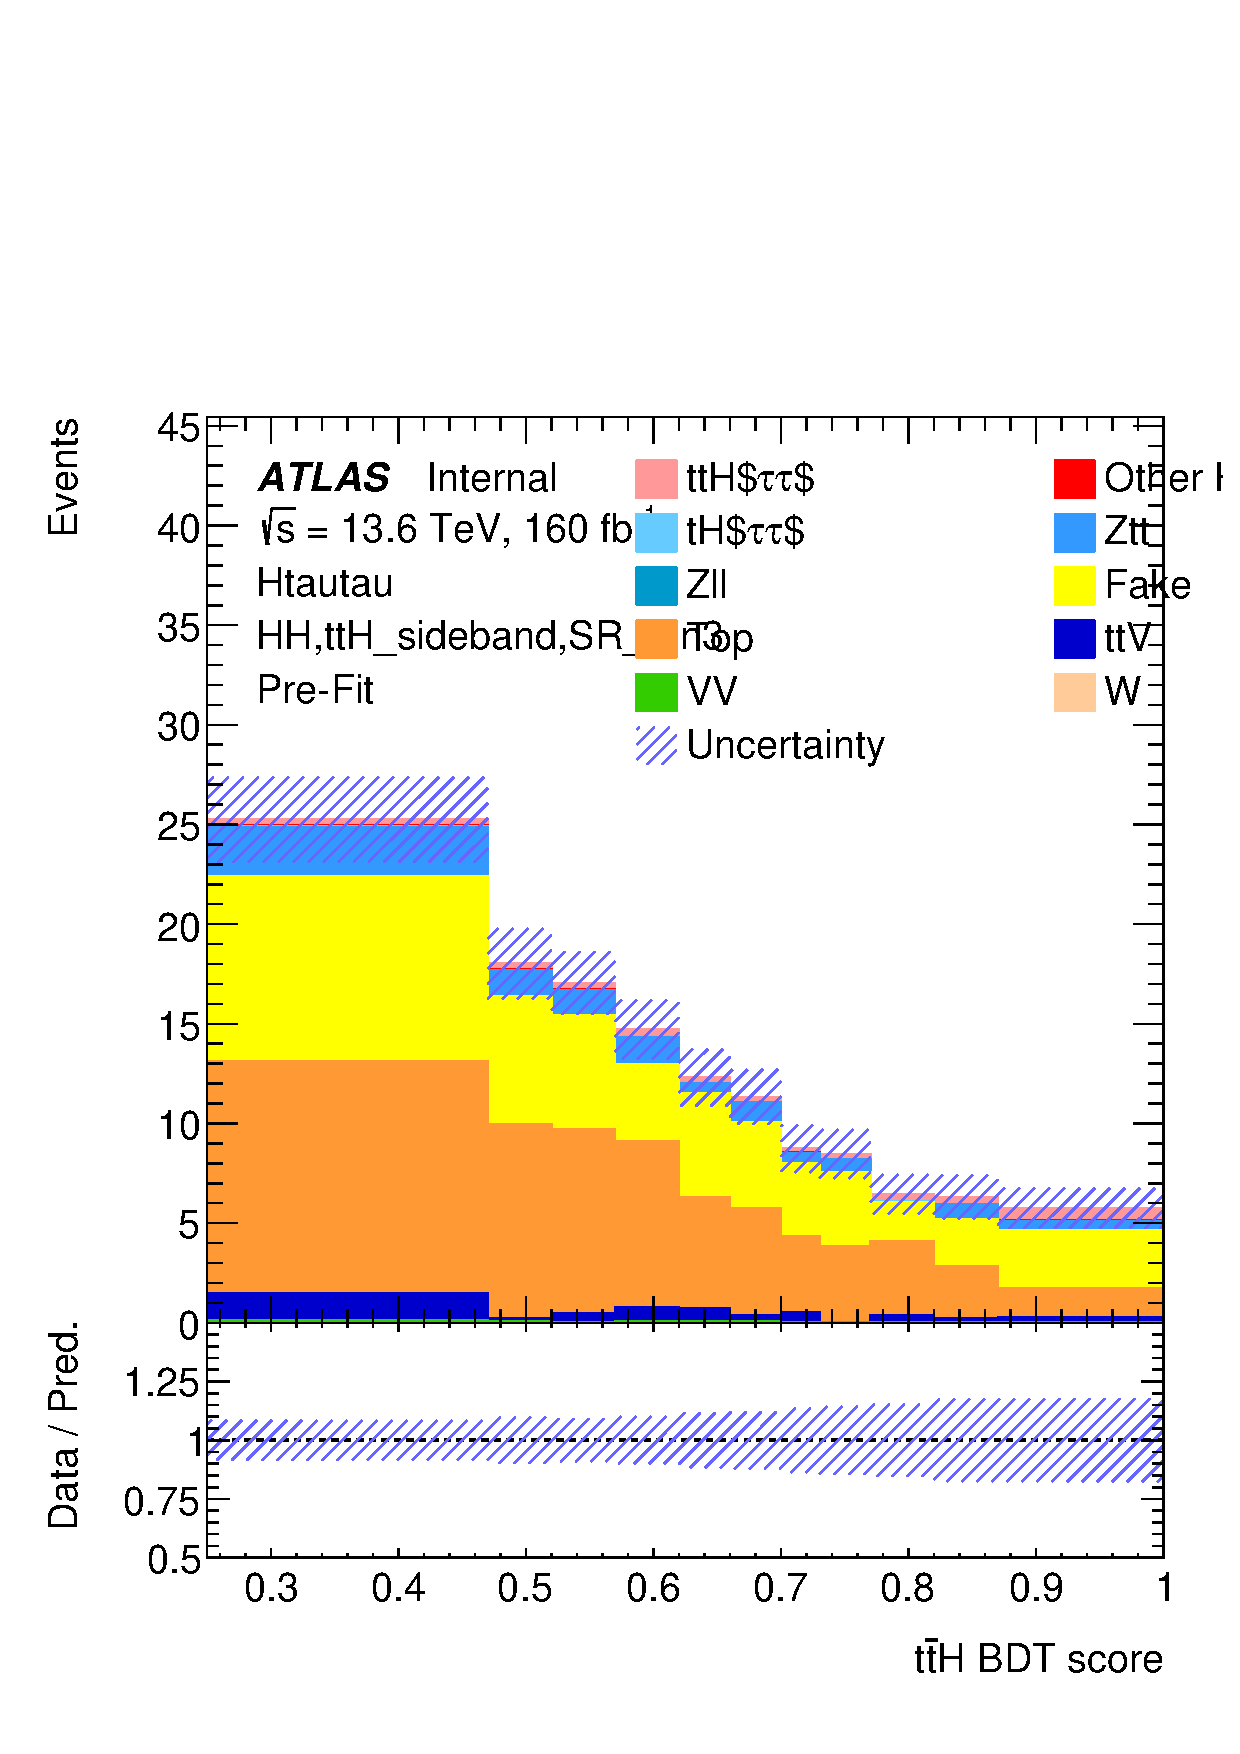
\includegraphics[width=\linewidth]{asimov_fit_th_tth/prefit/chan_hh_run3_cat_tth_tth_sideband__sr.pdf}
    \caption{Run-3, $t\bar{t}H$ sideband SR}
  \end{subfigure}
  \hfill
  \begin{subfigure}[t]{0.45\textwidth}
    \centering
    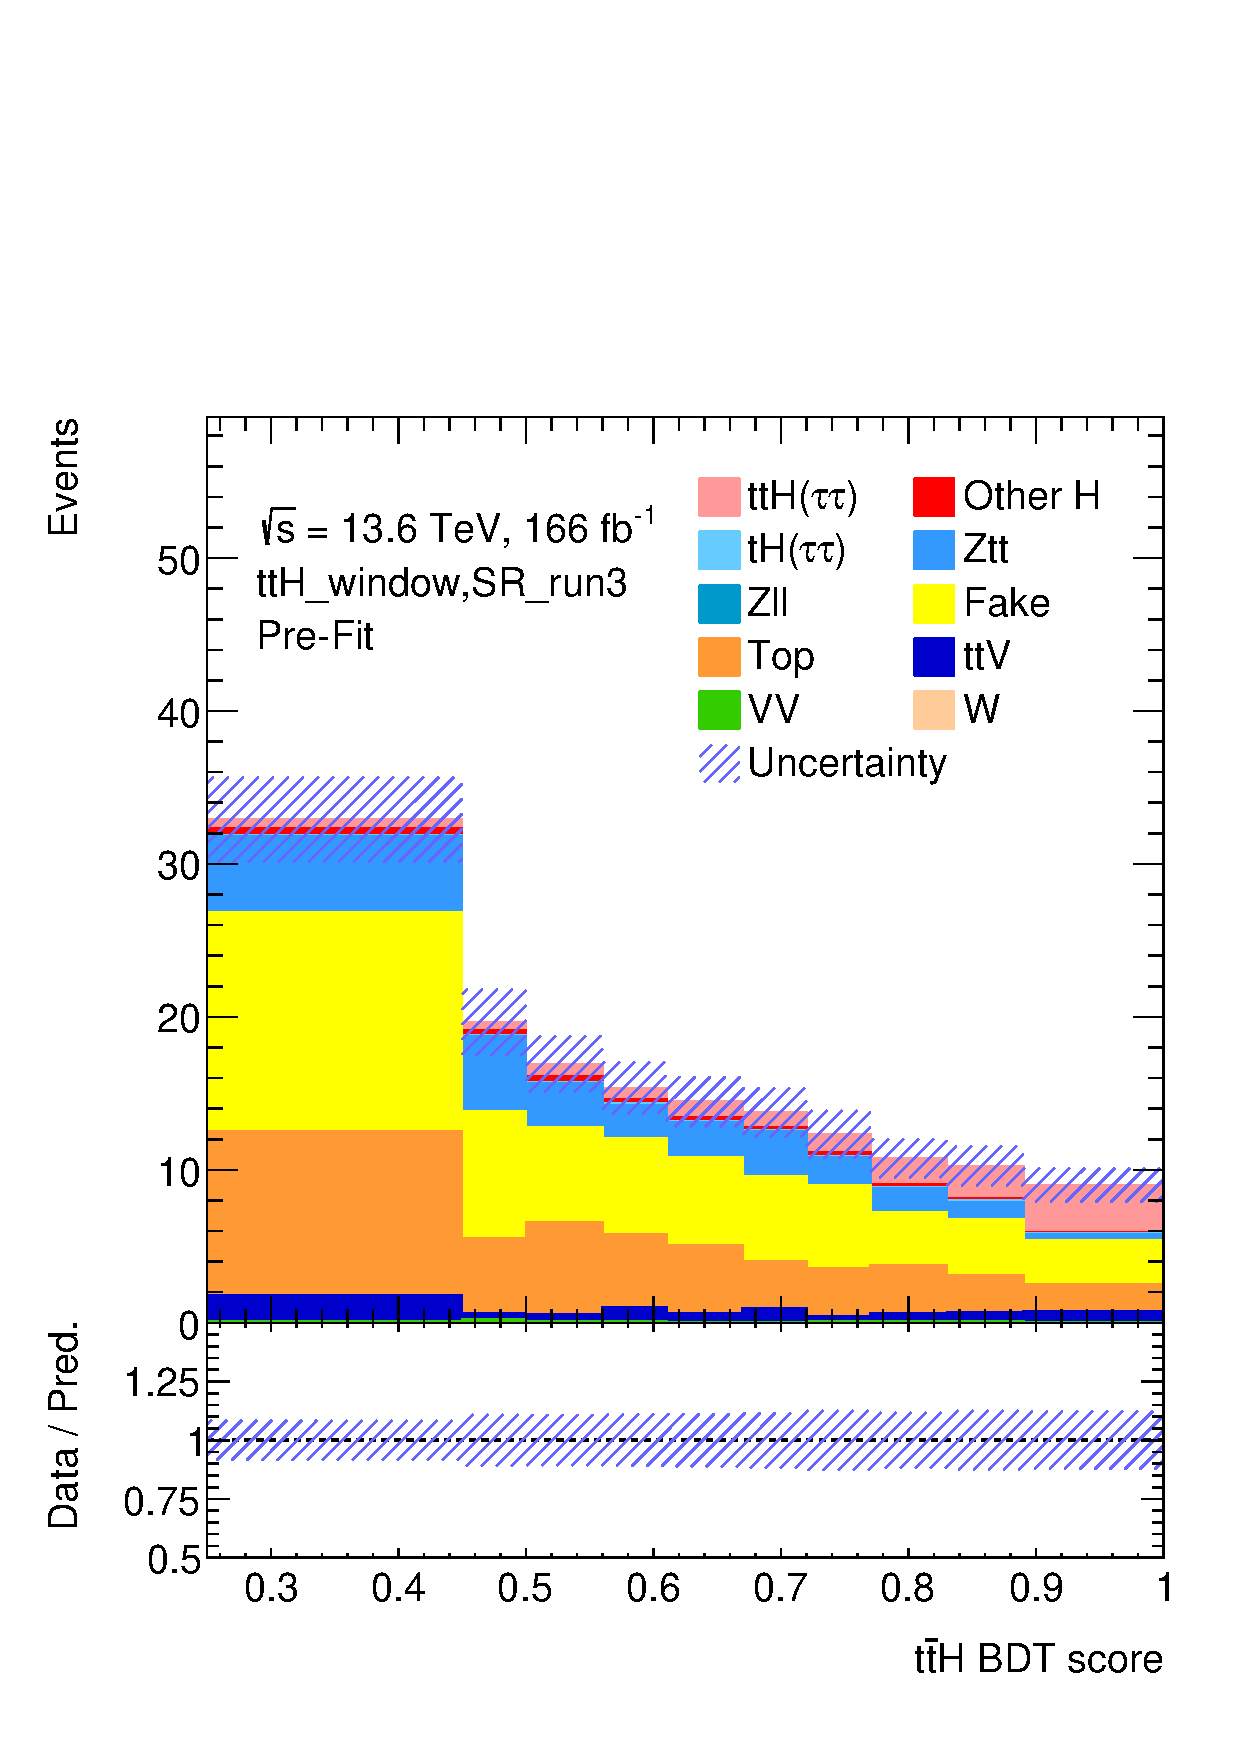
\includegraphics[width=\linewidth]{asimov_fit_th_tth/prefit/chan_hh_run3_cat_tth_tth_window__sr.pdf}
    \caption{Run-3, $t\bar{t}H$ window SR}
  \end{subfigure}

  \caption{SRs for $t\bar{t}H$ antes del fit, mostradas por separado para Run~2 yRun~3. No se aplican factores de escala \ztautau o \ttbar. Solo se consideran incertidumbres estadísticas.}
  \label{res:fit_inputs_1}
\end{figure}


\begin{figure}[htbp]
  \centering
  % Run-2
  \begin{subfigure}[t]{0.45\textwidth}
    \centering
    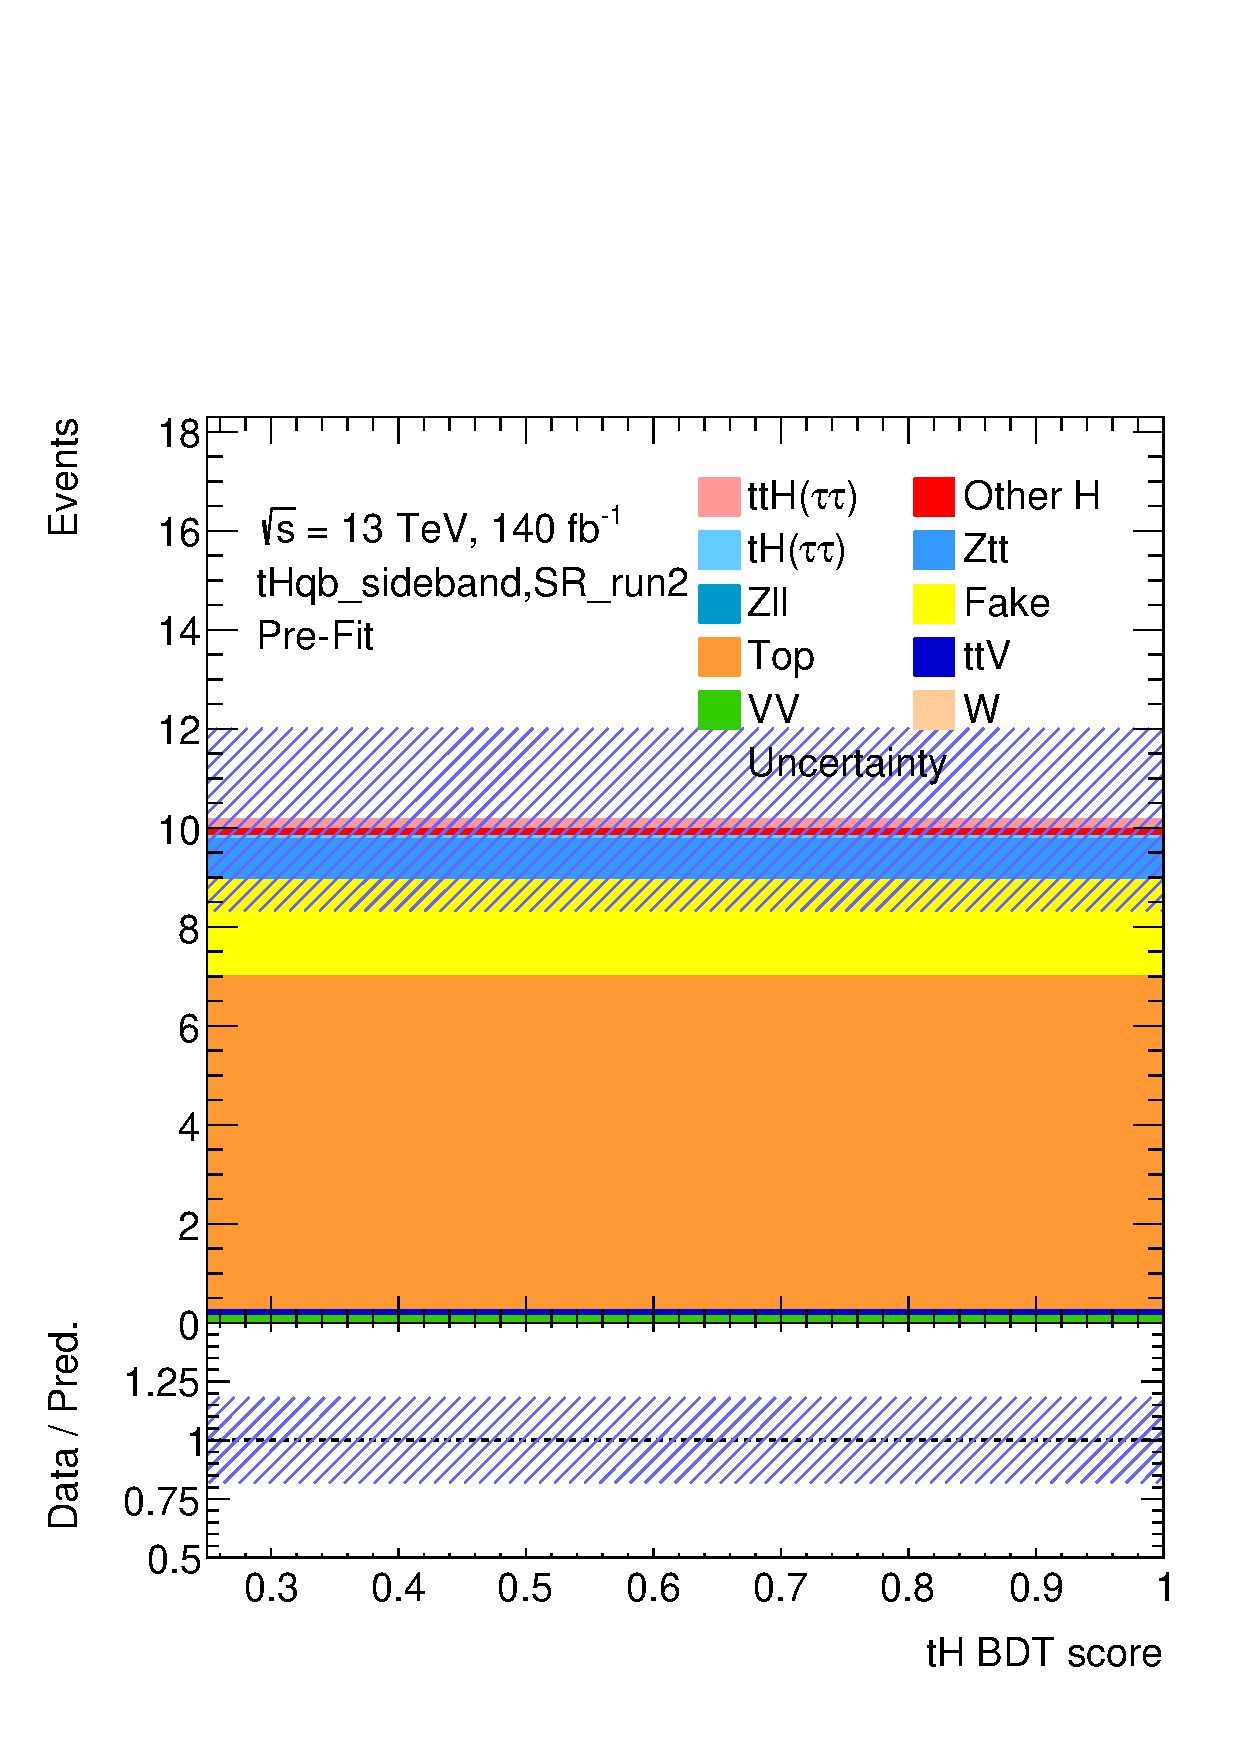
\includegraphics[width=\linewidth]{asimov_fit_th_tth/prefit/chan_hh_run2_cat_tth_th_sideband__sr.pdf}
    \caption{Run-2, $tHqb$ sideband SR}
  \end{subfigure}
  \hfill
  \begin{subfigure}[t]{0.45\textwidth}
    \centering
    \includegraphics[width=\linewidth]{asimov_fit_th_tth/prefit/chan_hh_run2_cat_tth_th_window__sr.pdf}
    \caption{Run-2, $tHqb$ window SR}
  \end{subfigure}

  % Run-3
  \vspace{0.4cm}
  \begin{subfigure}[t]{0.45\textwidth}
    \centering
    \includegraphics[width=\linewidth]{asimov_fit_th_tth/prefit/chan_hh_run3_cat_tth_th_sideband__sr.pdf}
    \caption{Run-3, $tHqb$ sideband SR}
  \end{subfigure}
  \hfill
  \begin{subfigure}[t]{0.45\textwidth}
    \centering
    \includegraphics[width=\linewidth]{asimov_fit_th_tth/prefit/chan_hh_run3_cat_tth_th_window__sr.pdf}
    \caption{Run-3, $tHqb$ window SR}
  \end{subfigure}

  \caption{SRs for \thqb antes del fit, mostradas por separado para Run~2 yRun~3. No se aplican factores de escala \ztautau o \ttbar. Solo se consideran incertidumbres estadísticas.}
  \label{res:fit_inputs_2}
\end{figure}

\begin{figure}[htbp]
  \centering
  % Run-2
  \begin{subfigure}[t]{0.45\textwidth}
    \centering
    \includegraphics[width=\linewidth]{asimov_fit_th_tth/prefit/chan_hh_run2_cat_tth_ttbar__cr.pdf}
    \caption{Run-2, $t\bar{t}$ CR}
  \end{subfigure}
  \hfill
  \begin{subfigure}[t]{0.45\textwidth}
    \centering
    \includegraphics[width=\linewidth]{asimov_fit_th_tth/prefit/chan_hh_run2_cat_tth_Ztt__cr.pdf}
    \caption{Run-2, $Z\to\tau\tau$ CR}
  \end{subfigure}

  % Run-3
  \vspace{0.4cm}
  \begin{subfigure}[t]{0.45\textwidth}
    \centering
    \includegraphics[width=\linewidth]{asimov_fit_th_tth/prefit/chan_hh_run3_cat_tth_ttbar__cr.pdf}
    \caption{Run-3, $t\bar{t}$ CR}
  \end{subfigure}
  \hfill
  \begin{subfigure}[t]{0.45\textwidth}
    \centering
    \includegraphics[width=\linewidth]{asimov_fit_th_tth/prefit/chan_hh_run3_cat_tth_Ztt__cr.pdf}
    \caption{Run-3, $Z\to\tau\tau$ CR}
  \end{subfigure}

  \caption{CRs for \ttbar y \ztautau antes del fit, mostradas por separado para Run~2 yRun~3. No se aplican factores de escala \ztautau o \ttbar. Solo se consideran incertidumbres estadísticas.}
  \label{res:fit_inputs_3}
\end{figure}

La interpretación estadística sigue la misma arquitectura que el análisis anterior, pero en un marco independiente, sin incluir el análisis de estos modos de producción en la combinación global de \htautau. 
Se consideran dos parámetros de interés globales, $\mu_{\ttH}$ y $\mu_{\thqb}$, y factores de normalización libres para $Z\to\tau\tau$ y $\ttbar$, separados para Run~2 y Run~3. En el estudio aquí presentado solo se incluyen incertidumbres estadísticas para estudiar la sensibilidad esperada.

Con el ajuste Asimov, realizado sobre una muestra de pseudo-datos centrados entorno a los valores esperados para los distintos parámetros de ajuste, la precisión esperada en los NFs de $Z\to\tau\tau$ y $\ttbar$ se sitúa en el 6–8\%, mejorando un 60–70\% lo visto en el capítulo anterior, y la sensibilidad prevista para \ttH alcanza $\Delta\mu_{\ttH}=^{+0.54}_{-0.51}$, mejor que la de la medida inclusiva previa en \htautau. Para \thqb la precisión esperada es sustancialmente más débil, $\Delta\mu_{\thqb}=^{+4.72}_{-4.20}$, puesto que es un proceso para el cual sufríamos de baja estadística; además, los dos POIs aparecen fuertemente anticorrelacionados (–39\%), en línea con la tasa de confusión que se obtenía de los discriminantes entrenados en el BDT.

Para validar el control de los fondos en datos y justificar la aplicación de los factores de escala en distribuciones de Run~3, se repite el ajuste incorporando datos en las CRs y manteniendo \textit{blinded} las SRs. Las distribuciones tras el ajuste reproducen con buena calidad los datos, y los NFs resultantes se muestran en la Tabla~\ref{res:nfs_data},
\begin{table}[h]
  \small
  \centering
  \caption{NFs para \ztautau and \ttbar en Run~3 y Run~2 usando datos en las CRs.}
  \renewcommand{\arraystretch}{1.25}
  \setlength{\tabcolsep}{10pt}
  \begin{tabular}{lcc}
    \toprule
    \textbf{Process} & \textbf{Run-3 $NF$} & \textbf{Run-2 $NF$} \\
    \midrule
    \ztautau              & $1.47^{+0.08}_{-0.08}$ & $1.12^{+0.07}_{-0.07}$ \\
    \ttbar       & $1.22^{+0.08}_{-0.08}$ & $1.10^{+0.09}_{-0.08}$ \\
    \bottomrule
  \end{tabular}
  \label{res:nfs_data}
\end{table}
siendo consistentes con las estimaciones ilustrativas 1.4 (\ztautau) y 1.2 (\ttbar) que se habían empleado, y compatibles con la ronda anterior en Run~2 dentro de incertidumbres.

En conjunto, la inclusión explícita de \thqb en la estrategia multivariante y la categorización con el uso de discriminantes habilita un análisis coherente y potencialmente sensible a la estructura de $CP$ en el vértice $Ht\bar t$, manteniendo un control sólido de los fondos dominantes con datos en CRs. La mejora prevista para \ttH respecto a la ronda anterior y la sensibilidad alcanzable para \thqb (en el contexto de este canal y esta estadística) son consistentes con las expectativas del modelo y los resultados recientes en otros modos y canales de ATLAS y CMS~\cite{Sirunyan_2021, 2025, ATLAS:2025irr, thgammagamma} sin que se aprecien tensiones al incorporar los datos parciales de Run~3.
